% TODO: Formulierung als OCP anstelle MPC in anschließenden Kapiteln erwähnen
% Story:
% Trajektorienplanung -> OSP
% Allg. Formulierung OSP
% Fahrzeugspez. Formulierung OSP
% Ausblick auf Lösungsmethodik:
% - Modifikation der Problemstellung bei DP und DM
% OS -> Rückkopplung -> Stabilitätsbetrachtungen
% Stabilität v. Lyapunov -> Lyapunovfunktion
% Stabilität von MPC, unendlicher, quasiunendlicher Opt.-Horizont
% Robustheitssteigerung druch unterl. Regelung
%  - ...
%  - Praxiserprobte unterlagerte Regler
% Beispiel Gespann
% Ausblick auf nachfolgende Kapitel zur OSP
\chapter{Stabilität und Robustheit optimaler Fahrmanöver}\label{chap:stabilisierung}
\zitat{If everything is under control \\
you are just not driving fast enough.}{Sir Stirling Moss}


Aufgrund der theoretisch unendlich vielen Möglichkeiten bei der Planung einer Fahrtrajektorie muss eine Bewertung in einem bestimmten Sinne vorgenommen werden, um die \emph{beste} Trajektorie wählen zu können. Diese Herangehensweise wird als Optimierung bezeichnet. Wie hierzu in \cite{foellingeroptimal} angemerkt wurde, wird jedoch im gängigen Sprachgebrauch der Begriff \emph{optimal} vergleichsweise sorglos gebraucht, und der Eindruck erweckt, dass schon von Optimieren die Rede ist, wenn lediglich die Bearbeitung einer Aufgabe gezielt angegangen wird. Die mathematische Formulierung eines Optimierungsproblems erfordert allerdings stets eine genaue Definition der Optimierungsvariablen\index{Optimierungsvariable} und des Gütekriteriums\index{Gütekriterium}. Motiviert durch das vorangegangene Kapitel widmet sich das vorliegende deshalb der Formulierung des Optimalsteuerungsproblems\index{Optimalsteuerung} der automatisierten Fahraufgabe, welches sich aus der Fahrzeugumfeldinformation, der zeitlichen Prädiktion der dynamischen Hindernisse, der Eigenfahrzustandsschätzung und dem eigentlichen Optimierungsziel ableitet.

Des Weiteren spielt die Optimalität eine entscheidende Rolle bei den Untersuchungen zur Stabilität des modellprädiktiven Regelkreises, der durch die im Optimalsteuergesetz permanent rückgekoppelten Systemzustände entsteht. %, s.\ Abschn.\,\ref{sec:def_modellpraediktive_Regelung}. %Aufgrund der beschränkten Rechenleistung ist immer nur die Betrachtung eines endlichen Optimierungshorizonts möglich
Die in diesem Kapitel vorgenommenen Betrachtungen geben dabei, vor dem Hintergrund eines aus technischen Gründen zeitlich beschränkten Optimierungshorizonts, wichtige Hinweise darauf, wie das Optimalsteuerungsproblem zu formulieren ist, um nicht nur das Gesamtverhalten einer Fahrerassistenzfunktion zu verbessern, sondern auch Stabilitätsgarantien auszusprechen.  


Darüber hinaus wird der Einsatz unterlagerter Regler im modellprädiktiven Regelkreis systematisiert, der \ua auf eine Verbesserung der Robustheitseigenschaften des Gesamtsystems bzgl.\ Störungen und Modellfehlern abzielt. In der Praxis zeigt sich nämlich, dass ein tieferes Verständnis über die keinesfalls trivialen Wechselwirkungen innerhalb des modellprädiktiven kaskadierten Regelkreises essentiell für die Auslegung der unterlagerten Fahrzeugregler ist.

Schließlich wird der Entwurf und die prototypische Implementierung eines neuartigen Assistenzsystems der Stabilisierungsebene vorgestellt, welches das Ziel verfolgt, den Fahrzeugführer beim Zurücksetzen und Rangieren mit Anhänger bestmöglich zu unterstützen. Ganz im Sinne des zuvor diskutierten kaskadierten Regelkreises stellt hierbei der Fahrer den Führungsregler dar, verbunden durch eine geeignete Mensch-Maschine-Schnittstelle mit dem unterlagerten Regler, der automatisch die Stabilisierung des Anhängers durch aktive Lenkeingriffe vornimmt. Der entsprechende Abschnitt~\ref{sec:anhaenger} wurde bereits in großen Teilen in den eigenen Arbeiten \citeltex{werling2014anhaenger, Werling2014trailer} veröffentlicht und übernommene Texte sind nicht gesondert gekennzeichnet.

%Die entsprechenden Kapitelinhalte wurden bereits im Rahmen von \citeltex{werling2014anhaenger, Werling2014trailer} veröffentlicht. anh

% Trotz einleitenden Zitats: Ernst zu nehmendes Thema, da Fahrzeug 2T schwer und schnell.
% In der Robotik häufig vernachlässigtes Problem. Die Regelungstechnik ist sich der Problematik ums so mehr bewusst.
		
	% Modelle und Theorien zur Beschreibung der Fahraufgabe und des Fahrerverhaltens: Carsten, O.: From Driver Models to Modelling the Driver: What Do We Really Need to Know About the Driver? In: (Hrsg.), Cacciabue (Hrsg.): Modelling Driver Behaviour in Automotive Environments. Springer-Verlag Limited, 2007
%Bedeutung von Heuristiken, 
	% Neuplanung kann sehr selten beim Einparken erfolgen, hier deshalb positionsstabilisierung
	% Drei Schritte zur Robustheit: optimale Steuerung, unterlagerte Regelung, Neuplanung (optimale Regelung) robust gegen Störungen Modell Fehler und sich ändernde Umgebungen
	% Neuplanung wichtig für: 1) Berücksichtigung neuer Information über Umfeld 2) Information über Systemzustand (Stabilität und Störungsrobustheit!)

\section{Manöverplanung als Optimalsteuerungsproblem} \label{sec:unendlichdim_opt}
Im Unterschied zur \emph{statischen} Optimierung\index{statische Optimierung}, welche sich der Optimierung von \emph{Parametern} widmet, s.\ später Abschn.\,\ref{sec:statischeOptimierung}, stellen bei der \emph{dynamischen} Optimierung\index{dynamische Optimierung} \emph{Funktionen} $\bs{x}(t)$ einer unabhängigen Variablen $t$ (\zB die Zeit) die Entscheidungsvariablen dar \cite{foellingeroptimal, bertsekas2007, papageorgiou2012optimierung}. Es wird in dem Zusammenhang auch von \emph{unendlich-dimensionaler} Optimierung gesprochen. Zur Bewertung einer Funktion $\bs{x}(t)$ bedarf es dann einer Abbildung des \emph{Funktionen}raumes $\mathbb R^n$ in die Menge $\mathbb R$ der reellen Zahlen, welche auch als Güte\emph{funktional}\index{Gütekriterium} ("`Funktion von Funktionen"' \cite{papageorgiou2012optimierung}) bezeichnet wird. \\
Aufgrund des Fokus auf die Fahrzeuganwendung wird an dieser Stelle ein in der Regelungstechnik und Robotik weit verbreiteter Sonderfall der dynamischen Optimierung betrachtet, bei dem die optimale Eingangstrajektorie $\bs{u^\ast}(t)$ für ein dynamisches System gesucht wird, das sog.\ \emph{Optimalsteuerungsproblem}\index{Optimalsteuerung}.
%Dies trifft insbesondere auf die Optimierung von Fahrtrajektorien zu. 


\subsection{Mathematische Formulierung}
%\subsection{Problemformulierung dynamische Optimierung} 
\label{sec:direkte_opt_dynamisch}
Eine recht allgemeine und daher in der Literatur häufig anzutreffende Struktur des Optimalsteuerungsproblems lautet \cite{graichen2014SkriptOpt}:

\quad Minimiere das Kostenfunktional\footnote{Während der Begriff \emph{Gütefunktional} bei der Optimierung eine Maximierung impliziert, zielt der Begriff \emph{Kostenfunktional} auf eine Minimierung ab. In der Literatur werden die Begriffe synonym verwendet \cite{papageorgiou2012optimierung}, da eine gegenseitige Überführung lediglich ein Vorzeichenwechsel der Bewertungsfunktionale bedeutet.} %Entsprechendes gilt später für die Funktionale der dynamischen Optimierung.}
%
\begin{subequations} \label{equ:optimalsteuerungsproblem}
\begin{align} \label{equ:opt_funktional}
	J(\bs{u}(t)) = \int_{t_0}^{t_f} l(\bs{x}(t),\bs{u}(t),t)\,{\rm d} t \,\,+\,\, V(\bs{x}(t_f),t_f)
\end{align}
\quad unter Berücksichtigung der Systemdynamik 
\begin{align} 	\label{equ:opt_systemdynamik}
	\dot{\bs{x}}(t) = \bs{f}(\bs{x}(t),\bs{u}(t),t), \quad &\bs{x}(t_0) = \bs{x}_0 
\end{align} 
\quad sowie der Gleichungs- und Ungleichungsbeschränkungen 
\begin{align} 	
	\bs{g}(\bs{x}(t_f),t_f) &= \bs{0}  \label{equ:zm} \\ 	
	\bs{h}(\bs{x}(t),\bs{u}(t),t) & \leq \bs{0},  \quad \forall t \in[t_0, t_f] 	\label{equ:opt_ungleichungen} \;. 
\end{align} 
\end{subequations}
\begin{figure}[ht]
\psfrag{1}[cr][cr][1.0]{$x_1$}
\psfrag{2}[br][br][1.0]{$x_2$}
\psfrag{x}[tc][tc][1.0]{$\bs{x}^\ast(t)$}
\psfrag{0}[cr][cr][1.0]{$\bs{x}_0$}
\psfrag{e}[tl][tl][1.0]{$t_f$}
\psfrag{o}[tl][tl][1.0]{$t_0$}
\psfrag{t}[bc][bc][1.0]{$t$}
\psfrag{g}[bc][bc][1.0]{$\bs{g}=\bs 0$}
\psfrag{h}[tc][tc][1.0]{$h>0$}
	\centering
  	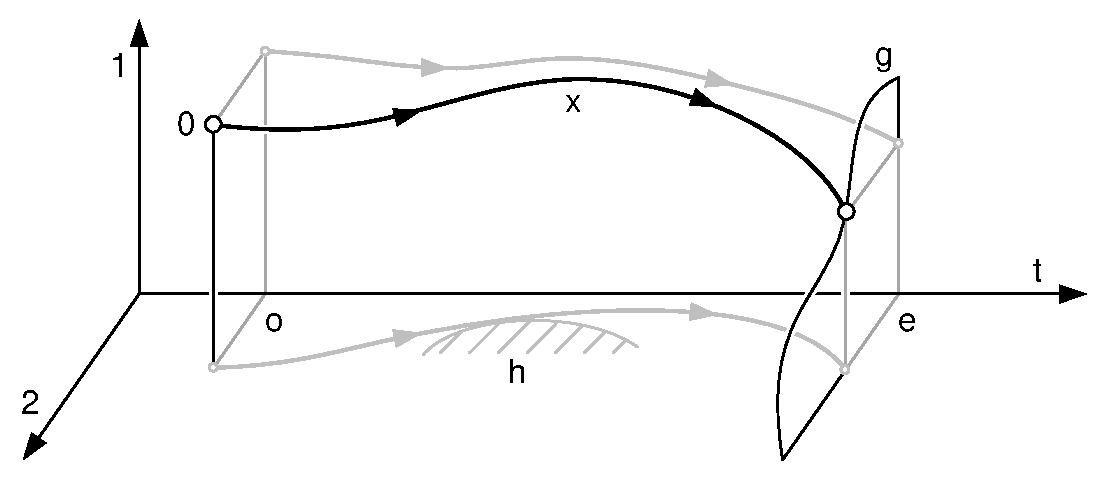
\includegraphics[width=1.\textwidth,clip, trim = 0cm 0cm 0cm 0cm]{2_Darstellung_dynamische_Optimierung_endvorgabe.eps}
  	\caption[Veranschaulichung der Lösung des Optimalsteuerungsproblems]{Veranschaulichung der Lösung $\bs{x}^\ast (t)\in \mathbb{R}^2$ eines Optimalsteuerungsproblems mit Endbedingung $\bs{g}=\bs 0$ und Ungleichungsbeschränkung $h\leq 0$ für $x_2$ sowie fester Endzeit $t_f$}
    \label{fig:dynamische_Optimierung_endvorgabe}
\end{figure}

Mit anderen Worten: Gesucht ist für ein (i.Allg.\ nichtlineares und zeitvariantes) System mit Zustand $\bs{x} \in \mathbb R^n$ und Eingang $\bs{u} \in \mathbb R^m$ auf dem Intervall $t\in[t_0, t_f]$ die Steuertrajektorie\index{Steuertrajektorie} $\bs{u}^\ast(t)$, die unter Minimierung des Kostenfunktionals\index{Kostenfunktional} $J$ das System vom Anfangszustand $\bs{x}_0$ in den Endzustand $\bs{x}(t_f)$ zur Endzeit $t_f$ steuert, sodass die Beschränkungen $\bs{h} \leq \bs{0}$ und Endbedingungen $\bs{g}= \bs{0}$ erfüllt sind, s.\ \abb{fig:dynamische_Optimierung_endvorgabe}. In der hier gewählten \emph{Bolza-Form} \cite{papageorgiou2012optimierung} setzt sich das Kostenfunktional \eqref{equ:opt_funktional} aus den Integralkosten $l$ und den Endkosten $V$ zusammen.\\
Die Endzeit $t_f$ ist entweder vorgegeben oder frei. Trifft letzteres zu, so ist $t_f$ Teil des Optimierungsproblems. Entfällt die Endbedingung $\bs{g}=\bs 0$, so wird von einem \emph{freien Endzustand} gesprochen. 
%Zur Veranschaulichung des Optimierungsproblems ist in \abb{fig:dynamische_Optimierung_endvorgabe} die optimale Trajektorie $\bs{x}^\ast(t)$ für eine feste Endzeit $t_f$ dargestellt. 
%In Bezug auf die f verschiedenen Auslegungsmöglichkeiten der Bestandteile des Optimalsteuerungsproblems im Hinblick auf das Trajektorien-Optimierungsproblem auf Fahrzeugführungsebene beleuchtet.

Zurückkehrend zu den Assistenzfunktionen der Führungsebene können die aufgeführten Bestandteile des Optimalsteuerungsproblems folgendermaßen ausgelegt werden:  Vereinfacht gesprochen\footnote{unter Vernachlässigung von Rückwirkungen der Bewegung des Eigenfahrzeugs auf die der anderen Verkehrsteilnehmer} findet sich die Fahrzeugdynamik und die daraus resultierende Bewegungskinematik im Systemmodell \eqref{equ:opt_systemdynamik} wieder. Unerwünschte Fahrzeugbewegungen, etwa das Abweichen von der Straßenmitte, gefährliche Fahrzustände, wie große Schwimmwinkel, und unkomfortable, hektische Lenkbewegungen sind im Kostenfunktional \eqref{equ:opt_funktional} zu bestrafen. Die Prädiktion der Fahrzeugumgebung wiederum fließt in die (aufgrund des dynamischen Fahrzeugumfelds \iA zeitvarianten) Ungleichungsbeschränkungen \eqref{equ:opt_ungleichungen} 
ein. Wie schon das Beispiel in Abb.\,\ref{fig:dynamische_Optimierung_endvorgabe} zeigt, kann darin die Kollisionsfreiheit inmitten von Hindernissen sichergestellt werden. Die Endbedingungen \eqref{equ:zm} können schließlich dazu genutzt werden, einen festen Zielzustand etwa auf einem Parkplatz vorzugeben. Darüber hinaus spielt die Wahl der Endkosten $V$ und der Ungleichungsbeschränkungen $\bs h$ eine entscheidende Rolle bei den Stabilitätsbetrachtungen in Abschn.\,\ref{sec:stab_mpc}.

\subsection{Modellprädiktiver Regelkreis\index{Modellprädiktiver Regelkreis}}
%[Unterbringen] Zur Erhöhung der Robustheit des Gesamtsystems gegen Störungen und Parameterschwankungen (Fahrbahnunebenheiten, nasse Fahrbahn), % und Ungenauigkeiten bei der Umsetzung der Trajektorie aufgrund von Parameterschwankungen und Modellvereinfachungen, 
%aber auch zur Berücksichtigung der jeweils aktuell verfügbaren Umfeldinformation empfiehlt sich eine permanente Neuplanung der Ausweichtrajektorie. Hierbei wird, im Unterschied zu einer initialen Einmalplanung, an der bis zum Manöverende festgehalten wird % (s.\ \zB 
%%\cite{keller2011active,% TITS Daimler, Polynome 7. Ordnung
%%isermann2008anticollision}, % sigmoiden
%%), 
%in jedem Zeitschritt der aktuelle Systemzustand in der Planung berücksichtigt, sodass aufgrund dieser Rückführung ein Regelkreis entsteht. \\
Erst durch eine permanente Berücksichtigung der aktuellen Umfeldinformationen ist eine optimale Navigation zwischen dynamischen Hindernissen möglich\footnote{Für singuläre Eingriffe wie dem Notausweichen existieren jedoch auch Forschungsansätze \cite{isermann2008anticollision, Bender2007, keller2011active}, die initial eine Trajektorie planen und an ihr bis zum Manöverende festhalten.}. Schließlich ist die Vorhersage der zukünftigen Bewegung anderer Verkehrsteilnehmer mit großen Unsicherheiten verbunden. Wie eingangs erwähnt, ermöglicht eine zyklische Optimierung aber auch die Reaktion auf unvorhergesehene Störungen bzw. Modellunsicherheiten. \\
Entsprechend der verbalen Beschreibung in Abschn.\,\ref{sec:def_modellpraediktive_Regelung} beruht die Funktionsweise eines modellprädiktiven Regelkreises genau darauf, dass in kurzen Abständen $\Delta t$ ein Optimalsteuerungsproblem über einen \iA mitgeführten Optimierungshorizont\index{Optimierungshorizont} der Länge $T$ gelöst wird \cite{gruene2011nonlinear, Johansen2011, Findeisen2002, graichen2014SkriptOpt}. 
Der entsprechend des Systemzustands $\bs x(t_k)$ optimierte Stellgrößenverlauf $\bar{\bs u}(\tau)^\ast, \tau \in [t_k, t_k+T]$ wird dabei in jedem Schritt nur für das Intervall $t\in [t_k, t_k+\Delta t)$ gestellt, da danach bereits das Ergebnis des nächsten Optimierungsschritts vorliegt, s.\ Abb.\,\ref{fig:2_mpc_grundidee_u_x}.
\begin{figure}[h]
\centering
    \psfrag{x}[lb][lb][1.]{$\bs x(t)$}
		\psfrag{s}[lb][lb][1.]{$\bar{\bs x}^\ast(\tau)$}
		\psfrag{u}[lt][lt][1.]{$\bs u(t)$}
		\psfrag{w}[lt][lt][1.]{$\bar{\bs u}^\ast(\tau)$}
		\psfrag{V}[tr][tr][1.]{Vergangenheit}
		\psfrag{Z}[tl][tl][1.]{Zukunft}
		\psfrag{D}[tc][tc][1.]{$\Delta t$}
		\psfrag{T}[tc][tc][1.]{Optimierungshorizont $T$}
		\psfrag{t}[tc][tc][1.]{$t,\tau$}
		\psfrag{k}[tc][tc][1.]{$t_k$}
		\psfrag{1}[tc][tc][1.]{$t_{k-1}$}
		\psfrag{2}[tc][tc][1.]{$t_{k-2}$}
		\psfrag{3}[tc][tc][1.]{$t_{k-3}$}
	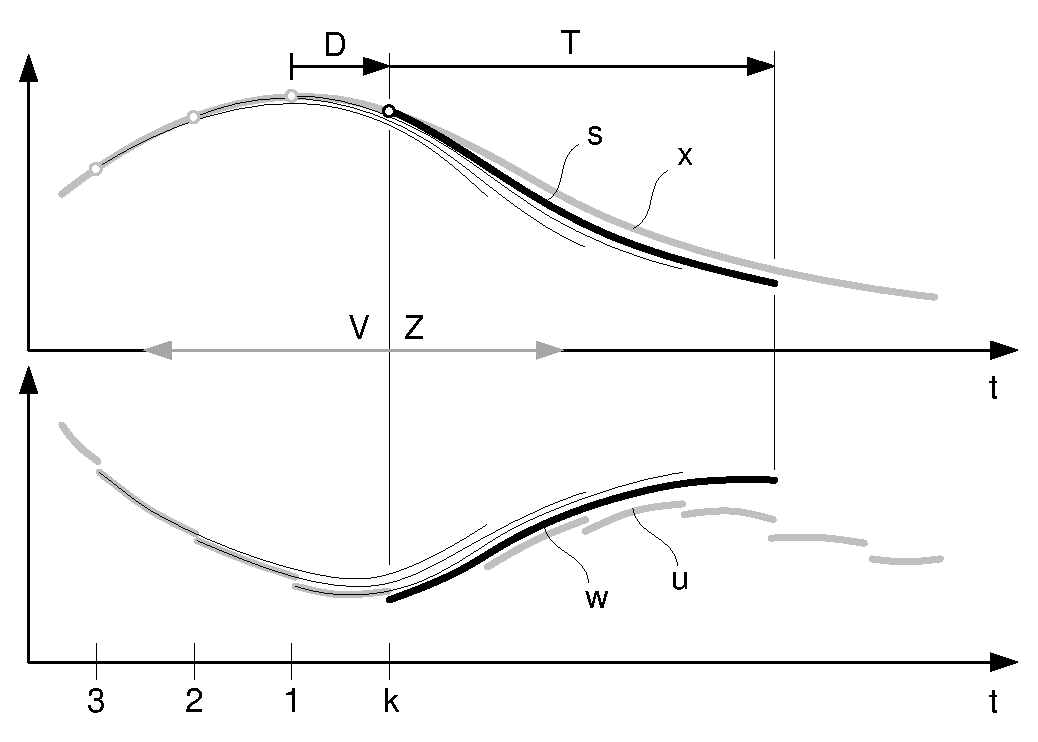
\includegraphics[width=1.\textwidth,clip, trim = 0cm 0cm 0cm 0cm]{2_mpc_grundidee_u_x.eps}
	\caption[Grundidee der modellprädiktiven Regelung]{Grundidee der modellprädiktiven Regelung; dick, schwarz: intern zum Zeitpunkt $t_k$ optimierte Zustands- und Stellgrößenverläufe; dünn, schwarz:  intern optimierte Verläufe der Vergangenheit; dick, grau: sich tatsächlich ergebende Verläufe des geschlossenen Regelkreises, vgl.\ \cite{graichen2014SkriptOpt}}
	\label{fig:2_mpc_grundidee_u_x}
\end{figure}

Mit dem Optimierungshorizont\index{Optimierungshorizont} $T$ und den darauf prädizierten Modellgrößen $\bar{\bs{x}}, \bar{\bs{u}}$ stellt sich das schritthaltend zu lösende Optimalsteuerungsproblem als
\begin{subequations} \label{equ:mpc_problem}
\begin{align}
	\underset{\bar{\bs{u}}(\cdot)}{\text{minimiere}}  \quad & %J(\bs{\phi}(t,\bar{\bs{u}}),\bs{\psi}(t,\bar{\bs{u}}),t)) = 
	\int_{t_k}^{t_k+T} l(\bar{\bs x}(\tau), \bar{\bs u}(\tau),\tau)\,{\rm d} \tau\,\,+\,\, V(\bar{\bs{x}}(t_k+T),t_k+T) \label{equ:mpc_funktional}\\
	\text{u.B.v.} \quad &\dot{\bar{\bs{x}}}(\tau) = \bs{f}(\bar{\bs{x}}(\tau),\bar{\bs{u}}(\tau),\tau), \quad \bar{\bs{x}}(t_k) = \bs{x}(t_k) \label{equ:mpc_system}\\\
\quad &\bs{g}(\bar{\bs{x}}(t_k+T),t_k+T) = \bs{0} \label{equ:mpc_gnb}\\ 	
	&\bs{h}(\bar{\bs{x}}(\tau),\bar{\bs{u}}(\tau),\tau) \leq \bs{0},  \quad \forall \tau \in[t_k, t_k + T] \label{equ:mpc_unb}
\end{align} 
\end{subequations}
dar. Aus Sicht der Optimierung gibt es keine algorithmischen Unterschiede zu \eqref{equ:optimalsteuerungsproblem}, weshalb sich die Kap.\,\ref{chap:dynamische_Optimierung_dynamisch}, \ref{chap:dynamische_Optimierung_direkt} und \ref{chap:dynamische_Optimierung_indirekt} auf das übersichtlichere Optimalsteuerungsproblem \eqref{equ:optimalsteuerungsproblem} beziehen. 

%\subsection{Systembeschreibung} \label{sec:direkte_methode_systembeschreibung}
%Nachstehend werden die verschiedenen Auslegungsmöglichkeiten der Bestandteile des Optimalsteuerungsproblems im Hinblick auf das Trajektorien-Optimierungsproblem auf Fahrzeugführungsebene beleuchtet und anhand von Literaturbeispielen aus dem Bereich des hochautomatisierten Fahrens und der Fahrerassistenz belegt. Wenn immer nötig werden hierbei, als Vorgriff auf die anschließenden Kapitel, Hinweise darauf gegeben, welchen Einfluss das angewendete Optimierungsverfahren hat. \\

% Inhalt:
% - Wahl der Zustandsgrößen abhängig von Optimierungsansatz
% - So wenige wie möglich, dass gerade noch so der Kern des Optimierungsproblems getroffenwird -> Hierarchische verbesserung
%


%Slackvariablen mit schönem Bild aus MPC
%\subsection{Einteilung der Lösungsmethodik} % ggf. nur überführende Bemerkung zu nächsten Kapitel, mit Anmerkung, dass zunächst noch Stabi. und Robustheit betrachtet wird.
% DP, dirO, indirO:
% DB: zeit- und wertdiskretes u (Anwendung)s
% dirO: zeitdiskretes u
% indir: kontinuierliche Verläufe

\section{Realisierbarkeits- und Stabilitätsbetrachtungen} \label{sec:stab_mpc}
Basiert der Regelkreis auf der Lösung eines Optimalsteuerungsproblems mit \emph{unendlich} langem Optimierungshorizont, dann weist er ganz besondere Eigenschaften auf. Insbesondere stimmen, in Abwesenheit von Störungen und Modellfehlern, in jedem Schritt die prädizierten Systemverläufe mit den tatsächlichen überein, was sich leicht mit dem später in Abschn.\,\ref{sec:bellman} vorgestellten \emph{Bellman'schen Optimalitätsprinzip} erklären lässt. Hiermit sichert die Lösbarkeit des Optimierungsproblems im Anfangszustand die Lösbarkeit für alle folgenden
Zeitschritte.
Dieser Sachverhalt wird in der Literatur auch als \emph{rekursive}\index{rekursive Lösbarkeit} oder \emph{anhaltende Lösbarkeit} (\emph{recursive}, \emph{persistent feasibility}) bezeichnet \cite{borrelli2014predictive, gruene2011nonlinear}. Des Weiteren garantiert ein unendlicher Optimierungshorizont unter recht allgemeinen Bedingungen \cite{borrelli2014predictive, gruene2011nonlinear, Findeisen2002} einen \emph{stabilen} Regelkreis, s.\ Abschn.\,\ref{sec:stabilität}. \\
Im Unterschied dazu beschränkt sich der modellprädiktive Regelkreis (aus Rechenzeitgründen) auf einen \emph{endlichen} Optimierungshorizont, der  
\iA zu einer \emph{Diskrepanz} zwischen den Lösungen der aufeinanderfolgenden Optimierungsschritte führt, s.\ Abb.\,\ref{fig:2_mpc_grundidee_u_x}. Die Hoffnung ist, dass sich die Einbußen der beschränkten Vorausschau in Bezug auf das Gütekriterium, aber auch auf die rekursive Lösbarkeit und die Stabilität in Grenzen halten. Wie nachfolgend anhand eines modellprädiktiven Abstandsregeltempomats (ACC) verdeutlicht wird, bewahrt die bloße Optimierung jedoch keinesfalls davor, dass sich der modellprädiktive Regelkreis in Situationen bringt, die nicht mehr lösbar sind, obwohl (anfänglich) eine Lösung für das Optimierungsproblem mit unendlichem Horizont existiert hat.
Wie ebenfalls simulativ verdeutlicht wird, ist die Stabilität des modellprädiktiven Regelkreises (selbst bei gegebener Lösbarkeit) nicht gesichert, sodass sich das geregelte System aufschwingen kann.
%Nachfolgend wird aufgrund der hochgradigen Relevanz der modellprädiktiven Regelung in der Fahrerassistenz für die beschriebene Problematik weiter sensibilisiert. 
Es existieren jedoch auf der Lyapunov-Stabilitätstheorie\index{Lyapunov-Stabilität} basierende MPC-Schemata \cite{borrelli2014predictive, gruene2011nonlinear, Findeisen2002}, die durch geeignete Modifikation der Optimierungskosten und Nebenbedingungen die rekursive Lösbarkeit und Stabilität garantieren. Ein recht allgemeiner und gleichzeitig gut auf Fahrerassistenzprobleme übertragbarer Ansatz wird vorgestellt und auf das ACC-Regelungsproblem gewinnbringend angewandt. 

\subsection{Beispiel modellprädiktiver Abstandsregeltempomat} \label{sec:mpc_acc}
Das Ziel eines Abstandsregeltempomaten\index{Abstandsregeltempomat} (\emph{Adaptive Cruise Control}, ACC) ist, eine vom Fahrer eingestellte Sollgeschwindigkeit einzuregeln (Tempomatfunktion), ohne dass ein vorgegebener Sollabstand zum vorausfahrenden Fahrzeug dauerhaft unterschritten wird. Eine Regelung mit unterschiedlichen Regelzielen wird auch als \emph{override control}\index{override control} bezeichnet \cite{glattfelder1983soc} und lässt sich im vorliegenden Fall dadurch realisieren, dass sich mittels
\begin{align*}
	u(\bs x) = \min(r_v(\bs x), r_d(\bs x))
\end{align*}
immer das stärker bremsende bzw.\ weniger starke beschleunigende Regelgesetz auf die Aktorik durchschlägt \cite{atSonderheft08, handbuchFAS_Winner}. Da für die Lösbarkeits- und Stabilitätsbetrachtungen das Abstandsregelgesetz $r_d(\bs x)$ von größerem Interesse ist als das Geschwindigkeitsregelgesetz $r_v(\bs x)$, wird auf ersteres eingegangen. Die Rückführung $r_d(\bs x)$ soll hier als modellprädiktiver Regler ausgeführt werden, dessen Optimierungskriterium \eqref{equ:mpc_funktional} sowie Fahrzeugmodell \eqref{equ:mpc_system} und die daran gestellten Ungleichungsnebenbedingungen \eqref{equ:mpc_unb} nachfolgend hergeleitet werden. Für die eigentliche Lösung der Optimierungsaufgabe muss jedoch auf die nachfolgenden Kapitel verwiesen werden.

\begin{figure}[h]
\centering
    \psfrag{A}[tc][tc][1.]{Ist-Position}
		%\psfrag{B}[tc][tc][1.]{\parbox[t]{3cm}{Soll-Position \\ ($\Delta x = 0$)}}
		\psfrag{B}[tc][tc][1.]{Soll-Position}
		\psfrag{C}[tc][tc][1.]{Vorderfahrzeug}
		\psfrag{D}[cc][cc][1.]{$\Delta x = 0$}
    \psfrag{1}[bc][bc][1.]{$v_v$}
		\psfrag{2}[bc][bc][1.]{$v_\text{ego}$}
		\psfrag{3}[bc][bc][1.]{$x_v$}
		\psfrag{4}[bc][bc][1.]{$x_\text{ego}$}
		\psfrag{5}[bc][bc][1.]{$d$}
	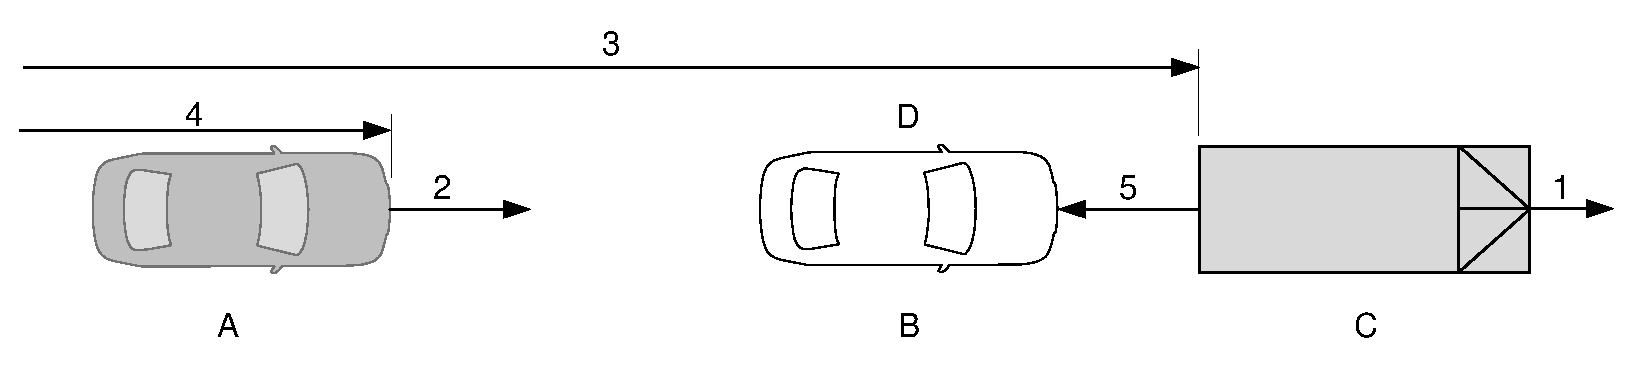
\includegraphics[width=1.\textwidth,clip, trim = 0cm 0cm 0cm 0cm]{3_ACC_topview.eps}
	\caption{Systemgrößendefinition der modellprädiktiven Abstandsregelung}
	\label{fig:ACC_topview}
\end{figure}

Es sei Abb.\,\ref{fig:ACC_topview} betrachtet, in der die Längsposition der Ego-Fahrzeugfront  $x_\text{ego}$ und des Vorderfahrzeughecks $x_v$ eingezeichnet sind. Da für die Funktion nur Relativgrößen von Belang sind, wird für das Systemmodell der Systemzustand $\Delta x =  x_\text{ego} - [x_v-d]$ eingeführt, der die Regelabweichung von der durch den Sollabstand $d$ definierten Sollposition $[x_v-d]$ beschreibt. Ist das Regelziel erreicht, dann befindet sich das Egofahrzeug, wie in Abb.\,\ref{fig:ACC_topview} in Weiß dargestellt, bei $\Delta x=0$.
Die zeitliche Änderung von $\Delta x$ wird wiederum von der relativen Annäherungsgeschwindigkeit $\Delta v = v_\text{ego} - v_v$ beschrieben. Vereinfachend gilt für die Vorderfahrzeuggeschwindigkeit $v_v = \text{const.}$ , d.h.\ der vorausfahrende Verkehr beschleunigt oder verzögert nicht\footnote{Abweichungen von diesem Verhalten stellen Störungen dar, die durch Modifikation des im Folgenden beschriebenen Herangehens behandelt werden können, vgl.\ \cite{dold2010robuste}.}.  Aus Komfortgründen muss die Ego-Längsbeschleunigung später im geschlossenen Regelkreis stetig verlaufen, was dadurch sichergestellt werden kann, dass sie als Systemzustand $a_\text{ego}$ aufgefasst wird, s.\ später hierzu auch Abb.\,\ref{fig:KR_Integrator_Erweiterung}. Insgesamt lässt sich damit die Annäherungsdynamik mit dem linearen, zeitinvarianten System 
%$\bs x = [\Delta x, \Delta v, a]$, $u$ Ruck
\begin{align}\label{equ:acc_sys}
	\dot{\bs x} = %\bs f(\bs x, u) = 
	\bs A \bs x + \bs b u \quad \text{mit} \quad \bs x = \mtrx{c}{\Delta x \\ \Delta v \\ a_\text{ego}} \!\! , \; \bs A = \mtrx{ccc}{0 & 1 & 0 \\ 0 & 0 & 1 \\ 0 & 0 & 0 } \text{und} \;\; \bs b = \mtrx{c}{ 0 \\ 0 \\ 1 }
\end{align}
beschreiben, wobei der Längsruck $j_\text{ego}=\dot a_\text{ego}(t)$ den Systemeingang $u$ darstellt. \\
Die von der Aufgabenstellung herrührenden zeitinvarianten Ungleichungsnebenbedingungen setzen sich aus der Kollisionsfreiheit mit dem Vorderfahrzeug $(\Delta x(t) \leq d)$ und dem beschränkten Beschleunigungs- und Verzögerungsvermögen $(a_{\min} \leq a(t) \leq a_{\max})$ zusammen, die sich %$\bs x = [x_1, x_2, x_3]^\T$
 kompakt als
%\begin{align*}
	%\bs g(\bs x) = \mtrx{c}{x_1 \\ x_3 \\ -x_3} \leq \mtrx{c}{d \\ a_{\max}  \\ -a_{\min}}
%\end{align*}
%
\begin{align} \label{equ:acc_unb}
	%\bs g(\bs x) = 
	\bs A_c \bs x - \bs b_c \leq \bs 0 \quad \text{mit} \quad \bs A_c = \mtrx{ccc}{1 & 0 & 0 \\ 0 & 0 & 1 \\ 0 & 0 & -1 } \text{und} \;\; \bs b_c = \mtrx{c}{ d \\ a_{\max}  \\ -a_{\min} }
\end{align}
darstellen lassen.

Schließlich werden die im Kostenfunktional \eqref{equ:mpc_funktional} des modellprädiktiven Reglers auftretenden Integralkosten in quadratischer Form zu
\begin{align}
	l(\bs{x},u) &= \bs x^\T \bs Q_\text{acc} \bs x + R_\text{acc} u^2 \quad \text{mit} \quad \bs Q_\text{acc} =  \bs Q_\text{acc}^\T > 0 \; \text{und} \; R_\text{acc} > 0 \label{equ:acc_integral}
	%V(\bs x(t_f)) &= \bs x(t_f)^\T \bs P \bs x(t_f) \quad \text{mit} \quad \bs P\succ 0 \;,
\end{align}
gewählt, sodass Abweichungen von der Sollposition $\Delta x = 0$ und deren zeitliche Ableitungen bestraft werden. Bei $\bs Q_\text{acc}$ handelt es sich somit um eine symmetrische, positiv definite\footnote{Eine Matrix $\bs A$ ist positiv definit, falls $\bs x^\T \bs A \bs x > \bs 0 \; \forall \bs x \in \mathbb R^n \setminus \{\bs 0\}$ und $\bs x^\T \bs A \bs x = \bs 0$ für $\bs x = \bs 0$; gilt anstelle des Vergleichsoperators $>$ nur $\geq$, so ist $\bs A$ positiv semidefinit. }  Matrix. Auf einen Endkostenterm $V(\bs x(t_f))$ in \eqref{equ:mpc_funktional} wird in einem ersten Ansatz zunächst verzichtet. \\
Mit \eqref{equ:acc_sys}, \eqref{equ:acc_unb} und \eqref{equ:acc_integral} ergibt sich für \eqref{equ:mpc_problem} ein sog.\ linear-quadratisches Optimierungsproblem (lineares Systemmodell, quadratisches Kostenfunktional) mit linearen Nebenbedingungen, das mit den später in Abschn.\,\ref{sec:direkte_einfach_schiessverfahren} beschriebenen Verfahren effizient gelöst werden kann. 
Damit wird der modellprädiktive Regelkreis geschlossen und aus der Streckendynamik $\dot{\bs x} = \bs f(\bs x, u)$ entsteht ein autonomes System $\dot{\bs x} = \bs f(\bs x, r_d(\bs x))$. Von der Umfeldsensorik neu erkannte Vorderfahrzeuge führen folglich zu Anfangsfehlern $\bs{x}_0$, die das System zu $\bs x_s = \bs 0$ abbauen muss, um den Sollabstand einzuregeln.

Die Optimierung erfolgt mit einer Zykluszeit von $\unit[100]{ms}$ und der Optimierungshorizont wird zunächst auf $T = \infty$ gesetzt\footnote{In guter Näherung wird in der numerischen Optimierung der Horizont auf $\unit[100.0]{s}$ begrenzt, da darüber hinaus keine nennenswerten Veränderungen in den Ergebnissen beobachtet werden können.}. In Abb.\,\ref{fig:3_MPC_Infeasable} ist das entsprechende Simulationsergebnis für einen um $\unitfrac[20]{m}{s}$ langsameren Einscherer\footnote{in die Ego-Spur wechselndes Vorderfahrzeug} dargestellt, der $\unit[25]{m}$ vor dem Ego-Fahrzeug erkannt wird, sodass die Situation ein drastisches Bremsen erfordert. Wie der hellgrauen 2d-Projektion entnommen werden kann, überführt der unendliche Optimierungshorizont das Fahrzeug von $\bs x_0 = [\unit[-15.0]{m}, \unitfrac[20.0]{m}{s}, \unitfrac[0.0]{m}{s^2}]$ in den Ursprung (Stern), sodass sich der Sollabstand von $d=\unit[10.0]{m}$ einstellt. Dabei werden zwei der Ungleichungsnebenbedingungen aktiv, wie später den hellgrauen Signalverläufen in Abb.\,\ref{fig:MPC_Signals} auf S.\,\pageref{fig:MPC_Signals} entnommen werden kann. Sie können aber zu jedem Zeitpunkt eingehalten werden, sodass weder die zulässige Verzögerung überschritten, noch das Vorderfahrzeug berührt werden. Aufgrund des Bellman'schen Optimalitätsprinzips folgt hierbei das System in jedem Schritt der zuvor optimierten Trajektorie, sodass in der Abbildung keine Diskrepanz zwischen geplanter und tatsächlicher Trajektorie erkennbar ist.

\begin{figure}[ht]
	%\centering
	% Erste Figure	
	\def\xlabel{$\Delta x$ in $\unit{m}$}
	\def\vlabel{$\Delta v$ in $\unitfrac{m}{s}$}	
	\def\alabel{$\mathcal{C}_\infty$}
	\def\blabel{ICS}
	\def\x0{$\bs x_0$}
	% Generated using matlabfrag
% Version: v0.6.16
% Version Date: 04-Apr-2010
% Author: Zebb Prime
%
%% <text>
%
\providecommand\matlabtextA{\color[rgb]{0.000,0.000,0.000}\fontsize{10}{10}\selectfont\strut}%
\psfrag{009}[cl][cl]{\matlabtextA \x0}%
\psfrag{010}[cl][cl]{\matlabtextA \blabel}%
\psfrag{011}[cl][cl]{\matlabtextA \alabel}%
\psfrag{012}[bc][bc]{\matlabtextA \vlabel}%
\psfrag{013}[tc][tc]{\matlabtextA \xlabel}%
%
%% </text>
%
%% <xtick>
%
\def\matlabfragNegXTick{\mathord{\makebox[0pt][r]{$-$}}}
%
\psfrag{000}[ct][ct]{\matlabtextA $\matlabfragNegXTick 20$}%
\psfrag{001}[ct][ct]{\matlabtextA $\matlabfragNegXTick 10$}%
\psfrag{002}[ct][ct]{\matlabtextA $0$}%
\psfrag{003}[ct][ct]{\matlabtextA $10$}%
%
%% </xtick>
%
%% <ytick>
%
\psfrag{004}[rc][rc]{\matlabtextA $-10$}%
\psfrag{005}[rc][rc]{\matlabtextA $0$}%
\psfrag{006}[rc][rc]{\matlabtextA $10$}%
\psfrag{007}[rc][rc]{\matlabtextA $20$}%
\psfrag{008}[rc][rc]{\matlabtextA $30$}%
%
%% </ytick>
	%\renewcommand{\matlabtextA}{\scriptsize}
	%\renewcommand{\matlabtextB}{\scriptsize}
    \subfigure[Rekursive Unlösbarkeit für $T=0.5 {\rm s}$]{
		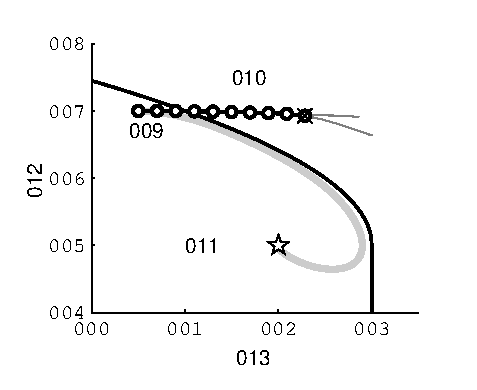
\includegraphics[width=.5 \linewidth,trim = 0cm 0cm 0cm 0cm]{3_MPC_Infeasable.eps}\label{fig:3_MPC_Infeasable}} %\\[3ex]
	% Zweite Figure	
	\def\dots{$(\ldots)$}
	\input{../Bilder/3_MPC_Instable.tex}
    \subfigure[Instabilität für $T=0.5 {\rm s}$]{
		\includegraphics[width=.5 \linewidth,trim = 0cm 0cm 0cm 0cm]{3_MPC_Instable.eps}
		\label{fig:3_MPC_Instable}}
	% Beschriftung
    \caption[Trajektorien des modellprädiktiven ACC-Regelkreises]{2d-Projektion der Trajektorien des modellprädiktiven Regelkreises; $T = \infty$ in Grau, $T=\unit[0.5]{s}$ mit weißen Punkten; Modellprädiktionen in dünnen, grauen Linien; $d = \unit[10.0]{m}$,
$a_{\min} = -\unitfrac[10.0]{m}{s^2}$,
$a_{\max} = \unitfrac[5.0]{m}{s^2}$,
$\bs Q_\text{acc} = \text{diag}(1,1,1)$,
$R_\text{acc} = 1$ (links), $R_\text{acc} = 5$ (rechts)}
\end{figure}

Ganz anders verhält sich ein auf $T = \unit[0.5]{s}$ reduzierter Optimierungshorizont. Aufgrund der kurzsichtigen Arbeitsweise nimmt die Optimierung erst nach $\unit[0.9]{s}$ Simulationszeit (neunter weißer Punkt in Abb.\,\ref{fig:3_MPC_Infeasable}) Notiz von der brenzligen Lage, sodass schon im zehnten Schritt keine Lösung des Optimalsteuerungsproblems mehr existiert (weißer Punkt mit Kreuz). Das verwundert nicht weiter, da sich das System  im vierten Schritt längst oberhalb der schwarzen Linie befindet, welche den Übergang zu der bereits in Abb.\,\ref{fig:ausweichen_vs_bremsen} auf S.\,\pageref{fig:ausweichen_vs_bremsen} abgebildeten ICS-Menge darstellt, den Zuständen einer unvermeidlichen Kollision. Die rekursive Lösbarkeit ist somit nicht gegeben und das Fahrzeug wird in der Realität kollidieren. \\
Ebenso wenig kann, selbst bei inaktiven Nebenbedingungen, die Stabilität des Regelkreises mit $T = \unit[0.5]{s}$ garantiert werden, wie dessen 2d-projizierte Systemtrajektorie in Abb.\,\ref{fig:3_MPC_Instable} verdeutlicht. Im Unterschied zur Regelung mit $T = \infty$ (hellgrau), die das System aus $\bs x_0 = [\unit[1.0]{m}, 0, 0]$ stabil in den Ursprung bringt, führt der kurze Optimierungshorizont zu einem Aufschwingen des Systems (weiße Punkte).

Zwar gibt es für bestimmte Problemklassen immer eine Grenze für $T$, oberhalb derer rekursive Lösbarkeit und Stabilität sichergestellt ist. Ihre Bestimmung ist jedoch mathematisch aufwändig \cite{graichen2014SkriptOpt} und überhaupt verbietet die verfügbare Rechenleistung häufig einen derart langen Optimierungshorizont. 
Um trotz eines kurzen Optimierungshorizonts ein gutes Ergebnis zu erzielen, existieren in der modernen Regelungstheorie Techniken, die Endkosten $V(\bs x(t_k\!+\!T), t_k\!+\!T)$ und Zielmengen für $\bs x(t_k\!+\!T) \in \mathcal{X}_f$ so vorgeben, dass der modellprädiktive Regler über den Optimierungshorizont hinaus auf das "`Kommende"' vorbereitet wird und Stabilität und rekursive Lösbarkeit gesichert sind. Wie sich bereits im ACC-Beispiel angekündigt hat, existieren hierbei Parallelen zu Methoden der Robotik, auch wenn dort die Stabilität typischerweise nicht im Fokus steht.

Nacheinander werden nun die wichtigsten Grundlagen geschaffen und in einem MPC-Schema kombiniert, das das Verhalten einer modellprädiktiven Regelung mit beschränktem Optimierungshorizont drastisch verbessert. Die Grundlagen und das Schema werden anhand des Abstandsregeltempomaten veranschaulicht.
%Das angewandte Konzept wird schließlich verallgemeinert, wobei Hinweise darauf gegeben werden, worin die Herausforderungen bei dessen praktischer Umsetzung bei zeitvarianten Systemen bestehen.

\subsection{Invariante Mengen\index{Invariante Menge}} \label{sec:invariantSets}
Der folgende Abschnitt bezieht sich wieder auf das Optimalsteuerungsproblem \eqref{equ:optimalsteuerungsproblem}. 
In vielen praktischen Aufgabenstellungen kann darin die sehr allgemeine Form \eqref{equ:opt_ungleichungen} der Ungleichungsbeschränkungen so abgewandelt werden, dass der Eingang $\bs u(t)$ und der Zustand $\bs x(t)$ nur noch unabhängig voneinander beschränkt sind und sich
\begin{alignat*}{2}
	{\bs x}(t) &\in \mathcal X \subseteq \mathbb R^n, & \quad {\bs u}(t) \in \mathcal U \subseteq \mathbb R^m; \quad \forall t &\in [t_0, t_f] %\\
	%\bar{\bs x}(\tau_f) &\in \mathcal X_f; & \quad \tau_f &= t_k + T
\end{alignat*}
schreiben lässt. %wobei $\mathcal X \subseteq \mathbb R^n$ und $\mathcal U\subseteq\mathbb R^m$ die Zustands- und Stellgrößenbeschränkungsmengen und $\mathcal X_f\subseteq \mathbb R^n$ die häufig als Endregion bezeichnete Zielmenge darstellen. 
In unmittelbarem Zusammenhang steht damit folgende Definition \cite{borrelli2014predictive}:

\begin{mydef}
Die Menge $\mathcal C \subseteq \mathcal X$ eines Systems \eqref{equ:opt_systemdynamik} mit Zustands- und Stellgrößenbeschränkungsmenge $\mathcal X, \mathcal U$ wird  als \emph{control-invariant} bezeichnet, wenn
\begin{align*}
	\bs x(0) \in \mathcal C \,\,  \Rightarrow \,\,  \exists \bs u(t) \in \mathcal U, \,\text{sodass} \, \bs x(t) \in \mathcal C \, ,\forall t \geq 0 
\end{align*}
gilt.
\end{mydef}
Für jedes Element der invarianten Zustandsmenge $\mathcal C$ gibt es also ein Stellgrößensignal $\bs u(t)$, sodass die Trajektorie $\bs x(t)$ die Zustandsmenge $\mathcal C$ nie verlässt.

% Falcone Threat ass. (11)
Wird der Systemzustand von \eqref{equ:opt_systemdynamik} mit einem Regler $\bs u = \bs r(\bs x)$ auf die Stellgröße rückgeführt, so entsteht wie im vorherigen Abschnitt ein \emph{autonomes} System. Existieren für die Regelstrecke Stellgrößenbeschränkungen, so werden sie im autonomen System Teil der Zustandsgrößenbeschränkung $\mathcal X$.
Ein autonomes System besitzt definitionsgemäß keinen Eingang, womit sich die Invarianz-Definition \cite{borrelli2014predictive} entsprechend vereinfacht:

\begin{mydef}
Für ein autonomes System $\dot {\bs x} = \bs f(\bs x)$ mit Zustandsbeschränkungsmenge $\mathcal X$ wird eine Menge  $\mathcal O \subseteq \mathcal X$ als \emph{positiv invariant} bezeichnet, wenn
\begin{align*}
	\bs x(0) \in \mathcal O \,\,  \Rightarrow \,\,  \bs x(t) \in \mathcal O, \, \forall t \geq 0 
\end{align*}
gilt. 
\end{mydef}
Demnach bleibt jede Trajektorie mit Anfangszustand in der invarianten Menge $\mathcal O$ für alle Zeit darin.

\begin{mydef}
Die \emph{Vereinigung} aller invarianten Mengen eines Systems wird als \emph{maximale invariante Menge} $\mathcal C_{\infty}$ \bzw  $\mathcal O_{\infty}$ bezeichnet \cite{borrelli2014predictive}. %
\end{mydef}

Aufgrund der linearen, zeitinvarianten Fahrzeuglängsdynamik \eqref{equ:acc_unb} gepaart mit den linearen Ungleichungsnebenbedingungen \eqref{equ:acc_unb} für $\mathcal X \subset \mathbb R^3$ lässt sich durch zeitliche Diskretisierung die maximale invariante Menge $\mathcal C_{\infty} \subset \mathcal X$ des ACC-Problems effizient mittels \cite{herceg2013multi} berechnen. Das Ergebnis ist in Abb.\,\ref{fig:C_inf_und_O_inf_LQR} als durchsichtiges Drahtgittermodell dargestellt, das bei $\Delta x = -\unit[150]{m}$ und $\Delta v = -\unitfrac[15]{m}{s}$ gestutzt wurde, da es sich aufgrund der Abwesenheit von Nebenbedingungen in diese Richtungen bis ins Unendliche fortsetzt. 
Eine bei $a_\text{ego} = 0\, \unitfrac{m}{s^2}$ entnommene Scheibe ist daneben in Abb.\,\ref{fig:MPC_Konvergenz} abgebildet. Auch hier sei darauf hingewiesen, dass aus Darstellungsgründen die Mengen zusätzlich zu den vorherigen Grenzen auch oberhalb von $\unitfrac[60]{m}{s}$ abgeschnitten sind. Aus der Abbildung
wird sofort der Zusammenhang
\begin{align}
	\mathcal C_\infty = \mathcal X \setminus \text{ICS}
\end{align}
ersichtlich. Die maximale invariante Menge $\mathcal C_\infty$ beinhaltet nämlich alle Zustände, die durch ein Stellgesetz überhaupt vor einer Verletzung der Nebenbedingung bewahrt werden können. Außerhalb führen alle Zustände %$\bs x\in \mathcal X$ 
zu einer Verletzung der Nebenbedingung, wie auch immer $u(t)$ gewählt wird, und liegen damit in der ICS-Menge, kollidieren also im Beispiel unweigerlich mit dem Vorderfahrzeug. 

\begin{figure}[ht]
	%\centering
	% Erste Figure	
	\def\xlabel{$\Delta x$ in $\unit{m}$}
	\def\vlabel{$\Delta v$ in $\unitfrac{m}{s}$}	
	\def\alabel{$a_\text{ego}$ in $\unitfrac{m}{s^2}$}	
	% Generated using matlabfrag
% Version: v0.6.16
% Version Date: 04-Apr-2010
% Author: Zebb Prime
%
%% <text>
%
\providecommand\matlabtextA{\color[rgb]{0.000,0.000,0.000}\fontsize{10}{10}\selectfont\strut}%
\psfrag{012}[bc][bc]{\matlabtextA \alabel}%
\psfrag{013}[tr][tr]{\matlabtextA \vlabel}%
\psfrag{014}[tl][tl]{\matlabtextA \xlabel}%
%
%% </text>
%
%% <xtick>
%
\def\matlabfragNegXTick{\mathord{\makebox[0pt][r]{$-$}}}
%
\psfrag{000}[ct][ct]{\matlabtextA $\matlabfragNegXTick 150$}%
\psfrag{001}[ct][ct]{\matlabtextA $\matlabfragNegXTick 100$}%
\psfrag{002}[ct][ct]{\matlabtextA $\matlabfragNegXTick 50$}%
\psfrag{003}[ct][ct]{\matlabtextA $0$}%
%
%% </xtick>
%
%% <ytick>
%
\psfrag{004}[rc][rc]{\matlabtextA $0$}%
\psfrag{005}[rc][rc]{\matlabtextA $20$}%
\psfrag{006}[rc][rc]{\matlabtextA $40$}%
\psfrag{007}[rc][rc]{\matlabtextA $60$}%
%
%% </ytick>
%
%% <ztick>
%
\psfrag{008}[cr][cr]{\matlabtextA $-10$}%
\psfrag{009}[cr][cr]{\matlabtextA $-5$}%
\psfrag{010}[cr][cr]{\matlabtextA $0$}%
\psfrag{011}[cr][cr]{\matlabtextA $5$}%
%
%% </ztick>
	%\renewcommand{\matlabtextA}{\scriptsize}
	%\renewcommand{\matlabtextB}{\scriptsize}
    \subfigure[Invariante Mengen]{
		\includegraphics[width=.55 \linewidth,trim = 0cm 0cm 0cm 0cm]{3_C_inf_und_O_inf_LQR.eps}\label{fig:C_inf_und_O_inf_LQR}} %\\[3ex]
		\!\!\!\!\!\!\!\!\!\!\!\!
	% Zweite Figure	
	%\def\xlabel{$x$ in $\unit{m}$}
	%\def\vlabel{$v$ in $\unitfrac{m}{s}$}
	\def\alabel{$\mathcal{C}_\infty$}
	\def\blabel{$\mathcal{O}_\infty^{\text{\tiny LQR}}$}
	\def\clabel{$\mathcal{O}_\infty^{0.5}$}
	\def\dlabel{$\mathcal{O}_\infty^{1.0}$}
	\def\elabel{ICS}
	\def\flabel{$\mathcal{X}$}
	% Generated using matlabfrag
% Version: v0.6.16
% Version Date: 04-Apr-2010
% Author: Zebb Prime
%
%% <text>
%
\providecommand\matlabtextA{\color[rgb]{0.000,0.000,0.000}\fontsize{10}{10}\selectfont\strut}%
\psfrag{012}[cl][cl]{\matlabtextA \flabel}%
\psfrag{013}[cl][cl]{\matlabtextA \elabel}%
\psfrag{014}[cl][cl]{\matlabtextA \dlabel}%
\psfrag{015}[cl][cl]{\matlabtextA \clabel}%
\psfrag{016}[cl][cl]{\matlabtextA \blabel}%
\psfrag{017}[cl][cl]{\matlabtextA \alabel}%
\psfrag{018}[bc][bc]{\matlabtextA \vlabel}%
\psfrag{019}[tc][tc]{\matlabtextA \xlabel}%
%
%% </text>
%
%% <xtick>
%
\def\matlabfragNegXTick{\mathord{\makebox[0pt][r]{$-$}}}
%
\psfrag{000}[ct][ct]{\matlabtextA $\matlabfragNegXTick 150$}%
\psfrag{001}[ct][ct]{\matlabtextA $\matlabfragNegXTick 100$}%
\psfrag{002}[ct][ct]{\matlabtextA $\matlabfragNegXTick 50$}%
\psfrag{003}[ct][ct]{\matlabtextA $0$}%
%
%% </xtick>
%
%% <ytick>
%
\psfrag{004}[rc][rc]{\matlabtextA $-10$}%
\psfrag{005}[rc][rc]{\matlabtextA $0$}%
\psfrag{006}[rc][rc]{\matlabtextA $10$}%
\psfrag{007}[rc][rc]{\matlabtextA $20$}%
\psfrag{008}[rc][rc]{\matlabtextA $30$}%
\psfrag{009}[rc][rc]{\matlabtextA $40$}%
\psfrag{010}[rc][rc]{\matlabtextA $50$}%
\psfrag{011}[rc][rc]{\matlabtextA $60$}%
%
%% </ytick>
    \subfigure[2d-Scheibe mit $a_\text{ego} = 0\, \unitfrac{m}{s^2}$]{
		\includegraphics[width=.5 \linewidth,trim = 0cm 0cm 0cm 0cm]{3_MPC_Konvergenz.eps}
		\label{fig:MPC_Konvergenz}}
	% Beschriftung
    \caption[Invariante Mengen für das ACC-Beispiel]{Invariante Mengen: ungeregeltes System $\mathcal C_\infty$ in Transparent/Weiß, LQR-geregeltes System $\mathcal{O}_\infty^{\text{\tiny LQR}}$ in Grau; durch Sampling bestimmter Einzugsbereiche $\mathcal{O}_\infty^{0.5}$ mit dunkelgrauen, kleinen Kästen und $\mathcal{O}_\infty^{1.0}$ mit hellgrauen, großen Kästen}
\end{figure}

Als Nächstes sei die Fahrzeuglängsdynamik über einen (stabilisierenden) Zustandsregler 
\begin{align}
	u(t)=\bs k_\text{LQR} \cdot \bs x(t) \label{equ:lqr}
\end{align}
mit noch zu spezifizierendem Verstärkungsvektor $\bs k_\text{LQR}^\T \in \mathbb R^3$ geschlossen. Die maximale invariante Menge des so entstehenden linearen autonomen Systems $\dot{\bs x} = [\bs A + \bs B \bs k_\text{LQR}] \bs x$, im Folgenden als $\mathcal{O}_\infty^{\text{\tiny LQR}}$ bezeichnet, kann ebenfalls problemlos berechnet werden und ist in Abb.\,\ref{fig:C_inf_und_O_inf_LQR} in transparentem Grau dargestellt. Jeder Anfangszustand auf dem Rand von $\mathcal{O}_\infty^{\text{\tiny LQR}}$ führt also dazu, dass auf dem Weg der Trajektorie in den Ursprung mindestens eine Nebenbedingung in einem Zeitpunkt in Gleichheit erfüllt ist. Alle Systemzustände außerhalb der Menge verletzen die Ungleichungsnebenbedingungen, bremsen oder beschleunigen demnach über Gebühr oder kollidieren mit dem Vorderfahrzeug.\\
Das Regelungsgesetz führt zu einem stetigen Beschleunigungsverlauf, sodass es nicht verwundert, dass sich $\mathcal{O}_\infty^{\text{\tiny LQR}}$ mit höheren Anfangsbeschleunigungen (in Abb.\,\ref{fig:C_inf_und_O_inf_LQR} nach oben hin) verkleinert, da es etwas Zeit braucht, bis wirklich verzögert wird.
Darüber hinaus ist erkennbar, dass die invariante Menge $\mathcal{O}_\infty^{\text{\tiny LQR}}$ des linearen Zustandsreglers bei Weitem unterhalb der "`Möglichkeiten"' der maximalen invarianten Menge $\mathcal{C}_\infty$ der Strecke bleibt, viele Zustände also zu Kollisionen führen, die grundsätzlich verhindert werden könnten. Die maximal positiv invariante Menge des später vorgestellten modellprädiktiven Reglers stellt sich deutlich größer dar.

%Es gilt dahier immer $\mathcal O_\infty \subseteq \mathcal C_\infty$


	
	\subsection{Lyapunov-Stabilität\index{Lyapunov-Stabilität}} \label{sec:stabilität}
	Im Unterschied zur Robotik spielt in der Regelungstechnik  der Nachweis der Systemstabilität eine zentrale Rolle. Für die Praxis reicht es \iA hierbei nicht aus, asymptotische Konvergenz $\lim_{t\rightarrow \infty} \bs x(t)= \bs 0$ für den geschlossenen Regelkreis zu zeigen. Vielmehr soll auch sichergestellt werden, dass sich das (geregelte) System bei kleinen Störungen gutmütig verhält und in der Nähe des Ursprungs bleibt. Diese  Eigenschaft wird in folgendem Stabilitätsbegriff formalisiert \cite{khalil2002nonlinear} und in Abb.\,\ref{fig:delta_epsilon} veranschaulicht.
%Stabilitätskriterium, das auch im nichtlinearen funktioniert.

\begin{figure}[ht]
\centering
    \psfrag{1}[tc][tc][1.]{$x_1$}
		\psfrag{2}[lc][lc][1.]{$x_2$}
		\psfrag{0}[lb][lb][1.]{$\bs x_0$}
		\psfrag{d}[rb][rb][1.]{$\delta$}
		\psfrag{e}[rb][rb][1.]{$\varepsilon$}
		\subfigure[Lyapunov-Stabilität]{
		\includegraphics[width=.4 \linewidth,trim = 0cm 0cm 0cm 0cm]{3_delta_epsilon.eps}\label{fig:delta_epsilon}}
		%\psfrag{V}[rb][rb][1.]{$\frac{\partial}{\partial \bs x} V(\bs x)$}
		\hspace{.5cm}
		\psfrag{f}[cc][cc][1.]{$\bs f(\bs x)$}
		\psfrag{V}[cc][cc][1.]{$\frac{\partial}{\partial \bs x} V(\bs x)$}
		\psfrag{C}[tl][tl][1.]{$V(\bs x)\!=\!\text{const.}$}
		\subfigure[Lyapunov-Funktion]{
		\includegraphics[width=.4 \linewidth,trim = 0cm 0cm 0cm 0cm]{3_Lyap_Funktion.eps}\label{fig:Lyap_Funktion}} 
	\caption[Veranschaulichung von Stabilitätsdefinition und -kriterium]{Veranschaulichung von Stabilitätsdefinition und -kriterium \cite{khalil2002nonlinear}}
	\label{fig:3_delta_epsilon}
\end{figure}

\begin{mydef}
Der stationäre Punkt $\bs x_s = \bs 0$ des autonomen Systems
	$ \dot {\bs x} = \bs f(\bs x) $
ist \emph{stabil} im Sinne von Lyapunov, wenn für jedes (noch so kleine) $\varepsilon > 0$ ein $\delta > 0$ %$\delta(\varepsilon)$ 
existiert, sodass %für jedes $\bs x_0 \in \mathcal X$
\begin{align*}
	\|\bs x_0 \| < \delta \Rightarrow \| \bs x(t)\| < \varepsilon, \forall t \geq 0 \;.
\end{align*}
Gilt zudem $\lim_{t\rightarrow \infty} \bs x(t)= \bs 0, \forall \bs x(0)\in \Omega$, so ist das System auf dem Gebiet $\Omega\in\mathbb R^n$ \emph{asymptotisch stabil}.
% S. https://www.kirp.chtf.stuba.sk/pc11/data/workshops/mpc/MPC_PC11_Lecture1.pdf -> S. 21
\end{mydef}

Für die Stabilitätsuntersuchung nichtlinearer Systeme, und hierzu zählt auch der modellprädiktive Regelkreis aufgrund seines aufwändigen Rückführungsgesetzes, eignet sich die sog.\ \emph{direkte Methode von Lyapunov} \cite{khalil2002nonlinear}:

\begin{satz} \label{theo:lyapunovstab}
Es sei $\mathcal D \subseteq\mathbb R^n$ eine offene Umgebung von $\bs x_s = \bs 0$. Existiert eine Funktion $V(\bs x):\mathcal D \rightarrow \mathbb R$, sodass %für $V(\bs x)$ auf $\mathcal D$ 
\begin{subequations}
\begin{align}
	V(\bs 0) &= 0; \quad \,\, V(\bs x) > 0, \,\, \forall \bs x \in \mathcal D \setminus\{\bs 0\} \label{equ:lyap_V}\\
%\end{align*}
%und
%\begin{align*}
	\dot V(\bs x) &= \frac{\partial }{\partial \bs x} V(\bs x)\bs f(\bs x) \leq - \alpha(\bs x), \,\, \forall \bs x \in \mathcal D \setminus\{\bs 0\} \, , \label{equ:lyap_V_dot}
\end{align}
\end{subequations}
wobei es sich bei $\alpha : \mathbb R^n \rightarrow \mathbb R$ um eine stetige positiv definite Funktion handelt, dann ist $\bs x_s=\bs 0$ auf $\mathcal D$ asymptotisch stabil, und $V(\bs x)$ wird Lyapunov-Funktion genannt.
\end{satz}
% abgewandelt aus
% MPC-Book

Bei der skalaren Lyapunov-Funktion $V(\bs x)$  handelt es sich um eine Energiefunktion im erweiterten Sinne: Sie ist nur Null im Ursprung, sonst positiv, s.\ \eqref{equ:lyap_V}, und muss über der Zeit stets abnehmen bis der Ursprung erreicht ist, s.\ \eqref{equ:lyap_V_dot}. %, damit $\dot{\bs x} = \bs f(\bs x)$ stabil ist. 
Die Existenz einer solchen Energiefunktion ist dann hinreichend dafür, dass $\bs x_s = \bs 0$ stabil im Sinne von Lyapunov ist, s.\ \zB \cite{khalil2002nonlinear}.
Zur Interpretation von \eqref{equ:lyap_V_dot} sei Abb.\,\ref{fig:Lyap_Funktion} betrachtet, worin die Höhenlinien von $V(\bs x)$ in unterschiedlichen Grautönen dargestellt sind. \\
Bei Anwendung des Stabilitätskriteriums auf Regelkreise werden $V(\bs x)$ als \emph{Control-Lyapunov-Funktion} (CLF) und die Rückführung  $\bs r(\bs x)$ als \emph{CLF-Reglergesetz} bezeichnet.

Das Stabilitätskriterium wird nun auf den zuvor durch die lineare ACC-Zustandsregelung \eqref{equ:lqr} geschlossenen Regelkreis angewandt, wobei die Ergebnisse ebenfalls für den späteren Entwurf einer leistungsstarken modellprädiktiven Regelung von Interesse sind. Die Zustandsrückführung wird nämlich optimal im Sinne eines LQR-Entwurfs \cite{lunze2012regelungstechnik} ausgelegt, der kurz erläutert werden soll.
\begin{mydef}
Ein sog.\ \emph{Linear Quadratic Regulator}\index{Linear Quadratic Regulator} (LQR) minimiert für ein lineares, zeitinvariantes System 
\begin{align}
 \dot{\bs x} = \bs A \bs x + \bs B \bs u, \quad \bs x(t) \in \mathbb R^n, \bs u(t) \in \mathbb R^m \label{equ:lq_problem_f}
\end{align}
das Kostenfunktional 
\begin{align*}
 J = \int_{t_0}^{\infty} [\bs x^\T \bs Q \bs x + \bs u^\T \bs R \bs u ]\,{\rm d} t \;. %\label{equ:lq_problem_J}
\end{align*}
\end{mydef}
Es wird hierbei auf den \emph{unendlichen} Optimierungshorizont hingewiesen. 
Der Einfachheit halber seien beide symmetrischen Wichtungsmatrizen $\bs Q=\bs Q^\T$ und $\bs R=\bs R^\T$ wie im ACC-Beispiel positiv definit\footnote{
Falls der allgemeine Fall einer positiv semidefiniten Matrix $\bs Q$ betrachtet werden soll, so ist der nachfolgende Stabilitätsbeweis für asymptotische Stabilität etwas aufwändiger.}. Es gilt folgender Satz \cite{graichen2014SkriptOpt}:
%
\begin{satz} \label{theo:lqr_stab}
Falls $\bs Q$ und $\bs R$ symmetrisch und positiv definit sowie $(\bs A,\bs B)$ stabilisierbar und $(\bs A,\bs M)$ mit $\bs Q = \bs M^\T \bs M$ entdeckbar sind, dann lautet das optimale Rückführgesetz
\begin{align}
\bs u(t) = \bs r(\bs x(t)) = -\bs R^{-1} \bs B^\T \bs P \, \bs x(t) = -\bs K_\text{LQR} \,\bs x(t) \;,   \label{equ:riccati_alg_u}
\end{align}
wobei $\bs P$ die eindeutige, symmetrische, positiv semidefinite Lösung der algebraischen Matrix-Riccati-Gleichung 
\begin{align}
\bs P \bs B \bs R^{-1} \bs B^T \bs P - \bs P \bs A - \bs A^T \bs P - \bs Q = \bs 0 \label{equ:riccati_alg}
\end{align}
darstellt. Die Ruhelage $\bs x_s = \bs 0$ des hierdurch geschlossenen Regelkreises ist asymptotisch stabil. \\
\end{satz}
Für die Herleitung von \eqref{equ:riccati_alg_u} und \eqref{equ:riccati_alg} wird auf Abschn.\,\ref{sec:riccati_dgl} verwiesen. Auch ohne sie kann auf Basis von Satz~\ref{theo:lyapunovstab} bereits die behauptete Stabilität gezeigt werden:

Mit dem Lyapunov-Funktionskandidaten
\begin{align}
	V(\bs x) = \bs x^\T \bs P \bs x \label{equ:lyap_lqr}
\end{align}
ergibt sich
\begin{align*}
	\dot V(\bs x) &= \dot{\bs x}^\T \bs P \bs x + \bs x^\T \bs P \dot{\bs x} \\
	&= [\bs x^\T \bs A^\T + \bs u^\T \bs B^\T]\bs P \bs x + \bs x^\T \bs P[\bs A \bs x + \bs B \bs u]
\end{align*}
und mit \eqref{equ:riccati_alg_u} und \eqref{equ:riccati_alg} gilt damit
\begin{align}
\nonumber
	\dot V(\bs x) &= \bs x^\T \bs A^\T \bs P \bs x  -\bs x^\T \bs P \bs B \bs R^{-1} \bs B^\T
	\bs P \bs x + \bs x^\T \bs P \bs A \bs x - \bs x^\T \bs P \bs B \bs R^{-1} \bs B^\T \bs P \bs x \\
\nonumber
	&= 	\bs x^\T [ \underbrace{\bs A^\T \bs P  -\bs P \bs B \bs R^{-1} \bs B^\T
	\bs P + \bs P \bs A}_{-\bs Q}] \bs x - \bs x^\T\bs P \bs B \bs R^{-1} \bs B^\T \bs P \bs x \\
	&= \underbrace{-\bs x^\T \bs Q \bs x}_{\leq 0} \quad \underbrace{- \bs x^\T \bs P \bs B \bs R^{-1} \bs B^\T \bs P \bs x}_{\leq 0} \quad \leq 0\;. \label{equ:V_dot_alg} 
\end{align}
Damit ist der Regelkreis auf $\mathbb R^n$ asymptotisch stabil.

Wird der ACC-Zustandsregler \eqref{equ:riccati_alg_u} auf Basis der Wichtungsmatrizen $\bs Q_\text{acc}$ und $R_\text{acc}$ in \eqref{equ:acc_integral} entsprechend Satz~\ref{theo:lqr_stab} entworfen, dann stabilisiert er asymptotisch die Ruhelage $\bs x_s = \bs 0$ "`per Design"'. Eine gesonderte Stabilitätsuntersuchung des Regelkreises, etwa durch Betrachtung dessen Pole, ist überflüssig. 
Wie in Abschn.\,\ref{sec:invariantSets} bereits dargelegt, reduziert sich das Einzugsgebiet $\mathcal D$ jedoch durch die Ungleichungsnebenbedingungen auf die maximal positiv invariante Menge $\mathcal{O}_\infty^{\text{\tiny LQR}}$.  

Die Lyapunov-Funktion \eqref{equ:lyap_lqr} kann anschaulich interpretiert werden, denn sie stellt die optimale Kostenfunktion $J^\ast(\bs x)$ dar. Auch die MPC-Schemata basieren auf den Kosten $J^\ast(\bs x)$ als Lyapunov-Funktion, um eine Stabilitätsgarantie aussprechen zu können.

% http://www.acin.tuwien.ac.at/fileadmin/cds/lehre/rsys/Archiv/Skriptum_Regelungssysteme_SS2011.pdf S.49

% 2) Wichtigstes Standardherangehen aus Regelungstechnik, konstruktiv, sodass MPC besser wird
% 3) Schwierigkeiten bei zeitvarianten Nebenbedingungen und gar bei zeitveränderlicher Umgebung

% Wichtige Punkte:
% - Als Systemeingang darf nicht u herangezogen werden, sondern die zu optimierenden Parameter wg. Approximation
% - Ausblick darauf, dass Optimierung nicht ganz abgeschlossen werden muss, um stabil zu sein, solange die Lyapunov-Funktion weiter abnimmt (Suboptimale Regelung)
% Es existiert immer ein hinreichend langer Horizont, sodass das System stabil ist. (gilt sicherlich nicht für zeitinvariante Probleme)

% Zu diskutierende Thesen: 
% Maximale control-invariante Menge (C_inf) = inv(ICS)  ?
% Zielmenge C_inf reicht nicht für persistent feasibility (anhaltende Realisierbarkeit) ? Begründung: Nur weil es eine Lösung gibt, heißt das nicht, dass ein Algorithmus, der auf einem endlichen Horizont optimiert, diese (in zeitlich aufeinanderfolgenden Schritten) findet.
% Was bringt mir dann die ICS-Menge?
% Was kann für zeitvariante NB abgeleitet werden?

% TODO: Hinweis darauf, dass bei LQ-Problemen sich Quadratisches Programm ergibt, das nicht numerisch approximiert werden muss und in einem Schritt gelöst werden kann.




% Vereinfachungen: Zeitvariante NB ändern sich nicht von Problem zu problem. 
% Was kann schief gehen: no feasibiltiy -> plötzlich keine Kollisionsfreie Traj, no stability: system schwing sich auf und nichtmodellierte Dynamiken werden angesprochen, sodass das System von der Straße abkommt.
%H. Chen und F. Allgower. A quasi-infinite horizon nonlinear model predictive control scheme with guaranteed stability. Automatica, 34(10):1205{1217, 1998.

% Kurze übersicht, auch invarianzregelung: https://www.kirp.chtf.stuba.sk/pc11/data/workshops/mpc/MPC_PC11_Lecture1.pdf

%Für einen endlich langen Optimierungshorizont muss der Endzustand in einer Invarianten Menge liegen, für die ein invarianz-induzierter Regler existiert, dessen Kosten auf einem unendlichlangen Horizont in geschlossener Form dargestllt werden kann. --> Lierfert Endbedingung und Enkosten, Regler wird aber nie verwendet!



%\subsection{Unendlicher Optimierungshorizont} \label{sec:infinit_horizon_mpc}
% es gibt eine obere schranke für den optimierungshorizont für die stabilität garantiert ist. Eher für die Simulation interessant. Erweiterung für zielmenge und endkosten aber für fahrzeuganwendung nicht tragisch, da problem nur unwesentlich komplizierter wird -> nächster Abschnitt

%If problem is feasible, the closed loop trajectories will be always feasible, If the cost is finite, then states and inputs will converge asymptotically to the origin [Folien Morari 5-30]
\subsection{MPC-Schema mit Garantien} %Endlicher Optimierungshorizont mit Zielregion} \label{sec:finite_horizon_mpc}
% Stabilitätsnachweis über Endzustand nicht möglich, da ggf. Endzustand nicht frei
% Optimalsteuerungsproblem definieren
% Fahrzeugmodelle + Ungebung -> gütekriterium + nebenbediunng
% Erklärung Lyapunov-Stabilität
% Trajektorienplanung für Fahrzeug: Optimierung auf endlichem Horizont ->
% Stabilität
Ein sehr weit verbreiteter MPC-Ansatz, der sich gut mit den Anforderungen der Fahrerassistenz vereinbaren lässt, basiert darauf, durch Vorgabe bestimmter Endkosten $V$ und einer Zielregion $\mathcal X_f$
%\begin{align*}
 %\bar{\bs x}(\tau_f) &\in \mathcal X_f; & \quad \tau_f &= t_k + T
%\end{align*}
für den Endzustand $\bar{\bs x}(t_k + T)$ die rekursive Lösbarkeit und Stabilität sicherzustellen. 
%Introduce terminal cost and constraints to explicitly ensure stability and feasibility:!
%https://www.kirp.chtf.stuba.sk/pc11/data/workshops/mpc/MPC_PC11_Lecture1.pdf
%
Für ein zeitinvariantes Problem stellt sich dann das schritthaltend zu lösende Optimalsteuerungsproblem als
\begin{subequations} \label{equ:mpc_problem_zeitinvariant}
\begin{align}
	\underset{\bar{\bs{u}}(\cdot)}{\text{minimiere}}  \quad & J(\bs x(t_k), \bar{\bs u}) =%J(\bs{\phi}(t,\bar{\bs{u}}),\bs{\psi}(t,\bar{\bs{u}}),t)) = 
	\int_{t_k}^{t_k+T} \!\!l(\bar{\bs x}(\tau), \bar{\bs u}(\tau))\,{\rm d} \tau\,\,+\,\, V(\bar{\bs{x}}(t_k+T)) \label{equ:mpc_funktional_inv}\\
	\text{u.B.v.} \quad &\dot{\bar{\bs{x}}}(\tau) = \bs{f}(\bar{\bs{x}}(\tau),\bar{\bs{u}}(\tau)), \quad \bar{\bs{x}}(t_k) = \bs{x}(t_k) \label{equ:mpc_system_inv}\\
	& \bar{\bs{x}}(\tau) \in \mathcal X, \quad \bar{\bs{u}}(\tau) \in \mathcal U, \quad \forall \tau \in[t_k, t_k + T] \label{equ:mpc_unb_Xf} \\
	& \bar{\bs x}(t_k + T)  \in \mathcal X_f%, \quad  \bar{\bs x}_f = \bar{\bs x}(t_k + T) \bar{\bs{x}}_f
\end{align} 
\end{subequations}
dar.

Der folgende Satz macht, unter recht milden Zusatzannahmen \cite{graichen2014SkriptOpt, gruene2011nonlinear}, eine Aussage darüber, wann \eqref{equ:mpc_problem_zeitinvariant} rekursiv lösbar und der modellprädiktive Regelkreis stabil ist:
\begin{satz}\label{theo:mpc_zielmenge}
Die Menge $\mathcal X_0 \subseteq \mathcal X \subseteq \mathbb R^n$ bezeichne die nichtleere Menge aller Anfangsbedingungen $\bs x(t_k)$, für die \eqref{equ:mpc_problem_zeitinvariant} lösbar ist.
Weiter existiert eine kompakte nichtleere Menge $\mathcal X_f=\{ \bs x \in \mathbb R^n : V(\bs x) \leq \beta \} \subseteq \mathcal X_0$ mit $\beta < 0$ und ein lokales Rückführgesetz $\bs u = \bs r(\bs x)\in \mathcal U$ für alle $\bs x \in \mathcal X_f$, sodass
\begin{align}
	\frac{\partial V}{\partial \bs x} \bs f(\bs x, \bs r(\bs x)) \leq -l(\bs x, \bs r(\bs x))  \quad \forall \bs x \in \mathcal X_f \;. \label{equ:mpc_control_lyapunov_ungl}
\end{align}
Dann ist der Ursprung des geregelten Systems asymptotisch stabil und $\mathcal X_0$ stellt den Einzugsbereich dar, auf dem rekursive Lösbarkeit gegeben ist. 
\end{satz}
Die Ungleichung \eqref{equ:mpc_control_lyapunov_ungl} fordert die Existenz eines Rückführgesetzes $\bs r(\bs x)$ auf $\mathcal X_f$, sodass entlang einer darüber geregelten Trajektorie die Zielkosten $V$ mindestens genauso schnell kleiner werden wie die negativen Integralkosten im Gütefunktional. Dann gilt nämlich, s.\ Beweis-Skizze in \ref{app:mpc_zielregion}, dass die optimalen Kosten $J^\ast$ über zwei aufeinanderfolgende Schritte $t_k$ und $t_k\!+\! \Delta t$ schneller abnehmen, als im Falle der Optimierung über einen unendlichen Horizont, was mit den optimalen Kosten $J^\ast$ als Lyapunov-Funktion asymptotische Stabilität garantiert. 
Hierbei ist die rekursive Lösbarkeit anschaulich dadurch sichergestellt, dass es im ersten Schritt auf $\mathcal X_0$ definitionsgemäß eine Lösung in die "`sichere"' positiv invariante Menge hinein gibt, der in jedem darauffolgenden Schritt gefolgt werden kann. \\
Ganz allgemein gesprochen stellt \eqref{equ:mpc_control_lyapunov_ungl} eine \emph{Control-Lyapunov-Ungleichung} dar \cite{gruene2011nonlinear, khalil2002nonlinear, graichen2014SkriptOpt}. An dieser Stelle sei darauf hingewiesen, dass das CLF-Reglergesetz $\bs r(\bs x)$ nicht implementiert wird, sondern lediglich die dazugehörige CLF als Endkostenterm $V(\bs x)$ dient.

Für ein lineares unbeschränktes System \eqref{equ:lq_problem_f} und quadratische Integralkosten $l(\bs x, \bs u) = \bs x^\T \bs Q \bs x + \bs u^\T \bs R \bs u$ ist bereits aus Abschn.\,\ref{sec:stabilität} ein entsprechendes CLF-Regelungsgesetz bekannt. Das
 Riccati-Rückführgesetz \eqref{equ:riccati_alg_u} mit der  Control-Lyapunov-Funktion \eqref{equ:lyap_lqr} erfüllt nämlich die Control-Lyapunov-Ungleichung \eqref{equ:mpc_control_lyapunov_ungl} in Gleichheit für alle $\bs x\in \mathbb R^n$:
%
\begin{align*}
\nonumber
l(\bs x, \bs r(\bs x))
	&= \bs x^\T \bs Q \bs x + \bs u^\T \bs R \bs u \\
	&= \bs x^\T \bs Q \bs x + [\bs R^{-1} \bs B^\T \bs P \bs x]^\T \bs R \bs R^{-1} \bs B^\T \bs P \bs x\\
	&= \bs x^\T \bs Q \bs x + \bs x^\T \bs P \bs B \bs R^{-1} \bs B^\T \bs P \bs x \\
	&\stackrel{\eqref{equ:V_dot_alg}}{=} - \frac{\partial V}{\partial \bs x} \bs f(\bs x, \bs r(\bs x))
\end{align*}

%\begin{align*}
%\nonumber
	%\frac{\partial V}{\partial \bs x} \bs f(\bs x, & \bs r(\bs x)) + l(\bs x, \bs r(\bs x)) = \\
	%&= -\bs x^\T \bs Q \bs x - \bs x^\T \bs P \bs B \bs R^{-1} \bs B^\T \bs P \bs x + \bs x^\T \bs Q \bs x + \bs u^\T \bs R \bs u \\
	%&= - \bs x^\T \bs P \bs B \bs R^{-1} \bs B^\T \bs P \bs x + [\bs R^{-1} \bs B^\T \bs P \bs x]^\T \bs R \bs R^{-1} \bs B^\T \bs P \bs x\\
	%&= 0
%\end{align*}

Zurückkehrend auf das ACC-Problem mit Ungleichungsbeschränkungen sichert damit Satz~\ref{theo:mpc_zielmenge} rekursive Lösbarkeit und asymptotische Stabilität, wenn im MPC-Reglergesetz \eqref{equ:mpc_problem_zeitinvariant}
\begin{align*}
	\mathcal X_f &= \mathcal O_\infty^{\text{\tiny LQR}} \\
	V(\bar{\bs x}_f) &= \bar{\bs x}_f^\T \bs P_\text{acc} \bar{\bs x}_f \quad \text{mit}\quad \bar{\bs x}_f = \bar{\bs x}(t_k + T) 
\end{align*}
gewählt wird, also die Zielregion mit der aus Abschn.\,\ref{sec:invariantSets} bekannten maximal positiv invarianten Menge des LQR-geregelten Systems übereinstimmt und
$\bs P_\text{acc}$ aus \eqref{equ:riccati_alg} mit den Wichtungsfaktoren $\bs Q_\text{acc}$ und $R_\text{acc}$ bestimmt wird.

Bei entsprechender Modifikation des zuvor vereinfacht entworfenen MPC-Reglers stellt sich der geschlossene Regelkreis ganz anders dar.
Zur Beurteilung sei erneut Abb.\,\ref{fig:MPC_Konvergenz} betrachtet. Darin wird dessen maximale invariante Menge mit einem Optimierungshorizont von $T=\unit[0.5]{s}$ als $\mathcal{O}_\infty^{0.5}$ bezeichnet, die allerdings nicht so ohne Weiteres geschlossen dargestellt werden kann. Aufgrund der Lösbarkeits- und Stabilitätsgarantie gilt jedoch grundsätzlich
\begin{align*}
	\mathcal O_\infty = \mathcal X_0 \;. %\label{equ:o_e_x}
\end{align*} 
Damit kann durch Sampling über $\bs x_\text{samp}\in \mathcal X$ geprüft werden, ob $\bs x_\text{samp} \in \mathcal X_0$, also ob für den Anfangszustand $\bs x(t_k) = \bs x_\text{samp}$ das Optimierungsproblem in \eqref{equ:mpc_problem_zeitinvariant} eine Lösung besitzt. In Abb.\,\ref{fig:MPC_Konvergenz} wird nur bei einem positiven Ergebnis ein dunkelgraues Rechteck an der Stelle $\bs x_\text{samp}$ eingezeichnet. Wie zu erkennen ist, fällt $\mathcal{O}_\infty^{0.5}$ größer als $\mathcal{O}_\infty^{\text{\tiny LQR}}$ aus, was den numerischen Aufwand der MPC rechtfertigt. Je länger darüber hinaus der Optimierungshorizont $T$ gewählt wird, desto mehr Anfangszustände existieren, von denen die Zielregion $\mathcal X_f$ erreicht werden kann. 
Zum Vergleich ist für $T=\unit[1.0]{s}$ die maximale invariante Menge $\mathcal{O}_\infty^{1.0}$ über große, hellgraue, rechteckige Samples dargestellt.

Die Zeitsignale in Abb.\,\ref{fig:MPC_Signals} verdeutlichen weiter die MPC-Arbeitsweise. Der Unterschied zwischen der MPC-Regelung mit $T=\unit[1.0]{s}$ (in Schwarz) zum unendlichen Optimierungshorizont $T=\infty$ (in Grau) ist gering. Kennzeichnend für den MPC-Entwurf nach Satz~\ref{theo:mpc_zielmenge} ist das "`konservative"' Regelungsverhalten, das insbesondere aus dem Ruckverlauf $u(t)$ und dem Beschleunigungssignal $a_\text{ego}(t)$ ersichtlich ist. Um innerhalb des endlichen Optimierungshorizonts in den sicheren Zustand $\mathcal X_f$ zu gelangen, wird gegenüber dem unendlichen Optimierungshorizont ein erhöhter Stellaufwand und damit auch eine stärkere Bremsung "`einberechnet"' (dünne schwarze Linien). Im nächsten Optimierungsschritt steht jedoch weiterhin der gesamte Optimierungshorizont $T$ zur Erreichung von $\mathcal X_f$ zur Verfügung, obschon sich der Systemzustand ein gutes Stück auf die Zielregion zubewegt hat. 
Damit fällt der erforderliche Stellaufwand geringer aus als zuvor berechnet. Insgesamt 
darf somit bereits früher von der Vollbremsung abgelassen werden, ohne dass der Sicherheitsabstand zum Vorderfahrzeug unterschritten wird. I.\,Allg.\  kann sich für Sicherheits- und Komfortfunktionen das Optimierungsproblem immer zeitlich zuspitzen, sodass ein solches konservatives Verhalten nicht unbedingt von Nachteil ist.

An dieser Stelle kann zusammengefasst werden, dass die zyklische Optimierung auf einem endlichen Horizont nicht automatisch Stabilität und rekursive Lösbarkeit des geschlossenen Regelkreises impliziert. 
Weiter gestaltet sich die Lösbarkeits- und Stabilitätsanalyse des geschlossenen Regelkreises aufgrund des \iA nichtlinearen Prädiktivreglers äußerst schwierig. Aus dem Grund existieren MPC-Schemata, die durch die gezielte Vorgabe von Endbedingungen und -kosten den geschlossenen Regelkreis auf das "`Kommende"' vorbereiten, und damit trotz des endlichen Optimierungshorizonts die rekursive Lösbarkeit und Stabilität garantieren. Allen gemeinsam ist die Verwendung der optimalen Kosten $J^\ast(\bs x(t_k))$ als Lyapunov-Funktion, deren zeitliche Abnahme bekanntermaßen Stabilität garantiert.
Das vorgestellte MPC-Schema kombiniert hierfür die (numerische) Optimierung auf einem kurzen Horizont mit einem klassischen (offline entworfenen) Regler, der wiederum die Zielkosten und Endregion in der MPC bestimmt. Im Falle der LQ-Regelung kann dasselbe Optimierungskriterium zugrunde gelegt werden wie im MPC-Optimalsteuerungsproblem, sodass der MPC-Regler nicht nur stabil ist, sondern das Verhalten des unendlichen Optimierungshorizonts nachahmt\footnote{Dies ist der Grund dafür, dass der LQ-Regler die Ungleichung \eqref{equ:mpc_control_lyapunov_ungl} in Gleichheit erfüllt.}. Die Kosten im Optimalsteuergesetz stellen dann immer eine obere Abschätzung der optimalen Kosten des unendlichen Optimierungshorizonts dar, sodass in dem Zusammenhang auch der Begriff \emph{quasi-infinite horizon MPC} \cite{Findeisen2002} gebräuchlich ist.

\begin{figure}[ht]
	\centering
	% Generated using matlabfrag
% Version: v0.6.16
% Version Date: 04-Apr-2010
% Author: Zebb Prime
%
%% <text>
%
\providecommand\matlabtextA{\color[rgb]{0.000,0.000,0.000}\fontsize{10}{10}\selectfont\strut}%
\psfrag{022}[bc][bc]{\matlabtextA \xlabel}%
\psfrag{023}[tc][tc]{\matlabtextA \ylabelA}%
\psfrag{024}[tc][tc]{\matlabtextA \ylabelB}%
\psfrag{025}[tc][tc]{\matlabtextA \ylabelC}%
\psfrag{026}[tc][tc]{\matlabtextA \ylabelD}%
%
%% </text>
%
%% <xtick>
%
\def\matlabfragNegXTick{\mathord{\makebox[0pt][r]{$-$}}}
%
\psfrag{000}[ct][ct]{\matlabtextA $0$}%
\psfrag{001}[ct][ct]{\matlabtextA $0.5$}%
\psfrag{002}[ct][ct]{\matlabtextA $1$}%
\psfrag{003}[ct][ct]{\matlabtextA $1.5$}%
\psfrag{004}[ct][ct]{\matlabtextA $2$}%
\psfrag{005}[ct][ct]{\matlabtextA $2.5$}%
%
%% </xtick>
%
%% <ytick>
%
\psfrag{006}[rc][rc]{\matlabtextA $-40$}%
\psfrag{007}[rc][rc]{\matlabtextA $-20$}%
\psfrag{008}[rc][rc]{\matlabtextA $0$}%
\psfrag{009}[rc][rc]{\matlabtextA $20$}%
\psfrag{010}[rc][rc]{\matlabtextA $-10$}%
\psfrag{011}[rc][rc]{\matlabtextA $-5$}%
\psfrag{012}[rc][rc]{\matlabtextA $0$}%
\psfrag{013}[rc][rc]{\matlabtextA $5$}%
\psfrag{014}[rc][rc]{\matlabtextA $-10$}%
\psfrag{015}[rc][rc]{\matlabtextA $0$}%
\psfrag{016}[rc][rc]{\matlabtextA $10$}%
\psfrag{017}[rc][rc]{\matlabtextA $20$}%
\psfrag{018}[rc][rc]{\matlabtextA $-20$}%
\psfrag{019}[rc][rc]{\matlabtextA $-10$}%
\psfrag{020}[rc][rc]{\matlabtextA $0$}%
\psfrag{021}[rc][rc]{\matlabtextA $10$}%
%
%% </ytick>
	\renewcommand{\matlabtextA}{\scriptsize}	
	\def\xlabel{$t,\tau$ in $\unit{s}$}	
	\def\ylabelA{$u$ in $\unitfrac{m}{s^3}$}	
	\def\ylabelB{$a_\text{ego}$ in $\unitfrac{m}{s^2}$}		
	\def\ylabelC{$\Delta v$ in $\unitfrac{m}{s}$}	
	\def\ylabelD{$\Delta x$ in $\unit{m}$}		
  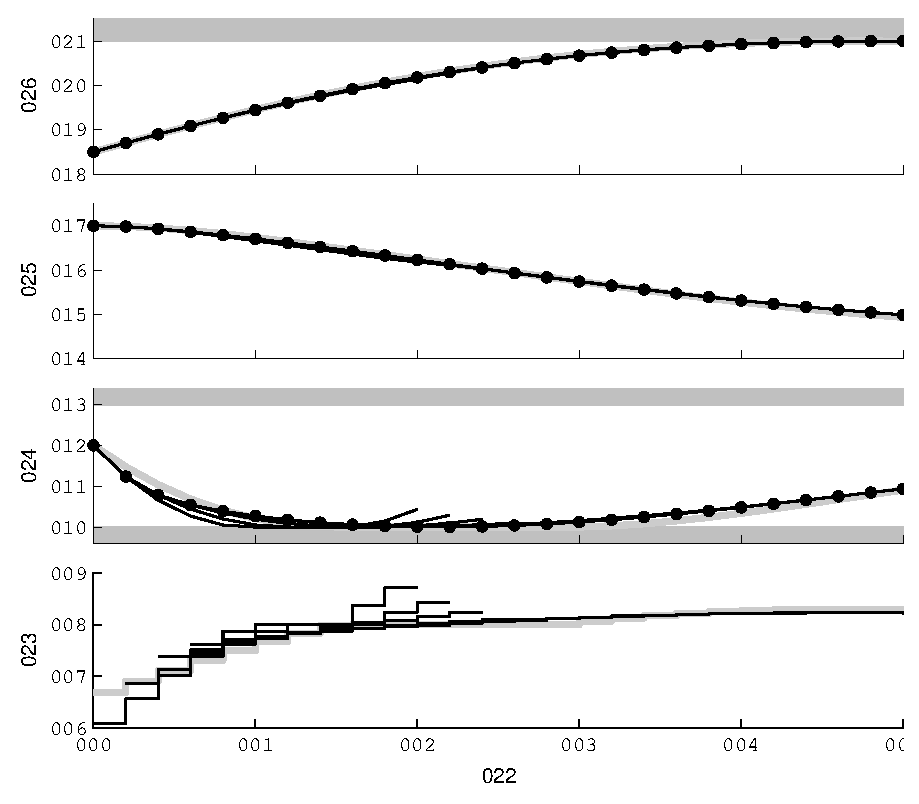
\includegraphics[width=.9 \linewidth,trim = 0cm 0cm 0cm 0cm]{3_MPC_Signals.eps}
    \caption[Trajektorienzeitverläufe der modellprädiktiven Regelkreise]{Zeitverläufe der Trajektorien der beiden modellprädiktiven Regelkreise; $T=\infty$ in Grau, $T=\unit[1.0]{s}$ in Schwarz; Ungleichungsnebenbedingungen repräsentiert durch graue Balken}
    \label{fig:MPC_Signals}
	\end{figure}
  




%\subsection{Parallelen zu Inevitable Collision States}
% - Keine Stabilitätsbetrachtung, sichert "`nur"' realisierbarkeit der Trajektorie
% - Keine Berücksichtigung weiterer NB?
% - Konstruktives Konzept? Eher nein, das ICS-Checker nicht gelöst

% Gütekritierium: If the cost is a kind of reward, as in investment planning or in most AI books, then maximization is preferred. [LaValle]
% Zur Seitenzahlreduktion: Nur Krümmungsregelung des Anhängers mit der Motivation, dass die überlagerte Optimierung erst noch behandelt wird, die der Mensch im Anhängerbeispiel übernimmt.

% Graicheninhalte:
% Lösen von Optimalsteuerungsproblem, Hinschreiben mit Tildegrößen oder so
% Prinzip MPC, Optimierung wird gelöst in jedem schritt

% \cite{allgower2004nonlinear}: 
% intuitive darstellung infinite horizont wie bei mir in der diss
% finiter horizont: endkosten müssen so ausgelegt werden, dass sie eine obere schranke für die ausstehenden kosten darstellen
% Unterscheidung zwischen nomineller stabilität und robustheit
%\cite{johansen2011introduction} wie allgower2004nonlinear, nur neuer

% Ideen
% Abprüfung der stabilität anhand von isolierten szenarien (z.B. isoliertes FAhrzeug)
% Echtzeitimplementierung in der Regelungstechnik versucht den Horizont so kurz zu halben wie möglich. Beim Fahrzeug auf Führungsebene ist das aber nicht möglich, da immer eine gewissen vorausschau erforderlich ist.
% Feasisbility / ics etc. ist nur sehr schwer zu berechnen / zeigen: deshalb heuristiken wie constant time gap control wichtig.
% modellidentifikation (wichtig sonst in der regelungstechnik) ist nicht wichtig auf führungsebene, wenn davon ausgegangen wird, dass krümmungen und beschleunigungen exakt umgesetzt werden.
% Dies ist auch der grund warum robustness auf führungsebene nicht so wichtig solange die unterlagerte regelung hinreichend gut ist. Kommentar bei robustheit hinzufügen, der auf robuste NMPC verweist, aber auch mit dem hinweis, dass robustheit hier mit unterlagerter regelung erreicht wird.



% Hier stabilisierung, auch durch überlagerte Optimierung
% Aus der Optimalität können stabilitätseigenschaften abgeleitet werden, weshalb im folgenden ein großer Wert auf optimierung gelegt wird.

% lavalle: 15.1.Lyapunov functions in planning
% Aber häufig keine Optimierung bis zum ziel möglich

% Bei stabilisierung: brockett1983asa zumindest erwähnen

%Dang übersicht über Einflussmöglichkeiten: Lenkung, Panzerbremse, Hinterradlenkung, torque vectoring
\newpage
\section{Robustheit\index{Robustheit} durch unterlagerte Regelungen}\label{sec:unterlagerteRegelung} \label{sec:sys_stab}
\zitat{Wennst den Baum siehst, in den du rein fährst, hast Untersteuern\index{Untersteuern}. \\ 
		Wennst ihn nur hörst, hast Übersteuern\index{Übersteuern}.}{Walter Röhrl}
%\subsection{Modellprädiktive Regelung im kaskadierten Regelkreis} 
Soll in die Manöverberechnung immer die neu erfasste Umfeldinformation einfließen, damit das Fahrerassistenzsystem schnell auf die Verkehrssituation reagiert, so hat die Trajektorienoptimierung permanent zu erfolgen. Entsprechend des vorhergehenden Abschnitts kann hierbei zusätzlich der aktuelle Systemzustand des Eigenfahrzeugs berücksichtigt werden. Gemäß Abschn.\,\ref{sec:stab_mpc} ist durch die entstehende Zustandsrückführung, zumindest theoretisch, eine vollständige Systemstabilisierung erzielbar. Die Analyse praktischer Anwendungen wie \cite{graichen_suboptimal, wahl2003ora, arnold2008mpt, schmidt2012hierarchischer} fördert jedoch zutage, dass der modellprädiktive Regelkreis in seiner reinen Form, bei der das optimierte Signal $\bs u(t)$ auch der tatsächlichen Streckenstellgröße entspricht (Steuerspannung, Bussignal etc.), nicht häufig zum Einsatz kommt. Stattdessen wird die Optimierung mit einer unterlagerten klassischen Regelung kombiniert. Die überlagerte modellprädiktive Regelung fungiert dann als sog.\ Führungsregler\index{Führungsregler}, dessen Ausgang dem unterlagerten Folgeregler als Referenz zugeführt wird und es entsteht eine Reglerkaskade\index{Kaskadenregelung}. Je nach Anzahl der unterlagerten Regelkreise generiert der Ausgang des unterlagerten Reglers die eigentliche Stellgröße oder wiederum das Referenzsignal für den nächsten unterlagerten Folgeregler\index{Folgereglung}. Auch das Elektronische Stabilitätsprogramm (ESP) (s.\ \zB \cite{handbuchFAS_Winner, liebemann2004safety, BHB2012_vanZanten_bremsanlage, vietinghoff2008nichtlineare, trachtler2005integrierte}) kann, ganz im Einklang mit dem modifizierten Drei-Ebenen-Modell in Abschn.\,\ref{sec:drei-ebenen-modell}, als unterlagerter Regler für den Fahrer als Trajektorienoptimierer angesehen werden, s.\ Abb.\,\ref{fig:ESP_Funktionsweise}.
%
\begin{figure}[h]
	\psfrag{U}[lc][lc][1.0]{Untersteuern\index{Untersteuern}}
	\psfrag{E}[lc][lc][1.0]{Übersteuern\index{Übersteuern}}
	\psfrag{B}[lc][lc][1.0]{Bremseingriff}
	\centering
  	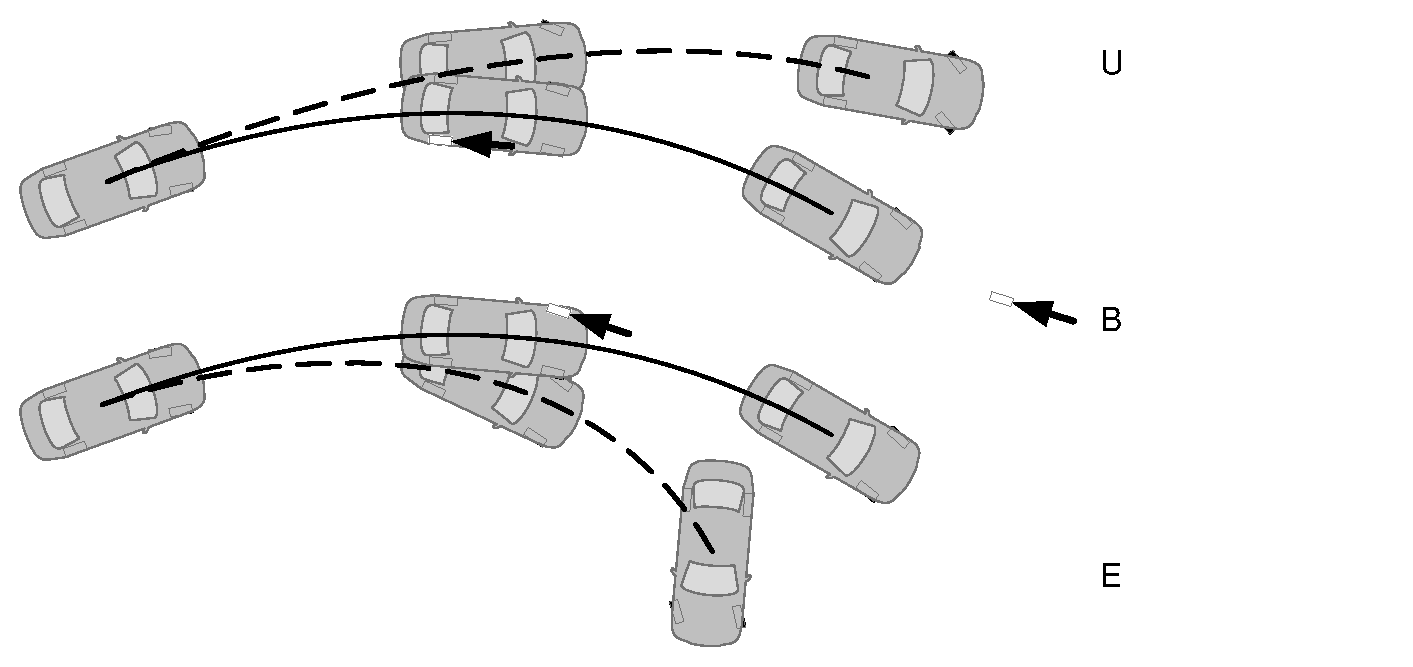
\includegraphics[width=1.05\textwidth,clip, trim = 0cm 0cm 0cm 0cm]{3_ESP_Funktionsweise.eps}
  	\caption[Funktionsweise vom ESP]{ESP sorgt dafür, dass sich das Fahrzeug auch in fahrphysikalischen Grenzsituationen sehr ähnlich zur gewohnten Dynamik der Normalfahrt verhält und damit der Mensch-Maschine-Regelkreis robust gegen Modellschwankungen und Störungen wird. Hierzu bremst das Fahrzeug einzelne Räder derart ab, dass sich das Fahrzeug möglichst ähnlich zu seinem linearen Einspurmodell verhält \cite{BHB2012_vanZanten_bremsanlage}.}
    \label{fig:ESP_Funktionsweise}
\end{figure} 


\subsection{Motivation unterlagerter Regelungen}
Aus der Praxis sind für die Kombination einer modellprädiktiven Regelung mit einer unterlagerten Folgeregelung folgende Hauptgründe zu nennen:

\textbf{Modellkomplexität:} \\
Die Wirkungsweise des klassischen Kaskadenregelkreises beruht darauf, dass der unterlagerte Regler eine Teilstreckendynamik stabilisiert und ihr zu Schnelligkeit verhilft, sodass sie im Entwurf des überlagerten Reglers vernachlässigt werden kann \cite{graf2003neue}. In gleicher Weise reduziert auch beim Entwurf der modellprädiktiven Regelung ein schneller unterlagerter Regler erheblich die Systemkomplexität des Prädiktionsmodells.

\textbf{Zykluszeiten und Übertragungslatenzen:} \\
Insbesondere die Überprüfung der Fahrtrajektorie auf Kollisionen mit dem Fahrzeugumfeld und die für bestimmte Optimierungsverfahren erforderliche numerische Simulation der Eigenfahrzeugdynamik beanspruchen einige Rechenzeit. %Dies verbietet bei vielen Optimierungsverfahren eine quasi-kontinuierliche\footnote{todo} Implementierung. 
Hinzu kommt, dass die Informationsübertragung zwischen Computer (das Steuergerät im Fall der Fahrerassistenz), Sensor und Aktor latenzbehaftet ist. Schnelle Streckendynamiken mit geringer Eigenstabilität werden damit nicht genügend rasch von der Optimierung beeinflusst. Ein unterlagerter Regler hingegen kann häufig direkt in der Aktorikelektronik integriert werden, wo ihm die Sensorinformation mit geringer Latenz zur Verfügung steht.

\textbf{Permanente Störungen und Modellfehler:} \\
Während impulsförmige Störungen bereits im nächsten Optimierungsschritt berücksichtigt werden können, leidet die Qualität des modellprädiktiven Regelkreises ganz erheblich unter permanenten Störungen und Modellfehlern\footnote{Beim Fahrzeug gehören dazu eine hängende Fahrbahn, Windeinflüsse, witterungsbedingte Reibwertänderungen und vor allem Vereinfachungen des komplexen Reifenkraftaufbaus.}. Da sich aufgrund der verschiedenartigen Einflussfaktoren eine genaue Störgrößenbeobachtung \cite{lunze2012regelungstechnik} bzw.\ Modelladaption \cite{kok95} oftmals sehr aufwändig gestaltet, stellt der Einsatz unterlagerter Regler eine häufig präferierte Alternative dar. Er sorgt dann dafür, dass sich die Dynamik der geregelten Teilstrecke trotz Störungen und Modellfehlern ähnlich dem Prädiktionsmodell verhält.

\textbf{Wiederverwendung unterlagerter Regelungen und Modularität:} \\
Die im Fahrzeug verbaute Aktorik (s.\ \abschn{sec:aktuatorik}) leistet bereits verlässlich ihren Dienst für verschiedene Stabilisierungssysteme wie ABS und ESP \cite{kiencke2005automotive, isermann2006frm}, s.\ Abb.\,\ref{fig:ESP_Funktionsweise}. Wie auch in anderen technischen Anwendungen wird hierbei vom Aktorhersteller bereits eine intensiv getestete und auf die jeweilige Hardware optimierte Regelung angeboten, die 1:1 in eine überlagerte modellprädiktive Regelung eingebettet werden kann. Neben der damit verbundenen Arbeitsersparnis wird, aufgrund der Einführung einer abstrahierten Schnittstelle, für den überlagerten Regelkreis eine weitgehende Unabhängigkeit von den Parametern der unterlagert stabilisierten Teilstrecke (Aktorik, Fahrzeugteildynamik etc.) erreicht. Die damit verbundene Steigerung von Flexibilität und Modularität ist in Anbetracht breiter Produktpaletten (Fahrzeugtypen und Sonderausstattungen) zur heutigen Zeit unverzichtbar \cite{rathgeber_ecc2014}.

%Angesichts der offensichtlichen Tragweite des Zusammenspiels von optimaler und klassischer Regelung für die Fahrerassistenz (bei gleichzeitigem Mangel an entsprechender Literatur) wird die Thematik in \abschn{sec:sys_stab} systematisiert und weiter vertieft.


% Robustheitsbetrachtungen sehr aufwändig. Als zweckmäßig haben sich aber unterlagerte regelungen herausgestellt, die die Fahrzeugbewegung umsetzen. Dann bleibt noch nichtlineare kinematik (Ebene Bewegung) übrig, die keine Parameterschwankungen unterliegt.
%\section{Systematische Betrachtungsweise der Stabilisierungsaufgabe} % oder so..

Da die Realisierung von unterlagerten modellprädiktiven Regelkreisen keinesfalls trivial ist, werden im Folgenden die möglichen Umsetzungsvarianten systematisiert. Hierbei sei vereinfachend angenommen, dass beim unterlagerten Regelkreis ein einzelner statischer, d.h.\ zustandsfreier, Regler eingesetzt wird. Eine Übertragung der Ergebnisse auf dynamische oder mehrfach-kaskadierte Regler ist jedoch ohne Einschränkung möglich.
Die Einteilung der kaskadierten Regelungsstruktur erfolgt nach dem asymptotischen Verhalten der unterlagerten Folgeregelungen.

\subsection{Nicht-asymptotische Folgeregelung} \label{sec:nichtasymptotischeFolgeregelung}
Aufgrund des Tiefpasscharakters der Aktorik ist in der Ein-Freiheitsgrad-Struktur, d.h.\ ohne Vorsteuerung, ein asymptotischer Folgeregler nicht realisierbar. Dennoch kann eine nicht-asymptotische Folgeregelung, insbesondere aufgrund der mit ihr verbundenen Einfachheit, in vielen Situationen einen wertvollen Beitrag liefern.
Die Integration des unterlagerten Folgereglers in den überlagerten modellprädiktiven Regelkreis ist denkbar einfach. Hierzu sei Abb.\,\ref{fig:KR_Unterlagerte_Stabilisierung} betrachtet, aus der unmittelbar ersichtlich wird, dass die überlagerte Optimierung (MPC) den durch die unterlagerte Rückführung $\bs x_1$ geschlossenen Regelkreis als neue Gesamtstreckendynamik $\Sigma'$ aufzufassen hat. Das Führungssignal des unterlagerten Folgereglers ist hierbei als neuer Systemeingang zu betrachten, und damit die Stellgröße $\tilde{\bs u}$ aus Optimalsteuersicht der MPC. \\
Bei geeigneter Auslegung der Folgeregelung weist das neue System $\Sigma'$ gegenüber der ursprünglichen Strecke $\Sigma$ ein gutmütigeres Verhalten auf, sodass der überlagerte modellprädiktive Regelkreis mit einer längeren Zykluszeit auskommt, da die Strecke während eines Optimierungszyklus durch die unterlagerte Stabilisierung nicht "`wegläuft"'. Darüber hinaus erleichtert die veränderte Streckendynamik die für bestimmte numerische Optimierungsverfahren erforderliche Simulation von $\Sigma'$, s.\ Abschn.\,\ref{sec:direkte_mehrfach_schiessverfahren}, oder sie weist durch die Rückführung so schnelle Teildynamiken auf, dass sie aus MPC-Sicht vernachlässigt werden können. \\
Falls keine Teildynamiken vernachlässigt werden können und die Rückkopplung im modellprädiktiven Regelkreis ohnehin häufig erfolgt, so kann der unterlagerten Regelung \iA keine robustheitssteigernde Wirkung in Bezug auf Modellfehler und Störungen zugeschrieben werden. Der Grund hierfür ist, dass es sich beim unterlagerten Regelkreis in der Rückkopplung um dasselbe $\bs x_1$ handelt wie in die modellprädiktive Regelung in $\bs x$ zurückgeführt wird. Anschaulich gesprochen invertiert damit die überlagerte Optimierung 1:1 die Folgeregelung im Modell $\Sigma'$, welche ja lediglich eine statische Abbildung von $\bs x_1$ und $\tilde{\bs u}$ auf $\bs u$ darstellt, sodass dort auch gleich $\bs u$ berechnet werden könnte.

\begin{figure}[h]
\centering
\newcommand{\smallsize}{.85}
		\psfrag{u}[cb][cb][1.]{$\bs u$}
		\psfrag{v}[cb][cb][1.]{$\tilde{\bs u}$}
		\psfrag{x}[cb][cb][1.]{$\bs x$}
		\psfrag{1}[cc][cc][1.]{$\Sigma$}
		\psfrag{m}[cb][cb][1.]{$\bs x_1$}
		\psfrag{g}[cb][cb][1.]{$\Sigma'$}
		\psfrag{c}[cc][cc][\smallsize]{\parbox[c]{7cm}{\begin{center}MPC\\ $\Sigma'$ \end{center}}}
				\psfrag{t}[cc][cc][\smallsize]{\parbox[c]{7cm}{\begin{center}Folge- \\ regelung \end{center}}}
	\includegraphics[width=.6\textwidth,clip, trim = 0cm 0cm 0cm 0cm]{2_KR_Unterlagerte_Stabilisierung.eps}
	\caption{Modellprädiktive Regelung mit unterlagerter Folgeregelung}
	\label{fig:KR_Unterlagerte_Stabilisierung}
\end{figure}

\subsection{Asymptotische Folgeregelung} \label{sec:asymptotische_folgeregelung}
Bevor nun die etwas aufwändigere Integration eines asymptotischen Folgereglers in den modellprädiktiven Regelkreis erläutert wird, soll als Vorstufe zunächst der Sonderfall betrachtet werden, in dem die Systemstellgröße $\bs u(t)$ aufgrund praktischer Anforderungen stetig verlaufen muss. Diese Herangehensweise ist erforderlich, wie im Beispiel der modellprädiktiven Abstandsregelung in Abschn.\,\ref{sec:mpc_acc}, wenn in der überlagerten Optimierung die Stellrate $\dot{\bs u}$ im Gütekriterium oder in den Nebenbedingungen (Stellratenbeschränkung) berücksichtigt werden muss. \\
Damit die Stetigkeitsbedingung an $\bs u$ erfüllt werden kann, muss in jedem Schritt die vorherige Stellgröße verfügbar sein, sodass die Aufgabe nur von einem dynamischen Regelkreis, der die vorherige Stellgröße als Zustand besitzt, erfüllt werden kann. Eine gleichermaßen einfache wie anschauliche Realisierung erfolgt entsprechend Abb.\,\ref{fig:KR_Integrator_Erweiterung} über die Systemerweiterung von $\Sigma$ um einen vorgelagerten Integrator, dessen Ausgang die Stellgröße $\bs u$ liefert. Gleichzeitig ist nun das Integral als Zustand $\bs z=\bs u$ des erweiterten Systems $\Sigma'$ aufzufassen und nebst $\bs x$ in die modellprädiktive Regelung zurückzuführen. Das dort zu lösende Optimalsteuerungsproblem hat nun das erweiterte System $\Sigma'$ zu berücksichtigen, da die Stellgröße $\tilde{\bs u}$ den Integratoreingang darstellt. Die Implementierung der Integratorerweiterung erfolgt durch numerische Integration von $\tilde{\bs u}(t)$.

\begin{figure}[h]
\centering
\newcommand{\smallsize}{.85}
	\psfrag{a}[cc][cc][\smallsize]{\parbox[c]{7cm}{\begin{center}MPC\\ $\Sigma'$ \end{center}}}
		\psfrag{i}[cc][cc][1.]{$\int$}
		\psfrag{u}[cb][cb][1.]{$\bs u$}
		\psfrag{v}[cb][cb][1.]{$\tilde{\bs u}$}
		\psfrag{z}[rb][rb][1.]{$\bs z\!=\!\bs u$}
		\psfrag{x}[cb][cb][1.]{$\bs x$}
		\psfrag{e}[br][br][1.]{$\Sigma'$}
		\psfrag{s}[cc][cc][1.]{$\Sigma$}
	\includegraphics[width=.6\textwidth,clip, trim = 0cm 0cm 0cm 0cm]{2_KR_Integrator_Erweiterung.eps}
	\caption{Modellprädiktive Regelung mit Integratorerweiterung}
	\label{fig:KR_Integrator_Erweiterung}
\end{figure}

Für die Unterlagerung der modellprädiktiven Regelung mit einer asymptotischen Folgeregelung ist ähnlich zu verfahren. Der Grund hierfür ist, dass von einer Folgeregelung nur realisierbare (insbesondere hinreichend oft stetig differenzierbare) Referenzverläufe asymptotisch stabilisiert werden können. \\
Da die asymptotische Folgeregelungsaufgabe keinesfalls die gesamte Systemdynamik umfassen muss, erfolgt im ersten Schritt entsprechend Abb.\,\ref{fig:KR_Unterlagerte_Folgeregelung} eine Unterteilung der Strecke in das asymptotisch zu stabilisierende Teilsystem $\Sigma_1$ und ihre restliche Dynamik $\Sigma_2$. Im zweiten Schritt wird der Regelkreis um das System $\tilde \Sigma_1$ erweitert, das so gewählt werden muss, dass dessen Ausgang dem Folgeregler nur realisierbare Referenzverläufe generiert. Darüber hinaus muss es ein ähnliches Streckenverhalten wie $\Sigma_1$ aufweisen, damit sich dessen Zustände $\tilde {\bs x}_1$ nicht allzu sehr von $\bs x_1$ unterscheiden, da nur erstere im Optimierungskriterium Berücksichtigung finden (s.\ Rückführung $\tilde {\bs x}_1$ in Abb.\,\ref{fig:KR_Unterlagerte_Folgeregelung}). \\
Aufgabe der Folgeregelung ist es nun, das System $\Sigma_1$hinreichend genau mittels $\bs u$ zu stabilisieren (im Idealfall asymptotisch), sodass $\tilde {\bs w}(t) \approx \bs w(t)$, also der Systemausgang von $\Sigma_1$ hinreichend genau dem von $\tilde\Sigma_1$ folgt. Der modellprädiktive Regelkreis kann dann nämlich auf Basis der Verkettung von simuliertem Teilsystem $\tilde \Sigma_1$ und Reststrecke $\Sigma_2$ entworfen werden, deren jeweilige Systemzustände $\tilde {\bs x}_1$ und $\bs x_2$ wiederum in das Optimalsteuerungsproblem rückzuführen sind. \\
Neben den zuvor erwähnten Vorteilen der nicht-asymptotischen Folgeregelung wird zusätzlich Robustheit gegen permanente Störungen und Modellfehler im Teilsystem $\Sigma_1$ erlangt. Allerdings wird sie mit einer erhöhten Anfälligkeit auf Impulsstörungen desselben Teilsystems erkauft.
Schließlich spiegeln sich diese nicht in den in die Optimierung rückgeführten Systemgrößen $\tilde {\bs x}_1$ wider, sondern müssen %nicht auf $\tilde\Sigma_1$ wirken und damit 
vom Folgeregler ausgeregelt werden.
%
\begin{figure}[h]
\centering
\newcommand{\smallsize}{.85}
			\psfrag{b}[cc][cc][\smallsize]{\parbox[c]{7cm}{\begin{center}MPC\\ $\tilde\Sigma_1 \Sigma_2$ \end{center}}}
		\psfrag{u}[cb][cb][1.]{$\bs u$}
		\psfrag{v}[cb][cb][1.]{$\tilde{\bs u}$}
		\psfrag{x}[cb][cb][1.]{$\bs x$}
		\psfrag{0}[cc][cc][1.]{$\tilde \Sigma_1$}
		\psfrag{r}[cc][cc][\smallsize]{\parbox[c]{7cm}{\begin{center}asympt.\ \\ Folgeregler  \end{center}}}
		\psfrag{1}[cc][cc][1.]{$\Sigma_1$}
		\psfrag{2}[cc][cc][1.]{$\Sigma_2$}
		\psfrag{w}[cb][cb][1.]{$\tilde{\bs w}$}
		\psfrag{n}[cb][cb][1.]{$\bs w$}
		\psfrag{m}[cb][cb][1.]{$\bs x_1$}
		\psfrag{k}[cb][cb][1.]{$\bs x_2$}
		\psfrag{l}[cb][cb][1.]{$\tilde {\bs x}_1$}
		\psfrag{f}[br][br][1.]{$\approx\!\bs 1$}
	\includegraphics[width=1\textwidth,clip, trim = 0cm 0cm 0cm 0cm]{2_KR_Unterlagerte_Folgeregelung.eps}
	\caption{Modellprädiktive Regelung mit asymptotischer Folgeregelung}
	\label{fig:KR_Unterlagerte_Folgeregelung}
\end{figure}

Beinhaltet nun das asymptotisch stabilisierte System die gesamte Streckendynamik $\Sigma$, sodass wie in Abb.\,\ref{fig:KR_Trajektorienplanung_Folgeregelung} dargestellt  $\Sigma_2$ verschwindet, entsteht ein sog.\ Führungsgrößengenerator\index{Führungsgrößengenerator} mit Modellfolgeregelung\index{Modellfolgeregelung} (vgl.\ auch \cite{roppenecker2009zustandsregelung}), was entsprechend Abschn.\,\ref{sec:begriff_tp} eine Trajektorienplanung mit unterlagerter Folgeregelung darstellt.
%wiederum große Ähnlichkeit mit der in Abb.\,\ref{fig:arbeitspunktwechsel_tp} vorgestellten klassischen Trajektorienplanung mit unterlagerter Folgeregelung aufweist.

\begin{figure}[h]
\centering
\newcommand{\smallsize}{.85}
			\psfrag{b}[cc][cc][\smallsize]{\parbox[c]{7cm}{\begin{center}MPC\\ $\tilde\Sigma$ \end{center}}}
		\psfrag{u}[cb][cb][1.]{$\bs u$}
		\psfrag{v}[cb][cb][1.]{$\tilde{\bs u}$}
		\psfrag{x}[cb][cb][1.]{$\bs x$}
		\psfrag{0}[cc][cc][1.]{$\tilde \Sigma$}
		\psfrag{r}[cc][cc][\smallsize]{\parbox[c]{7cm}{\begin{center}asympt.\ \\ Folgeregler \end{center}}}
		%\psfrag{1}[cc][cc][\smallsize]{\parbox[c]{7cm}{\begin{center}Teil- \\ system 1 \end{center}}}
		\psfrag{1}[cc][cc][1.]{$\Sigma$}
		%\psfrag{2}[cc][cc][\smallsize]{\parbox[c]{7cm}{\begin{center}Teil- \\ system 2 \end{center}}}
		\psfrag{w}[cb][cb][1.]{$\tilde {\bs w}$}
		\psfrag{n}[cb][cb][1.]{$w$}
		\psfrag{m}[cb][cb][1.]{$\bs x$}
		\psfrag{l}[cb][cb][1.]{$\tilde{\bs x}$}
	\includegraphics[width=.8\textwidth,clip, trim = 0cm 0cm 0cm 0cm]{2_KR_Trajektorienplanung_Folgeregelung.eps}
	\caption{Modellprädiktive Regelung mit nachgelagerter Folgeregelung}
	\label{fig:KR_Trajektorienplanung_Folgeregelung}
\end{figure}

Für die Implementierung der Systemerweiterung, also die weißen Kästen in Abb.\,\ref{fig:KR_Integrator_Erweiterung}-\ref{fig:KR_Trajektorienplanung_Folgeregelung}, bieten sich zwei grundsätzlich unterschiedliche Möglichkeiten an. Die erste besteht darin, die jeweiligen Differentialgleichungen mittels numerischer Standardverfahren in der Zykluszeit des Folgereglers zu lösen, also in Echtzeit zu simulieren, sodass letzterem in jedem Zeitschritt sein Referenzsignal zur Verfügung steht.
Die zweite Möglichkeit besteht darin, direkt die bei einigen Optimierungsverfahren intern als optimale Prädiktion $\bar{\bs x}^\ast(\tau)$ vorliegende Lösung heranzuziehen, s.\ Abb.\,\ref{fig:2_mpc_grundidee_u_x}. Es braucht im Anschluss des Optimierungsschritts die optimale Referenztrajektorie nur im relevanten Zeitabschnitt in der Zykluszeit des unterlagerten Reglers abgetastet und das Ergebnis zum richtigen Zeitpunkt dem Folgeregler weitergeleitet werden. Unbedingt zu beachten ist hierbei, dass nicht der Versuchung nachgegeben werden darf, anstelle von  $\tilde{\bs x}$ den gemessenen \bzw beobachteten Systemzustand $\bs x$ in die Optimierung zurückzuführen. Dann nämlich büßt das Gesamtsystem seine Robustheit gegen permanente Störungen und Modellfehler in der Weise ein, wie die fehlende Robustheit zuvor beim nicht-asymptotischen Folgeregler am Ende von Abschn.\,\ref{sec:nichtasymptotischeFolgeregelung} begründet wurde.

Zusammenfassend kann festgehalten werden, dass die Kombination aus modellprädiktivem Regelkreis und unterlagerter Folgeregelung große Vorteile in Bezug auf die Systemrobustheit bietet. 
Die Aufgabe der unterlagerten Folgeregelung ist hierbei, für ein gutmütigeres (Teil-) Streckenverhalten aus Sicht der überlagerten Optimierung zu sorgen, oder das stabilisierte System so zu beeinflussen, dass es trotz Störungen und Modellunsicherheiten dem Optimierungsmodell nahe kommt.
Hierbei entsteht aufgrund der variablen Größe des unterlagert stabilisierten Teilsystems ein Freiheitsgrad, der vom Entwicklungsingenieur so ausgenutzt werden muss, dass das Gesamtverhalten des modellprädiktiven Regelkreises ein ausgewogenes Verhältnis aus Robustheit gegen permanente Störungen bzw.\ Modellfehler und Gutmütigkeit bei Impulsstörungen aufweist. Eine generelle Empfehlung kann nicht ausgesprochen werden, da sich je nach umzusetzender Fahrerassistenzfunktion, eingesetzter Sensorik und Systemarchitektur die Anforderungen hinsichtlich Störunterdrückung, Genauigkeiten und Komfort stark unterscheiden. \\
% TODO: 
%
%Notiz: Neuplanung funkioniert bei manchen Planern nicht vom aktuellen Zustand, da dieser Stark diskretisiert ist und nur in kOmbination mit einem unterlagertn Regler funktioniert.
%
%\subsection{Praxisbeispiele}
%
% - Punktmassenmodell
% - Beispiele, die zur Motivation geführt haben, Stanford, CMU etc.
% - Exosystem
% - Führungsgröße muss für Folgeregelung hinreichend oft stetig diffbar sein (Lineare Strecke).
% - Simuliertes Modell kann vereinfacht sein (z.B. Punktmasse)
% - Sättigungsverhalten insbesondere bei Nichtlinearen Streckenteil auch interessant
%
% Werling diss: Leitet Impulsförmige Störungen auf Simuliertes System weiter, indem Zustände entsprechend gesetzt werden.
%
Zur Stabilisierung des \emph{gesamten} Fahrzustands existieren eine ganze Palette von praxiserprobten Regelungstypen, klassische \emph{PID} \cite{Muller-Bessler2006},  \emph{Sliding-mode-} \cite{eigel2010integrierte}, \citeltex{werling2014powerslide}, \emph{exakte ein-/ ausgangslinearisierende} \cite{Konig2007, atSonderheft08, soehnitz} \citeltex{werling2012trajektorienregelung}, \emph{robuste} \cite{walter_ecc2014, rathgeber_ecc2014} und \emph{optimierungsbasierte} Regler \cite{waldmann2009entwicklung, kessler2007konzept, weilkes2005zukunftige}, um nur einige zu nennen. Allesamt sind grundsätzlich dazu geeignet, auch einen reduzierten Fahrzustandsvektor zu stabilisieren. Letztendlich kann aber nur die konkrete Kombination aus MPC-Regelkreis und unterlagertem Regler auf Robustheit beurteilt werden.

%Hierbei kommen alle modernen Regelungsverfahren wie Sliding-mode \cite{eigel2010integrierte}, Exakte Ein-/Ausgangslineareisierung \cite{Konig2007, atSonderheft08} \citeltex{werling2012trajektorienregelung}, \citeltex{werling2014powerslide}
%robuste Verfahren  unterschiedliche Längs-Quer-Kopplungseffekte \cite{eigel2010integrierte} berücksichtigen. 
%\cite{waldmann2009entwicklung}  %mittels LQR-tracker

%\cite{minoiu2009driver} % Heading-control mit LMIs
%\cite{kessler2007konzept} % Lineare MPC zur Querführung für Nutzfahrzeuge -> s. auch Kap 6 Riccati
%\cite{soehnitz} % E/A-Linearisierung

% Driftregler:
% Sliding-mode: wird auch für die Querregelung eingesetzt: 
%\cite{eigel2010integrierte}
% Bestimmung des Positionsregelfehlers beim Positionstracking, zwischen den Planungszeiten.
% --macht ganzheitliche Implementierung einfacher

%\cite{Muller-Bessler2006}
%\cite{weilkes2005zukunftige} % altes Bosch paper zur Quer- und Längsführung, Kopplung in ihrem sinne

%\cite{Bender2007} 					% EP, sigmoide von proreta, keine Optimierung, parameter ergeben sich aus randbedingungen
%\cite{keller2011active} 		% EP, Polynome, keine Optimierung

 
%Zusammenfassend kann bemerkt werden, dass die großen Vorteil der ortsfesten Koordinaten für die Manöverplanung, die Positionsregelung oder das Objekt-Tracking/lokale Kartieren darin bestehen, dass die \textbf{Kopplenavigation}
%\begin{itemize}
	%\item aufgrund der Integration der Fahrzeugbewegung keinerlei Positions- und Ausrichtungssprünge aufweist (s.\ z.B.\ stanfordsmoothcoordinates),
	%\item eine nahezu permanente Verfügbarkeit aufweist und
	%\item bei Einsatz von Inertialsensorik mit einer kurze Zykluszeit (z.B.\ $\unit[10]{ms}$) verfübar ist.
%\end{itemize}
%Eine \textbf{globale Eigenlokalisierung} hingegen ist nach aktuellem Technikstand durch
%\begin{itemize}
	%\item Korrektursprünge gekennzeichnet, etwa am Tunnelende, an dem wieder ein GPS-Signal plötzlich verfügbar ist, oder bei in Sicht kommenden markanten Landmarken und
	%\item eine geringe Verfügbarkeit insbesondere innerhalb der Stadt gekennzeichnet,
%\end{itemize}
%sodass von ihr nur die Komponenten abhängen sein sollten, welche auf eine absolute Referenz angewiesen sind.
%



%Solange dessen Position, etwa von einer Kamera geliefert, in den Fahrzeugfesten Koordinaten verfügbar ist, muss sie mittels der von der Koppelnavigation gelieferten Koordinatentransformation in die Ortsfesten (wenn auch driftbehafteten) Koordinaten umgerechnet werden, wo ebenfalls das Notmanöver geplant wird. Verliert die Fahrzeugsensorik das Hindernis während des Ausweichens, so beläuft sich der Abstandsfehler zum Hindernis während des Ausweichens auf wenige Zentimeter.


%Überleitung zu smooth coordinates: trotz GPS eingesetzt weil so robust.




%Kartesische Koordinaten zu homogene Koordinaten: $[x,y]^\T \rightarrow [x,y,1]^\T$
%Translation
%\begin{align*}
	%\left[\begin{array}{c} x' \\ y' \\ 1 \end{array}\right] = \left[\begin{array}{ccc} 1 & 0 & t_x \\ 0 & 1 & t_y \\ 0 & 0 & 1 \end{array}\right] \cdot 
	%\left[\begin{array}{c} x \\ y \\ 1 \end{array}\right]
%\end{align*}
%
%Rotation
%\begin{align*}
	%\left[\begin{array}{c} x' \\ y' \\ 1 \end{array}\right] = \left[\begin{array}{ccc} \cos \alpha & -\sin\alpha & 0 \\ \sin\alpha & \cos\alpha & 0 \\ 0 & 0 & 1 \end{array}\right] \cdot 
	%\left[\begin{array}{c} x \\ y \\ 1 \end{array}\right]
%\end{align*}

% Langsame fahrt: beta_ha = 0 -> beispiel
% Triangulation
% Eine Absolute Positionierung kann sogar schädlich sein, dann wenn die Eigenlokalisierung springt, was für viele Algorithmen und Funktionen viel schlimmer ist als eine kleine durchgängige ungenauigkeit (drift)
% Erfolgt eine 1x Planung des Einparkmanövers, so muss während der Einregelung des Einparkvorgangs ebenfalls die aktuelle Position relative zur anfänglichen Position bestimmt werden, an der die Einparkkurve berechnet wurde.
% Überleitung zu Koppelnavigation: Zur Berechnung der Relativposition zu einer in der Vergangenheit liegenden Position kann die Fahrzeugbewegung aufintegriert werden und es wird von Koppelnavigation (engl. dead reckoning) gesprochen. Häufig wird Odmomentrie synonym verwendet, was aber nicht ganz korrekt ist, da streng genommen nicht nur die Räder herangezogen werden.
% Drift erklären, ist aber nicht schlimm, da nach der differenzbildung der absolutfehler sich nur auf das kleine Zeitintervall auswirkt
% Lenkradwinkel nicht vergessen bei ganz kleinen Geschwindigkeiten, da Gierratensensor dann relativ stärker driftet
% Das Ergebnis der Koppelnavigation kann zur Eigenlokalisierung verwendet werden, s. später.
% Eingangsgrößen für die Eigenlokalisierung eines Körperfesten Referenzpunkts: Bewegungsrichtung und Geschwindigkeit des Körpers im Referenzpunkt
%Zur Bestimmung der Gierbewegung eignet sich die ESP-Gierratensoensorik (hohe GEschwindigkeit) oder die Auswertung der Fahrzeugdynamik unter Berücksichtigung des aktuellen Lenkwinkels
% Insgesamt ergibt sich dann die Bewegungsdynamik zu
%\begin{align*}
	%\dot x_1 &= v \cos(\psi + \beta) \\
	%\dot x_2 &= v \sin(\psi + \beta) \\
	%\dot   \psi &= r
%\end{align*}
% Beispielbild: Drift mit großem Absolutfehler aber kleinem Relativfehler
		% Erklärung warum häufig Drift in der Loklisierung nicht schlimm ist
% Implementierung: Koppelposition wird als "korrekt" betrachtet, Ursprung kann innerhalb numerischer Genauigkeiten beliebig gewählt werden, da er sich bei der Differenzbildung aufhebt. Vorteil: Position springt nicht. Für die Verwendung absoluter Karteninformation (Straßenkarten) ist noch eine absolute Eigenlokalisierung erforderlich. Diese dient ausschließlich dazu absolute Landmarken (Straßen) in die Koppelposition zu transformieren. Zitat Stanford (smooth coordinates)
% Ich tue einfach so also ob die Koppelposition meine tatsächliche Fahrzeugposition ist und merke mir von Hindernissen etc. die Position in den lokalen Koordinaten. Habe ich das Hindernis erst kürzlich gesehen, so kann ich mir sicher sein, ...
% Wichtig auch für die Umfeldwahrnehmung und Szeneninterpretation


% ------------------------


% Falls Trajektorien für alle Zustände geplant wird, dann eignet sich Riccati zur Stabilisierung. Häufig wird aber nur für Brunowsky-Zustände geplant, dann stab durch E/A-Lin

%\label{sec:projektion} % noch unterbringen!

% Aufbau: 
% 2. Kap. Modellprädiktive Regelung im kaskadierten Regelkreis (ca. 5 Seiten) hier her kopieren, da schon sehr speziell und Kapitel sonst zu lang.
% Regelungssysteme von ABS über ESP hin zu Positionsregelung (von Stabilisierungsebene Richtung Führungsebene, Weg wird aufgezeigt, Motiviert auch, warum Hill-Climb control zb. nicht ausführlich behandelt wird, wohl aber ESP und ABS).


%\begin{figure}[h]
	%\psfrag{k}[cb][cb][1.0]{$v$}
	%\psfrag{l}[cb][cb][1.0]{$v_\text{ref}$}
	%\psfrag{m}[cb][cb][1.0]{$\lambda_1$}
	%\psfrag{n}[cb][cb][1.0]{$v_\text{Rad}$}
	%\psfrag{G}[cc][cc][1.0]{Geschwindigkeiten}
	%\psfrag{R}[cc][cc][1.0]{Radbeschleunigung}
	%\psfrag{B}[cc][cc][1.0]{Bremsdruck}
	%\psfrag{A}[cr][cr][1.0]{$A$}
	%\psfrag{b}[cr][cr][1.0]{$a$}
	%\psfrag{c}[cr][cr][1.0]{$-a$}
	%\psfrag{t}[cr][cr][1.0]{$t$}
	%\psfrag{0}[ct][ct][1.0]{Phase $0$}
	%\psfrag{1}[ct][ct][1.0]{$1$}
	%\psfrag{2}[ct][ct][1.0]{$2$}
	%\psfrag{3}[ct][ct][1.0]{$3$}
	%\psfrag{4}[ct][ct][1.0]{$4$}
	%\psfrag{5}[ct][ct][1.0]{$5$}
	%\psfrag{6}[ct][ct][1.0]{$6$}
	%\psfrag{7}[ct][ct][1.0]{$7$}
	%%\psfrag{M}[cc][cc][1.0]{Radbeschleunigung}
%\centering
%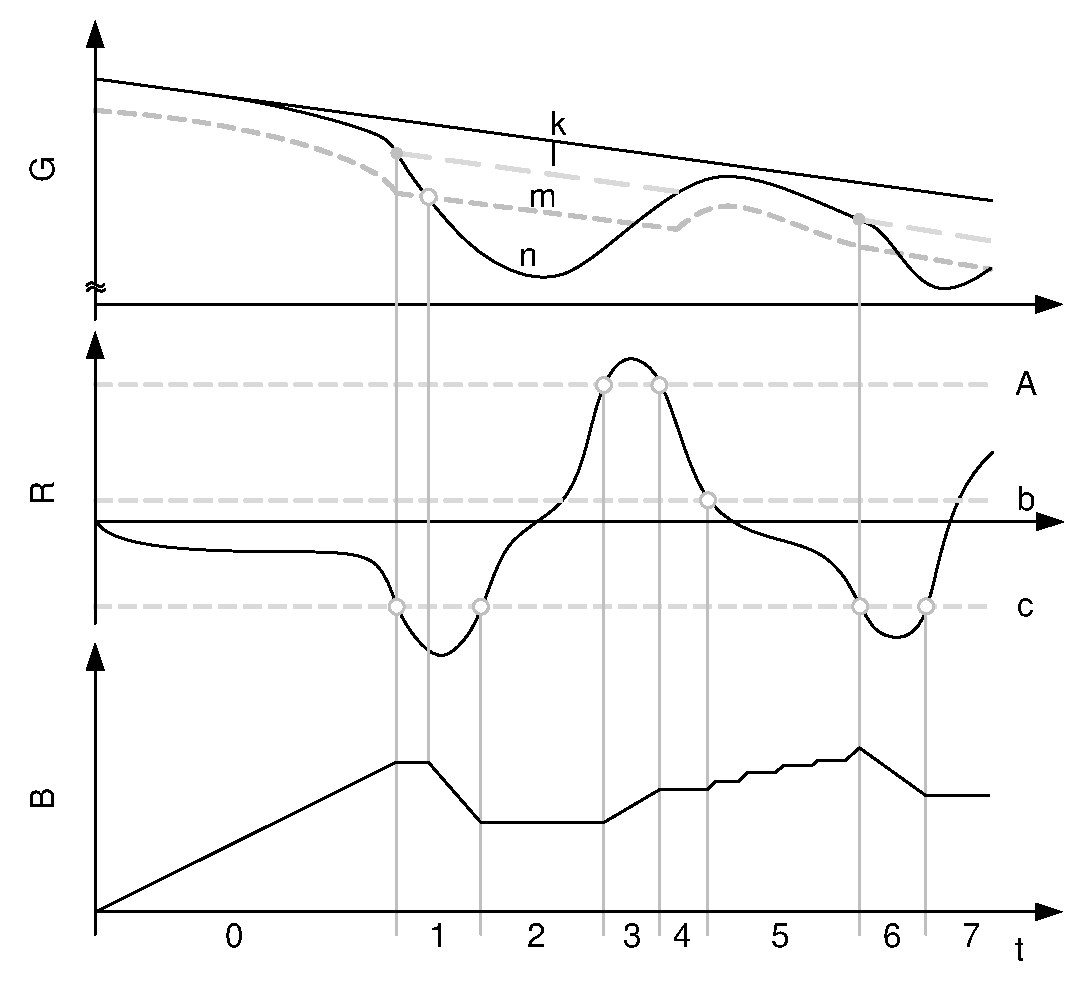
\includegraphics[width=1.0\textwidth,clip, trim = 0cm 0cm 0cm 0cm]{3_ABS_Signale.eps}
 %\caption{TODO}
 %\label{fig:abs_signale}
%\end{figure} 

% EPS Funktionen: 
% Geradeauslauf Korrektur, 
% Lane departure Warning/ support
% Fahrdynamische Lenkmomentenepfehlung (mu-split)
% Parklenkassistent


% Beispiel Seitenwindkompensation: Störbeobachter

% Überaktuiertes System -> Unterlagerte Regelung übernimmt Bremsverteilung, wird nicht in der Planung berücksichtigt
% Virtuelle Deichsel -> Heuristik
% Stanley -> Ebenfalls Heuristik -> Verallgemeinerung: E/A-Linearisierung
% ABS, ESP (Verdeutlicht am Doppelspurwechsel)

% Impedanzregelung ganz wichtig, da ja bei der Teilautomatisierung der FAhrer eine bedeutende Rolle spielt.

%[Regelung, Projektion, Invariante Fehlerdynamik]
%	\section{Systemmodellierung}
	%	\subsection{Fahrzeug} \label{sec:fahrzeugmodellierung}
	%	\subsection{Reifen} \label{sec:reifenmodellierung}
	%	\label{sec:lenkkinematik} % todo
	%	\label{sec:lenkdynamik} % todo
	%	\cite{dang2012steering} % Lenken ist viel schneller als Einzelradbremsung etc.


%\subsection{Aktorik}
%\cite{eigel2010integrierte} % Behandelt unterschiedliche Stellgrößen in der Lenkung
%\subsection{Längs- und querdynamische Kopplungseffekte}
 % und Literatur darin
% 1) Kopplung durch Geschwindigkeit (trivial)
% 2) Kopplung durch Kinematik (beim Positionstracking)
% 3) Kopplung an Reifen, dynamische Radlasten etc., Kurvenwiederstand
		
%		\subsection{Elektronisches Stabilitätsprogramm (ESP)} \label{sec:ESP}
		%\cite{BHB2012_vanZanten_bremsanlage} % Vorlage!
		%\cite{liebemann2004safety} % BOSCH ESP
		% ASR: Antrieb
		% Bremsassistent
		% Hill Hold Control
		
		% ESP muss keinen Fahrerwunsch schätzen, da durch übergeordnete Ebene Sollmanöver bekannt ist

%		\subsection{Aktiv- und Hinterachslenkung}
%		\subsection{Torque Vectoring} \label{sec:torque_vectoring}
		% \emph{torque vectoring} \cite{piyabongkarn2007use, fallah2012controller}
		% mu-split!
%[ABS, DSC]
% Seitenwindassistenz (Automatische Störgrößenkompensation, Daimler etc.)
%	\section{Fahrzeuglängsregelung}
%		\subsection{Adaptive Cruise Control (ACC)} \label{sec:acc}
%		\subsection{Notbremssysteme}
%		\label{sec:Hinterachslenkung} % todo unterbringen
%	\section{Pfadstabilisierung}
	%Fahrzeug Regelung: Literatur aus paper von Daniel Hess, IV 2013
	%\cite{atSonderheft08} %E/A-Linearisierung für Querregelung
%	\label{sec:einparksystem} %todo
% Kinematische Querregelung: ähnlichkeit mit
%\cite{Werling2010a}
%		\subsection{Projektion zur Fehlerbestimmung}
		% Abstandsbestimmung mit gradientenabstieg (s. Diss Anhang) -> Verweis auf Kap. Statische Optimierung!
%		\subsection{kinematisches Einspurmodell}
%		\section{Eingriffsstrategien}
%\begin{figure}[h]
	%\psfrag{d}[cc][c][1.0]{$\delta$}
	%\psfrag{M}[cb][cb][1.0]{$MP$}
	%\psfrag{v}[cr][cr][1.0]{$v$}
	%\psfrag{p}[cc][cc][1.0]{$\psi$}
	%\psfrag{l}[cr][cr][1.0]{$l$}
	%\psfrag{x}[cl][cl][1.0]{$[x_1, x_2]$}
%\centering
%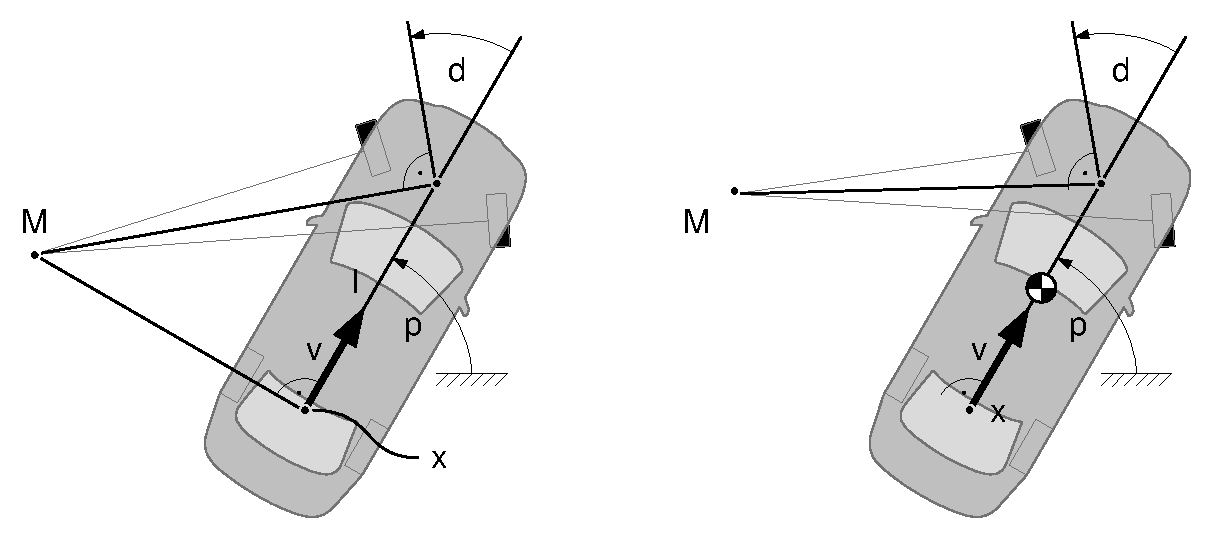
\includegraphics[width=1\textwidth,clip, trim = 0cm 0cm 0cm 0cm]{3_Einspurmodelle.eps}
 %\caption{Einspurmodell}
 %\label{fig:todo}
%\end{figure} 
		%\subsection{nichtlineares Einspurmodell}
	%\section{Trajektorienstabilisierung}
		%\subsection{Invariante Fehlerdynamik}
		%\subsection{Positionstracking}

\section{Neuer Algorithmus zur Gespannstabilisierung\index{Gespannstabilisierung}} \label{sec:anhaenger}
Während für die Vorwärtsfahrt die sog.\ \emph{aktive Gespannstabilisierung} (\emph{trailer stability assist}) \cite{BHB2012_vanZanten_bremsanlage}, \iA als Teil von ESP, das Schlingern eines Anhängers verhindert, ist der Fahrer beim rückwärtigen Rangieren auf sich alleine gestellt.
%
	%  zu erwähnen: Trailer Stability Assist (TSA)
		% Riccati zum einstellen von e/A-Z Stab Parameter
%\subsection{Hintergrund}
% Während mit dem Zugfahrzeug beim Vorwärtsfahren lediglich ein zusätzlicher Sicherheitsabstand zu kurveninneren Hindernissen eingehalten werden muss, um das Kurvenschneiden des Anhängers zu kompensieren, empfinden viele Fahrer die zum Zurücksetzen des Anhängers erforderlichen Lenkbewegungen als nicht intuitiv. 
Als nicht intuitiv wird hierbei die %nicht-holonome
Gespanndynamik empfunden, welche beim Rückwärtsfahren zur Kursänderung ein kurzzeitiges Lenken entgegen der Wunschrichtung erfordert. %Wird diese Lenktechnik nicht beherrscht, droht -- neben der Beschädigung von Fahrzeug und Anhänger -- dem Gespannführer ein nervenaufreibendes Unterfangen im öffentlichen Straßenverkehr. Hier kann eine automatische Stabilisierung des Anhängers für Entlastung des Fahrers sorgen.
Im Folgenden wird daher ein neues Stabilisierungsverfahren \citeltex{werling2014anhaenger,Werling2014trailer} für die Gierbewegung eines Anhängers vorgestellt, das den Fahrer als überlagerten Regler begreift, den es gilt, bestmöglich durch aktive Lenkeingriffe eines unterlagerten Reglers zu unterstützen. 

%Aus Kostengründen muss im Pkw-Bereich auf eine aktuierte Anhängerkupplung \cite{hoffmann2007gespannmanagement} verzichtet werden. Hierdurch steht lediglich die Lenkung zur gezielten Beeinflussung des Gespanns zur Verfügung.
Dank der interessanten nichtlinearen Struktur der Gespanndynamik existiert in der Literatur eine Vielzahl von Ansätzen, welche die Bewegung des Fahrzeuggespanns entlang vorgegebener Pfade und Trajektorien stabilisieren. Aufgrund der hohen Modellgüte sowie der einfach zu bestimmenden geometrischen Fahrzeug- und Anhängerparameter eignen sich insbesondere exakt ein-/\-ausgangs-\index{Exakte Ein-/\-ausgangslinearisierung} \bzw zustandslinearisierende\index{Zustandslinearisierung} Regelungsansätze \cite{allgower1993nichtlinearer, rothfuss1997fnz}, die auf der Kompensation der Systemnichtlinearitäten durch Zustandsrückführungen basieren. Die Herangehensweise wird auch hier verfolgt. Viele Arbeiten beschränken sich allerdings auf den Fall, bei dem der Kupplungspunkt mit dem Achsmittelpunkt des Zugfahrzeugs zusammenfällt (\emph{standard one-trailer-system}) \cite{tilbury1992steering, rouchon1993flatness2, sampei1995arbitrary}, wodurch die Mittel\-punkts\-koor\-di\-na\-ten der Anhängerachse einen flachen Ausgang (s.\ Abschn.\,\ref{sec:flachheitbasierte_para}) des Gespanns darstellen \cite{rouchon1993flatness1}. Diese Vereinfachung ist beim Pkw nicht zulässig, da der Kupplungspunktversatz %kingpin hitch, off-axle hitchching
in der Größenordnung der Länge der Anhängerdeichsel liegt \cite{altafini2001some}. \\
In \cite{rouchon1993flatness1} wird daher auch für den allgemeinen Fall (\emph{general one-trailer-system}) die Flachheit nachgewiesen. Während die Eigenschaft für eine Bahnplanung von höchstem Interesse ist (s. dazu den Ausblick in Abschn.\,\ref{sec:eval_trailer}), verzichtet der hier vorgestellte Ansatz bewusst auf die Stabilisierung eines flachen Ausgangs. Grund hierfür ist die dadurch erzielbare Reduktion der zu stabilisierenden Systemzustände, was durch die %damit verbundene 
gutmütige interne Systemdynamik des Gespanns (s.\ Abschn.\,\ref{sec:nulldynamik}) ermöglicht wird, vgl.\ \cite{Werling2010a}. \\ % Übernahme der Zeittrafo
Alternative Stabilisierungsmethoden, die den Kupplungsversatz berücksichtigen, werden in
\cite{pradalier2008robust,  % in der Praxis ist die Lenkratensättigung kein Problem, solange die Dynamik hinreichend modelliert wird, s. PT1-Modell, Kaskadiert, Kein asympt. Fehlerverhalten, schlechte Ergebnisse
schwarz2009generisches, % Kein Asymptotisches Fehlerverhalten 
gonzalez2009backing} % Kaskadiert, kein asymptotisches Tracking (s. Ergebnisse).
vorgestellt. Die dort beschriebenen Rückführungsgesetze basieren auf einer Kaskade von Querregelung und unterlagerter Knickwinkelstabilisierung. Dabei wird allerdings die Dynamik letzterer vernachlässigt, sodass die Regelung kein asymptotisches Fehlerverhalten aufweist. \\
%Der erste Teil des Beitrags greift die Idee dieser Knickwinkelstabilisierung jedoch auf, welche grundsätzlich dazu geeignet ist, dem Fahrer beim Rückwärtsfahren mit Anhänger als eigenständiges System zu assistieren. 
Die Vorteil des nachfolgend hergeleiteten Stabilisierungsgesetzes besteht darin, anstelle der Festwertregelung des Knickwinkels eine \emph{asymptotische Folgeregelung} für die \emph{Fahrkrümmung} des Anhängers zu entwerfen. Hierdurch ist es für den Fahrer möglich, etwa über einen Drehknopf, den Anhänger nahezu verzögerungsfrei zu lenken, ähnlich einem ferngesteuerten Auto. \\
%Der zweite Teil des Beitrags fokussiert auf die Pfadstabilisierung. Der hier vorgeschlagene Ansatz weist keine kaskadierte Struktur auf, sondern wird entsprechend der Vorgehensweise der exakten Ein-/Aus\-gangs\-linearisierung "`am Stück"' entworfen. Er sichert dadurch eine asymptotische Fehlerdynamik, deren Eigenwerte anhand weniger Parameter gezielt auf das Sensorrauschen abgestimmt werden können.
%im öffentlichen Straßenverkehr auch der Gesichtsverlust.

%Der Beitrag gliedert sich wie folgt. In Abschn.\,\ref{sec:anhaengerdynamik} wird zunächst das verwendete Gespannmodell vorgestellt, welches den beiden anschließenden ein-/aus\-gangs\-li\-ne\-arisier\-end\-en Reglerentwürfen zugrunde liegt.\\
%Das Modell wird in Abschn.\,\ref{sec:kruemmungsstab} einer Zeit\-trans\-for\-ma\-tion unterzogen, die der Singularitätsvermeidung im Stand dient.
%%bei den  Reglerentwürfen . 
%Der anschließende Reglerentwurf zielt auf das assistierte Zurücksetzen ab, indem der fahrergegebene Krümmungsverlauf stabilisiert wird. Wichtig hierbei ist die Vermeidung irreversibel großer Knickwinkel zwischen Fahrzeug und Anhänger sowie der Stellgrößensättigung der Lenkung. Daher wird die Nulldynamik des Systems auf Stabilität untersucht, um da\-raus Anforderungen an den Sollkrümmungsverlauf herzuleiten, welche durch die Einführung einer dynamischen Sättigungsfunktion zwischen Fahrer und Regler sicher erfüllt werden. \\
%Abschn.\,\ref{sec:pfadstab} widmet sich der Pfadstabilisierung, die zunächst eine Systemerweiterung des Gespanns um dessen zeittransformierte Pfadfolgedynamik erfordert. Im Anschluss erfolgt der zugehörige Reglerentwurf, wobei auf Ergebnisse des vorangegangen Abschnitts zurückgegriffen wird. \\
%Die Evaluation der vorgestellten Regelungskonzepte erfolgt schließlich in Abschn.\,\ref{sec:eval_trailer} anhand realer Fahrversuche mit einem Pkw-Gespann. 


\subsection{Nichtlineare Anhängerdynamik} \label{sec:anhaengerdynamik}
Da Anhänger grundsätzlich nur mit niedrigen Querbeschleunigungen zurückgesetzt werden, können die sog.\ Schräglaufwinkel an den Reifen des Gespanns vernachlässigt werden. Wie Abb.\,\ref{fig:KESM_Gespann} verdeutlicht, definieren hierdurch die Reifenausrichtungen über die Momentanpole $\mathrm{MP}_v$ und $\mathrm{MP}_t$ die Kinematik von Fahrzeug und Anhänger. Mit der Fahrzeugausrichtung $\psi_v$ und der Hinterachsgeschwindigkeit $v_v<0$ sowie mit dem effektiven Lenkwinkel $\delta$ der Vorderräder und dem Achsabstand $l_v>0$ ergibt sich die Fahrzeuggierdynamik (vgl.\ \zB \cite{atSonderheft08}) zu
%$l_v$ Hypotenuse
\begin{align}
	\dot \psi_v & = v_v \frac{\tan\delta}{l_v} \label{eq:fzgmodell:psi_v_dot}.
\end{align}
Entsprechend der Herleitung in \ref{app:herleitung_anhaengerdynamik} wird die Anhängergierdynamik durch
\begin{align}
\negspace	 
	\dot\psi_t &= \frac{v_v}{l_t} \left[\sin\left(\psi_v \! - \! \psi_t\right) - l_c\cos\left(\psi_v  \! - \!\psi_t\right) \frac{\tan\delta}{l_v} \right]  \label{eq:fzgmodell:psi_t_dot}
\end{align}
mit der vorzeichenbehafteten Anhängergeschwindigkeit 
\begin{align}
\negspace
	v_t &:= v_v \left[ \cos\left(\psi_v  \! - \! \psi_t\right) + l_c\sin\left(\psi_v  \! - \! \psi_t\right) \frac{\tan\delta}{l_v} \right] \label{eq:fzgmodell:v_t}
\end{align}
beschrieben. %An dieser Stelle sei angemerkt, dass die Betrachtung der Fahrzeuggeschwindigkeit $v_v<0$ als zeitabhängiger Systemparameter sowohl die Kombination mit einer manuellen (s.\ später Abschn.\,\ref{sec:eval_trailer}) als auch mit einer separaten automatischen Antriebsregelung ermöglicht. Dadurch ist die Lenkung als alleiniger Systemeingang anzusehen. 
Zur Vermeidung von Überschwingen ist das Verzögerungsverhalten der Lenkaktorik unbedingt zu modellieren und im Entwurf zu berücksichtigen. In der Praxis hat sich aufgrund der schnellen Dynamik der unterlagert eingesetzten Moment- und Drehratenregelung die Modellierung des Lenkwinkelübertragungsverhaltens %r Winkelpositionsregelung 
der Aktorik als PT$_1$-Glied
\begin{align}
	\dot\delta &= \frac{1}{T}\left[u-\delta\right] \label{eq:assistiert:delta_dot}
\end{align}
bewährt \cite{pradalier2008robust}. Hierbei beschreibt $T>0$ die Zeitkonstante und $u$ die dem Lenkaktor übermittelte Sollvorgabe -- und damit die Stellgröße des Systems. % hab: Kleinsignalverhalten!

\begin{figure}
    \psfrag{MPv}[lb][lb][1.0]{$\mathrm{MP}_v$}
	\psfrag{MPt}[lc][lc][1.0]{$\mathrm{MP}_t$}
	\psfrag{delta}[cc][cc][1.0]{$\delta$}
	\psfrag{rv}[lt][lt][1.0]{$\boldsymbol r_v$}
	\psfrag{rt}[rb][rb][1.0]{$\boldsymbol r_t$}
	\psfrag{rc}[cc][cc][1.0]{$\boldsymbol r_c$}
	\psfrag{vv}[rb][rb][1.0]{$\boldsymbol v_v$}
	\psfrag{vt}[lt][tl][1.0]{$\,\boldsymbol v_t$}
	\psfrag{vh}[lc][lc][1.0]{$\boldsymbol v_c$}
	\psfrag{psiv}[tr][tr][1.0]{$\psi_v$}
	\psfrag{psit}[rt][rt][1.0]{$\psi_t$}
	\psfrag{dpsi}[lb][lb][1.0]{$\,\Delta\psi$}
	\psfrag{lt}[rb][rb][1.0]{$l_t$}	
	\psfrag{lv}[rb][rb][1.0]{$l_v$}	
	\psfrag{lc}[rb][rb][1.0]{$l_c$}	
    \centering
    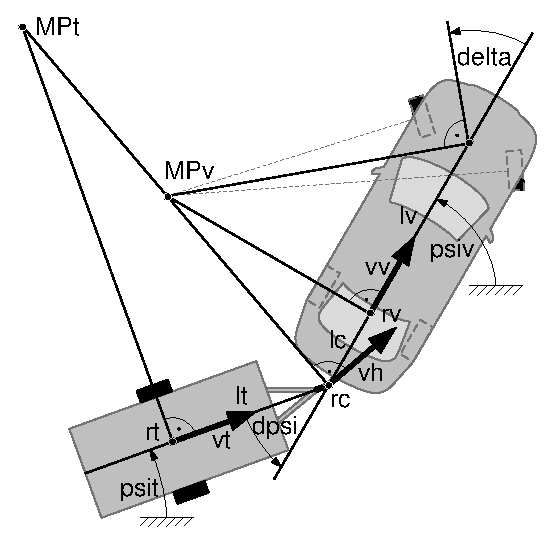
\includegraphics[width=.6 \linewidth,trim = 0cm 0cm 0cm 0cm]{3_KESM_Gespann.eps}
    \caption[Kinematisches Einspurmodell des Fahrzeuggespanns]{Kinematisches Einspurmodell des Fahrzeuggespanns \citeltex{werling2014anhaenger}}
    \label{fig:KESM_Gespann}
\end{figure}



%\subsection{Gierdynamikstabilisierung des Anhängers} \label{sec:kruemmungsstab}
\subsection{Zeittransformation} \label{sec:zeittrafo}
%Da im Stand zur Stabilisierung mittels glatter Rückführung das notwendige Brockett-Theorem \cite{brockett1983asa} verletzt ist.
Aufgrund der Nicht-Holonomie des Systems wird mit abnehmender Absolutgeschwindigkeit eine asymptotische Stabilisierung des Anhängers mittels stetiger Rückführung zunehmend schwieriger \cite{brockett1983asa}. Aus dem Grund wird auf eine Stabilisierung im Stand zugunsten eines ruhigen Anhaltevorgangs bewusst verzichtet. Das erfolgt implizit, indem die Gespanndynamik anstelle der Zeit $t$ für eine neue unabhängige Variable $s_t$ mit $\dot s_t(t)\geq 0$ formuliert wird \cite{sampei1988robot,sampei1986tsn}, für die eine asymptotische Stabilisierung umgesetzt werden kann. Da die neue Zeit immer dann stehen bleiben muss, wenn es das Gespann tut, eignet sich prinzipiell die \emph{zurückgelegte Wegstrecke} eines jeden Punkts von Fahrzeug und Anhänger dafür. Die Formeln vereinfachen sich jedoch stark, wenn der Hinterachsmittelpunkt des Anhängers herangezogen wird, sodass
\begin{align*}
	s_t(t):=\int_0^t |v_t(\tau)| \, {\rm d} \tau
\end{align*}
gewählt wird und damit die Transformationsvorschrift
\begin{equation}
	\dot{()} := \diff{}{t} =  \diff{}{s_t} \diff{s_t}{t} = ()' \cdot (-v_t) \label{equ:timetrafo}
\end{equation}
für $v_t<0$ gilt. Mit dem Knickwinkel\index{Knickwinkel} $\Delta \psi := \psi_v - \psi_t$, s. Abb.\,\ref{fig:KESM_Gespann},
wird hierdurch für $\bldx = [\Delta \psi, \delta]^\T$ das zeittransformierte, eingangsaffine System
\begin{subequations} \label{equ:zeittransformiertes_system}
\begin{align}
\label{equ:zeittransformiertes_system_dynamics}
	\boldsymbol x^\prime &= \boldsymbol f(\boldsymbol x) + \boldsymbol g(\boldsymbol x) u, \quad \boldsymbol x(0) = \boldsymbol x_0\\
	y &= h(\boldsymbol x) \label{equ:zeittransformiertes_system_output}
\end{align}
mit
\end{subequations}
\begin{subequations}
\begin{align*}
\negspace\negspace
	\boldsymbol f(\boldsymbol x) &= \begin{bmatrix} \dfrac{-l_t\tan \delta+l_v\sin \Delta \psi-l_c\cos \Delta \psi\tan \delta}{l_t\left[l_v\cos \Delta \psi+l_c\sin \Delta \psi\tan \delta\right]} \\ \dfrac{l_v\delta}{T v_v\left[l_v\cos \Delta \psi+l_c\sin \Delta \psi\tan \delta\right]} \end{bmatrix}\\
\negspace\negspace
	\boldsymbol g(\boldsymbol x) &= \begin{bmatrix} 0 \\ -\dfrac{l_v}{T v_v\left[l_v\cos \Delta \psi+l_c\sin \Delta \psi\tan \delta\right]}\end{bmatrix}
\end{align*}
\end{subequations}
erhalten \citeltex{werling2014anhaenger}. Die Ausgangsabbildung $h(\boldsymbol x)$ stellt 
die Kurskrümmung des Anhängers dar.
Da hier der in der Literatur verbreiteten Vorzeichenkonvention gefolgt wird, ist die Anhängerkurskrümmung definitionsgemäß die Orientierungsänderung pro \emph{vorwärts} zurückgelegter Wegstrecke, also $\kappa_t = -\psi_t'$\,, und damit
\begin{align}
	h(\boldsymbol x) = \frac{l_v\sin\Delta\psi-l_c\cos\Delta\psi\tan\delta}{l_t\left[l_v\cos\Delta\psi+l_c\sin\Delta\psi\tan\delta\right]}\;.\label{eq:assistiert:kruemmung}
\end{align}
Es gilt nun, den Ausgang entsprechend der Sollkurskrümmung $y_d= \kappa_{t,d}(s_t)$ in Abhängigkeit von der zurückgelegten Wegstrecke $s_t$ asymptotisch zu stabilisieren.



\subsection{Nichtlinearer Reglerentwurf}  \label{sec:kruemmungsstab_entwurf}
Entsprechend der Vorgehensweise der Ein-/Aus\-gangs\-linearisierung (s.\ \zB \cite{allgower1993nichtlinearer, rothfuss1997fnz, isidori1995ncs, kok95}) wird nun der Ausgang so oft abgeleitet -- infolge der Zeittransformation \eqref{equ:timetrafo} nach der vom Anhänger zurückgelegten Wegstrecke $s_t$ -- bis der Eingang $u$ erscheint. Aufgrund des relativen Grads von Eins erfolgt dies bereits im ersten Schritt. Mit der abkürzenden Darstellung mittels Lie-Ableitung wird hierbei
\begin{align}
\nonumber
	h'(\bldx) &= \Lie_f h(\bldx) + \underbrace{\Lie_gh(\boldsymbol x)}_{\neq 0} u %- \kappa'_{t,d}
	= \\[1ex]
\nonumber
	& \frac{\left[l_v^2\!+\!l_c^2\tan^2 \delta\right]\left[-l_t\tan \delta+l_v \sin \Delta \psi-l_c \cos \Delta \psi\tan \delta\right]}{l_t^2\left[l_v\cos \Delta \psi+l_c\sin \Delta \psi\tan \delta\right]^3}\\
\nonumber
	& -\frac{l_v^2l_c\delta}{l_tTv_v\cos^2\!\delta \left[l_v\cos \Delta \psi+l_c\sin \Delta \psi\tan \delta\right]^3} \\
	%\end{split}
 & + \frac{l_v^2l_c}{l_tTv_v\cos^2\!\delta \left[l_v\cos \Delta \psi+l_c\sin \Delta \psi\tan \delta\right]^3} u % - \kappa'_{t,d} \\
 \label{equ:ersteAbleitung_kruemmung}
%	\end{split}
\end{align}
erhalten. Für die linearisierende Rückführung
% E/A-Linearisierung
\begin{align}
\nonumber
%\negspace\negspace
	u &= \frac{1}{\Lie_g h(\boldsymbol x)} \left[\kappa'_{t,d}(s_t) -\Lie_fh(\boldsymbol x) +\nu\right] = \\[2ex] \nonumber
\negspace\negspace		
		&\frac{l_tTv_v\cos^2\!\delta}{l_v^2 l_c}\Biggl[\!\left[l_v\cos \Delta \psi+l_c\sin \Delta \psi\tan \delta\right]^3 [\kappa'_{t,d}(s_t)\!+\!\nu] 	\\[2ex]
%\negspace\negspace
		& - \!\frac{\!\left[l_v^2\!+\!l_c^2\tan^2 \delta\right]\!\!\left[-l_t\!\tan \delta+l_v\! \sin \Delta \psi-l_c \!\cos \Delta \psi\tan \delta\right]\!}{l_t^2}\Biggr]
 + \delta \;, \label{equ:linearisierendeRueckfuehrungKruemmung}
\end{align}
mit $l_v,l_c,l_t > 0$ und $|\delta| < \nicefrac{\pi}{2}$
ergibt sich in den Fehlerkoordinaten % der Koordinatentransformation 
\begin{align}
	\xi = h(\bldx) - \kappa_{t,d}(s_t) \label{equ:trafo_kruemmung}
\end{align}
das Integratorsystem
\begin{equation} \label{equ:integratorsystem_kruemmung}
	\xi' = \nu; \quad \xi(0) = 0
\end{equation}
mit neuem Eingang $\nu$.
Die Stabilisierung erfolgt standardmäßig durch %die Rückführung 
\begin{equation}
	\nu = -k \xi ; \quad k > 0 \;.% = -k [\kappa_t - \kappa_{t,d}] \quad \text{mit} \quad k > 0.  
	\label{equ:zustandsregler_kruemmung}
\end{equation}
%des transformierten Zustands.

Durch den relativen Grad von Eins verbleibt für das System zweiter Ordnung eine \sog interne Dynamik \cite{svaricek2006nln}, die sich in der Koordinate $\eta = \Delta\psi$ als
\begin{equation}
	\eta' = -\frac{1}{l_c}\sin\eta + \left[1+\dfrac{l_t}{l_c}\cos\eta\right] [\kappa_{t,d}+\xi]; \quad \eta(0) = \psi_0 \label{equ:internedynamik_kruemmung}
\end{equation}
%mit Anfangszustand $\eta_0$ 
darstellt. 
%Da sich der Fahrer darauf verlassen können muss, dass der Anhänger nicht so stark einknickt, dass er die maximale invariante Menge verlässt und demnach mit dem verfügbaren Lenkwinkel nicht mehr stabilisiert werden kann, muss die Krümmungssollvorgabe des Fahrers, welche das Sys\-tem \eqref{equ:internedynamik_kruemmung} als $\kappa_{t,d}$ anregt, überwacht und \ggf korrigiert werden. Dies erfolgt im nächsten Abschnitt.
%Da der Knickwinkel $\Delta\psi$ konstruktiv beschränkt ist, wird \eqref{equ:internedynamik_kruemmung} im nachfolgenden Kapitel einer ausgiebigen Analyse unterzogen.

\subsection{Nulldynamik\index{Nulldynamik} und Sollwertvorgaben} \label{sec:nulldynamik}
Vereinfachend wird angenommen, dass der Regelfehler bereits abgeklungen ist, d.h.\ $y\equiv y_d$ und damit $\xi \equiv 0$. Hierdurch stellt sich \eqref{equ:internedynamik_kruemmung} dar als
\begin{equation}
	\Delta\psi^\prime(\Delta\psi, \kappa_{t,d}) = -\frac{1}{l_c}\sin\Delta\psi + \left[1+\dfrac{l_t}{l_c}\cos\Delta\psi\right]\kappa_{t,d}, \label{equ:zerodynamics}
\end{equation}
was als \sog Nulldynamik bezeichnet wird \cite{svaricek2006nln}. Die Annahme $\xi \equiv 0$ ist in der Praxis gerechtfertigt, wenn zusätzlich zur asymptotischen Fehlerdynamik sichergestellt wird, dass nicht nur die Sollvorgabe hinreichend oft stetig differenzierbar ist, sondern bei Aktivierung des Systems mit dem Istwert abgeglichen wird, was durch die Anfangsbedingungen in \eqref{equ:integratorsystem_kruemmung} bereits gegeben ist (s.\ auch später Abschn.\,\ref{sec:eval_trailer}). \\
Ziel ist es nun, unter Berücksichtigung der Nulldynamik
%von \eqref{eq:assistiert:kruemmung} und \eqref{equ:zerodynamics} 
Anforderungen an die Sollvorgabe $\kappa_{t,d}$ abzuleiten, welche das Sys\-tem \eqref{equ:internedynamik_kruemmung} als $\kappa_{t,d}$ anregt, sodass automatisch dafür gesorgt wird, dass weder der Knickwinkel seinen zulässigen Bereich verlässt, noch der verfügbare Lenkwinkel überschritten wird. Entsprechend Abschn.\,\ref{sec:invariantSets} darf also die maximale control-invariante Menge der Strecke nicht verlassen werden.

\subsubsection{Instantan stabilisierbare Maximalkrümmung}
Um sicherzustellen, dass der verfügbare Lenkwinkel \emph{instantan} ausreicht, die Sollkrümmung zu \emph{stabilisieren}, wird der tatsächlich verfügbare Lenkwinkel\footnote{Die Berücksichtigung ungleicher Maximal- und Minimallenkwinkel erfolgt analog.} um eine kleine Regelreserve reduziert und im Folgenden als $\delta_\text{max}$ bezeichnet. \\
Für die Nulldynamik gilt $y \equiv y_d$, also $\kappa_{t}(\Delta\psi, \delta) \equiv \kappa_{t,d}$, sodass sich die Reglersollvorgabe direkt auf den Lenkwinkel auswirkt.
Aufgrund der strengen Monotonie von \eqref{eq:assistiert:kruemmung} im relevanten Bereich bzgl.\ des Lenkwinkels ($\tfrac{\partial \kappa_t}{\partial\delta}<0$) ist in der Gleichung die Variable $\delta$ durch den verfügbaren Maximallenkwinkel $\delta_\text{max}$ zu ersetzen, d.h.\
\begin{align*}
	\kappa_t(\Delta\psi, \delta_\text{max})=:\kappa_{t,\text{max,inst}}(\Delta\psi),
\end{align*}
 und es reicht aus, zur Vermeidung von Lenkanschlägen
\begin{align} \label{equ:kappa_max_inst}
	|\kappa_{t,d}| < \kappa_{t,\text{max,inst}}(\Delta\psi)
\end{align}
in jedem Zeitschritt sicherzustellen. Folglich ist die instantan umsetzbare Sollkrümmung abhängig vom aktuellen Knickwinkel $\Delta\psi$ und ändert sich damit permanent im instationären Fall.

\subsubsection{Stationär stabilisierbare Maximalkrümmung}
Aus der Fahrpraxis ist bekannt, dass ein zu stark abgewinkelter Anhänger auch durch sofortiges Gegenlenken mit Maximaleinschlag nicht am weiteren Einknicken gehindert werden kann, also seine control-invariante Menge verlassen hat. Da \eqref{equ:kappa_max_inst} lediglich eine für die Stabilisierung erforderliche marginale Lenkreserve instantan sicherstellt, muss zusätzlich gefordert werden, dass $\kappa_{t,d}$ keinen \emph{irreversibel} großen Knickwinkel $\Delta\psi$ provoziert. Gesucht wird also eine obere Schranke $|\kappa_{t,d}|<\kappa_{t,\text{max},\text{stat}}=\text{const.}$\footnote{Es kann auch eine dynamische obere Schranke in Abhängigkeit des aktuellen Knickwinkels gefunden werden, die weniger konservativ, jedoch aufwändiger zu berücksichtigen ist.}, sodass der Knickwinkel innerhalb eines zulässigen Bereichs $|\Delta\psi| < \Delta\psi_\text{max}$ bleibt. Aus Gründen der Symmetrie reicht es aus, den Fall $ \Delta\psi > 0$ zu betrachten.

Um die Beschränktheit des Knickwinkels sicherzustellen, ist $\Delta\psi'(\Delta\psi=\Delta\psi_\text{max}) < 0$ zu fordern. Aufgrund der Monotonie von \eqref{equ:zerodynamics} ($\tfrac{\partial \Delta\psi'}{\partial \kappa_{t,d}}<0$) gilt
\begin{align*}
	\Delta\psi'(\Delta\psi_\text{max}, \kappa_{t,d}) < \Delta\psi'(\Delta\psi_{\text{max}}, \kappa_{t,\text{max},\text{stat}}) = 0.
\end{align*}
Durch Auflösen von \eqref{equ:zerodynamics} ergibt sich damit
\begin{align}
	\kappa_{t,\text{max}, \text{stat}} = \frac{\sin \Delta\psi_\text{max}}{l_c + l_t \cos \Delta\psi_\text{max}} \;. \label{eq:kappatdmax}
\end{align}

\begin{figure}[ht]
	%\centering
	% Erste Figure	
	\def\xlabel{$\Delta\psi$ in \unit{rad}}
	\def\ylabel{$\,\,\,\,\,\,\,\,\,\,\,\,\,\,\,\Delta\psi'(\pm\delta_{\text{max},\text{stat}})$ in \unitfrac{rad}{s}}		
	% Generated using matlabfrag
% Version: v0.6.16
% Version Date: 04-Apr-2010
% Author: Zebb Prime
%
%% <text>
%
\providecommand\matlabtextA{\color[rgb]{0.000,0.000,0.000}\fontsize{10}{10}\selectfont\strut}%
\psfrag{012}[tc][tc]{\matlabtextA \ylabel}%
\psfrag{013}[bc][bc]{\matlabtextA \xlabel}%
%
%% </text>
%
%% <xtick>
%
\def\matlabfragNegXTick{\mathord{\makebox[0pt][r]{$-$}}}
%
\providecommand\matlabtextB{\color[rgb]{0.000,0.000,0.000}\fontsize{11}{11}\selectfont\strut}%
\psfrag{000}[ct][ct]{\matlabtextB $-\pi$}%
\psfrag{001}[ct][ct]{\matlabtextB $-\frac{\pi}{2}$}%
\psfrag{002}[ct][ct]{\matlabtextB $-\psi_{\text{max},\text{stat}}$}%
\psfrag{003}[ct][ct]{\matlabtextB 0}%
\psfrag{004}[ct][ct]{\matlabtextB $\psi_{\text{max},\text{stat}}$}%
\psfrag{005}[ct][ct]{\matlabtextB $\frac{\pi}{2}$}%
\psfrag{006}[ct][ct]{\matlabtextB $\pi$}%
%
%% </xtick>
%
%% <ytick>
%
\psfrag{007}[rc][rc]{\matlabtextB $-0.8$}%
\psfrag{008}[rc][rc]{\matlabtextB $-0.4$}%
\psfrag{009}[rc][rc]{\matlabtextB $0$}%
\psfrag{010}[rc][rc]{\matlabtextB $0.4$}%
\psfrag{011}[rc][rc]{\matlabtextB $0.8$}%
%
%% </ytick>
	\renewcommand{\matlabtextA}{\scriptsize}
	\renewcommand{\matlabtextB}{\scriptsize}
    \subfigure[kurzer Anhänger ($l_t < l_{t,\text{lim}}$)]{
		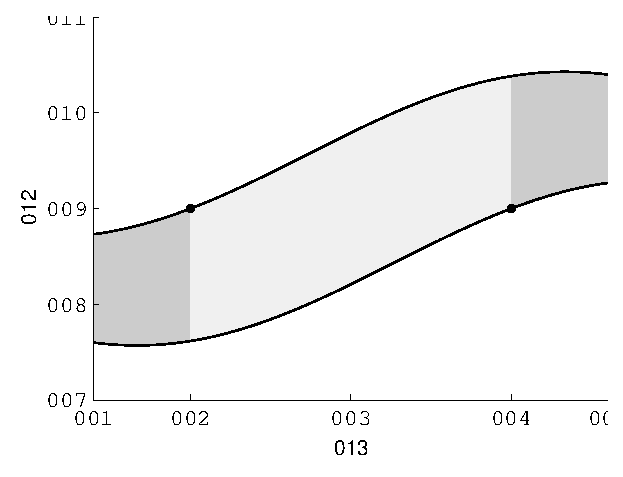
\includegraphics[width=.5 \linewidth,trim = 0cm 0cm 0cm 0cm]{3_Maximaler_Knickwinkel_Laenge1_Paper.eps}\label{fig:Maximaler_Knickwinkel_Vergleich_kurz}} %\\[3ex]
	% Zweite Figure	
	\input{../Bilder/3_Maximaler_Knickwinkel_Laenge2_Paper.tex}
    \subfigure[langer Anhänger ($l_t > l_{t,\text{lim}}$)]{
		\includegraphics[width=.5 \linewidth,trim = 0cm 0cm 0cm 0cm]{3_Maximaler_Knickwinkel_Laenge2_Paper.eps}\label{fig:Maximaler_Knickwinkel_Vergleich_lang}}
	% Beschriftung
    \caption[Realisierbare Knickwinkeländerungsraten]{Durch maximalen und minimalen Lenkeinschlag  (obere und untere schwarze Linie) gegebener Bereich (grau) der Knickwinkeländerungsrate in Abhängigkeit des Knickwinkels \citeltex{werling2014anhaenger}}
    \label{fig:Maximaler_Knickwinkel_Vergleich}
\end{figure}


Zur Festlegung von $\Delta\psi_\text{max}$ wiederum muss der für die Fahrzeug- und Anhängergeometrie zulässige Maximalknickwinkel $\Delta\psi_\text{max,geom}$ aus den Gespannparametern bestimmt werden. Er ist mit dem durch den zulässigen Lenkwinkel $\delta_{\text{max},\text{stat}}$ stationär stabilisierbaren Knickwinkel $\Delta\psi_\text{max,stat}$ mittels
\begin{align}
	\Delta\psi_\text{max} = \text{min}(\Delta\psi_\text{max,geom}, \Delta\psi_\text{max,stat})
\end{align}
 zu vergleichen. Letzterer wird für Anhänger mit $l_t \leq l_{\rm t,lim}$,
\begin{equation*}
	l_{\rm t,lim} = \sqrt{\frac{l_v^2}{\tan^2\delta_{\text{max},\text{stat}}}+l_c^2}, %\label{eq:assistiert:ltlim}
\end{equation*}
erhalten (vgl.\ Abb.\,\ref{fig:Maximaler_Knickwinkel_Vergleich_kurz}), indem wieder
die Nulldynamik mit $\kappa_{t,d} \equiv \kappa_{t}$ herangezogen wird. Gleichsetzen von \eqref{eq:assistiert:kruemmung} zum maximal zulässigen Lenkwinkel $\delta_{\text{max},\text{stat}}$ und  \eqref{eq:kappatdmax} liefert nach einigen Umformungen den maximal zulässigen Knickwinkel
\begin{equation}
	\Delta\psi_{\text{max},\text{stat}} = \arccos\left( -c_1 + \sqrt{c_2 + c_1^2} \right) \label{equ:eta_max_stat}
\end{equation}
mit
\begin{equation*}
	c_1 = \frac{l_c l_t \tan^2\delta_{\text{max},\text{stat}}}{l_v^2 + l_c^2 \tan^2\delta_{\text{max},\text{stat}}}, \quad
	c_2 = \frac{l_v^2 - l_t^2 \tan^2\delta_{\text{max},\text{stat}}}{l_v^2 + l_c^2 \tan^2\delta_{\text{max},\text{stat}}}.
\end{equation*}


\begin{figure}[ht]
	\centering
	% Erste Figure	
	\def\xlabel{$l_t$ in \unit{m}}
	\def\ylabel{$\Delta\psi_\text{max,geom}, \Delta\psi_\text{max,stat}$ in \unit{rad}}	
	% Generated using matlabfrag
% Version: v0.6.16
% Version Date: 04-Apr-2010
% Author: Zebb Prime
%
%% <text>
%
\providecommand\matlabtextA{\color[rgb]{0.000,0.000,0.000}\fontsize{10}{10}\selectfont\strut}%
\psfrag{013}[cc][cc]{\matlabtextA zulässiger Knickwinkel}%
%
\providecommand\matlabtextB{\color[rgb]{0.000,0.000,0.000}\fontsize{11}{11}\selectfont\strut}%
\psfrag{011}[bc][bc]{\matlabtextB \xlabel}%
\psfrag{012}[tc][tc]{\matlabtextB \ylabel}%
%
%% </text>
%
%% <xtick>
%
\def\matlabfragNegXTick{\mathord{\makebox[0pt][r]{$-$}}}
%
\psfrag{000}[ct][ct]{\matlabtextB 0}%
\psfrag{001}[ct][ct]{\matlabtextB 1}%
\psfrag{002}[ct][ct]{\matlabtextB 2}%
\psfrag{003}[ct][ct]{\matlabtextB 3}%
\psfrag{004}[ct][ct]{\matlabtextB 4}%
\psfrag{005}[ct][ct]{\matlabtextB $l_{t,\text{lim}}$}%
\psfrag{006}[ct][ct]{\matlabtextB 5}%
%
%% </xtick>
%
%% <ytick>
%
\psfrag{007}[rc][rc]{\matlabtextB 0}%
\psfrag{008}[rc][rc]{\matlabtextB $\frac{\pi}{4}$}%
\psfrag{009}[rc][rc]{\matlabtextB $\frac{\pi}{2}$}%
\psfrag{010}[rc][rc]{\matlabtextB $\frac{3\pi}{4}$}%
%
%% </ytick>
	%\renewcommand{\matlabtextA}{\footnotesize}
	%\renewcommand{\matlabtextB}{\scriptsize}
	\renewcommand{\matlabtextB}{\small}
	\includegraphics[width=.7 \linewidth,trim = 0cm 0cm 0cm 0cm]{3_Maximaler_Knickwinkel_Paper.eps}
	% Beschriftung
    \caption[Zulässiger Absolutknickwinkel]{Zulässiger Absolutknickwinkel $\Delta\psi_\text{max,stat}$ (schwarz) in Abhängigkeit der Anhängerlänge sowie konstruktiver Grenzwert $\Delta\psi_\text{max,geom}$ (gestrichelt) für typische Fahrzeugparameter \citeltex{werling2014anhaenger}}
    \label{fig:Maximaler_Knickwinkel}
\end{figure}


Da eine Krümmungsänderung des Anhängers immer mit einer gegensinnigen Lenkbewegung eingeleitet wird, muss $\delta_{\text{max},\text{stat}}$ merklich kleiner gewählt werden als $\delta_{\text{max}}$. Ansonsten dauert der Übergang aufgrund des dynamischen Sättigungsverhaltens zu lange. \\ %(s.\ später Abschn.\,\ref{sec:eval_kruemmungsstab}). \\
Für Anhänger mit $l_t > l_{\rm t,lim}$ hingegen existiert keine reelle Lösung von \eqref{equ:eta_max_stat}, was sich praktisch darin äußert, dass $\delta_{\text{max},\text{stat}}$ grundsätzlich ausreicht, den Anhänger zu stabilisieren (s.\ Abb.\,\ref{fig:Maximaler_Knickwinkel_Vergleich_lang}), sodass der konstruktive Grenzwert $\Delta\psi_\text{max,geom}$ (s.\ gestrichelte Linie in Abb.\,\ref{fig:Maximaler_Knickwinkel}) den maximalen Knickwinkel beschränkt.

%Bei Fahrt mit stationärem Knickwinkel fallen in Abb.\,\ref{fig:KESM_Gespann} $\mathrm{MP}_t$ und $\mathrm{MP}_v$ zu einem gemeinsamen Momentanpol $\mathrm{MP}$ zusammen. Wird nun in diesem stationären Fall die Anhängerdeichsellänge $l_t$ gedanklich verlängert, so wandert der Anhängerachsmittelpunkt in Richtung $\mathrm{MP}$, bis auch diese beiden Punkte zusammenfallen und sich das Fahrzeug um den stationären Anhängerachsmittelpunkt dreht.

%Geometrischer Maximalknickwinkel $\Delta\psi_\text{max,geom}$ und stationär stabilisierbarer Maximalknickwinkel $\Delta\psi_\text{max,stat}$
%\begin{align}
	%\Delta\psi_\text{max} = \text{min}(\Delta\psi_\text{max,stat}, \Delta\psi_\text{max,geom})
%\end{align}
%Mit $\Delta\psi' = 0$ und $\Delta\psi = \Delta\psi_\text{max}$ liefert die erste Zeile von \eqref{equ:zeittransformiertes_system_dynamics} nach Auflösen und
%einsetzen in 
%\eqref{eq:assistiert:kruemmung}
%\begin{align}
	%\kappa_{t,\text{max,stat}} = \kappa(\Delta\psi_\text{max},\delta(\Delta\psi_\text{max})).
%\end{align}

\subsubsection{Automatische Korrektur der manuellen Krümmungsvorgaben}
Zur Vermeidung der mit zu hohen Sollkrümmungsvorgaben $\kappa_\text{man}$ des Fahrers verbundenen Instabilität muss jetzt lediglich sichergestellt werden, dass diese zu jedem Zeitpunkt die zuvor hergeleiteten hinreichenden Bedingungen \eqref{equ:kappa_max_inst} und \eqref{eq:kappatdmax}   einhalten. Eine gleichermaßen einfache wie für den Fahrer intuitive Möglichkeit ist hierfür die Zwischenschaltung eines statischen und  dynamischen Sättigungsglieds, und zwar
\newcommand{\sat}[2]{\text{sat}_{#1}^{#2}}
\begin{align}
	 \negspace \kappa_{t,d} = \sat{-\kappa_{t,\text{max,inst}(\Delta\psi)}}{\kappa_{t,\text{max,inst}(\Delta\psi)}} \left(\, \sat{-\kappa_{t,\text{max,stat}}}{\kappa_{t,\text{max,stat}}}(\kappa_\text{man})\,\right).
\end{align}

Eine Übersichtsdarstellung der Reglerstruktur kann Abb.\,\ref{fig:KrAblauf} entnommen werden.

\begin{figure}[ht]
	\centering
   \psfrag{boxeins}[cc][cc][0.8]{\eqref{eq:fzgmodell:psi_v_dot}\,-\,\eqref{eq:assistiert:delta_dot}}
	\psfrag{boxzwei}[cc][cc][1.0]{\eqref{equ:linearisierendeRueckfuehrungKruemmung}}
	\psfrag{boxdrei}[cc][cc][1.0]{\eqref{equ:zustandsregler_kruemmung}}
	\psfrag{boxvier}[cc][cc][1.0]{\eqref{equ:trafo_kruemmung}}
	\psfrag{dietextboxeins}[cl][cl][1.0]{\parbox[st]{3cm}{nichtlineare\\Systemdynamik}}
	\psfrag{dietextboxzwei}[cl][cl][1.0]{\parbox[t]{3cm}{linearisierende\\Rückführung}}
	\psfrag{dietextboxdrei}[cl][cl][1.0]{\parbox[t]{3cm}{linearer\\Zustandsregler}}
	\psfrag{dietextboxvier}[cl][cl][1.0]{\parbox[t]{3cm}{Zustands-\\transformation}}
	\psfrag{dietextboxfunf}[cl][cl][1.0]{\parbox[t]{3cm}{dynamische\\Sättigung}}
	\psfrag{dietextboxsechs}[cl][cl][1.0]{\parbox[t]{3cm}{statische\\Sättigung}}
	\psfrag{labeleins}[cl][cl][1.0]{$u$}
	\psfrag{labelzwei}[cl][cl][1.0]{$\nu$}
	\psfrag{labeldrei}[cl][cl][1.0]{$\xi$}
	\psfrag{labelvier}[cl][cl][1.0]{$[\kappa_{t,d},\kappa_{t,d}']^\T$}
	\psfrag{labelfunf}[cl][cl][1.0]{}
	\psfrag{labelsechs}[cl][cl][1.0]{$\kappa_\text{man}$}
	\psfrag{lablA}[cr][cr][1.0]{$\begin{bmatrix}\Delta\psi\\\delta\end{bmatrix}$}
	\includegraphics[width=.5 \linewidth,trim = 0cm 0cm 0cm 0cm]{3_Kruemmungsfolgeregelung_Ablauf.eps}
    \caption[Aufbau der asymptotischen Krümmungsfolgeregelung]{Aufbau der asymptotischen Krümmungsfolgeregelung \citeltex{werling2014anhaenger}}
    \label{fig:KrAblauf}
\end{figure}

%\subsection{Pfadfolgeregelung für den Anhänger} \label{sec:pfadstab}
%\subsubsection{Systemerweiterung um Pfadfolgedynamik} \label{sec:pfaderweiterung}
%Im Unterschied zum vorherigen Regelungsziel, den Krümmungsfehler des Anhängerkurses zu minimieren, wird nun auf die Stabilisierung des Anhängers entlang einer Sollkurve abgezielt. Entsprechend Abb.\,\ref{fig:Pfadfolgeregelung} ist hierzu eine Erweiterung der Systembeschreibung um drei Zustände erforderlich. Diese sind der vorzeichenbehaftete Abstand $d$, die Bogenlänge $s_p$, über die der Sollpfad $\Gamma(s_p)$ parametriert ist, und die Fahrzeugorientierung $\psi_v$.
%\begin{figure}
	%\centering
    %\psfrag{MPc}[cl][cl][1.0]{$\mathrm{MP}_p$}
	%\psfrag{d}[cc][cc][1.0]{$d$}
	%\psfrag{vt}[rb][rb][1.0]{$\boldsymbol v_t$}
	%\psfrag{psit}[rt][rt][1.0]{$\psi_t$}
	%\psfrag{sc}[lt][lt][1.0]{$s_p$}
	%\psfrag{psic}[rc][rc][1.0]{$\psi_p$}
	%\psfrag{kc}[lc][lc][1.0]{$\dfrac{1}{\kappa_p}$}
	%\psfrag{rt}[br][br][1.0]{$\boldsymbol r_t$}
	%\psfrag{rc}[tr][tr][1.0]{$\boldsymbol r_p$}
	%\psfrag{Gamma}[rb][rb][1.0]{$\Gamma(s_p)$}
  %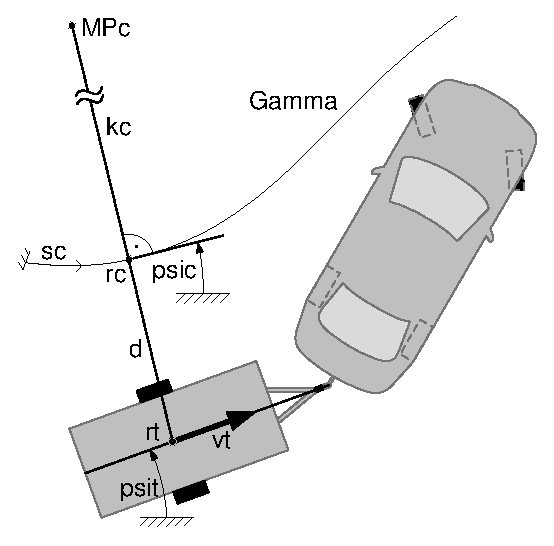
\includegraphics[width=.7 \linewidth,trim = 0cm 0cm 0cm 0cm]{3_PfadfolgeregelungPaper.eps}
    %\caption{Geometrische Zusammenhänge der Pfadfolgeregelung}
    %\label{fig:Pfadfolgeregelung}
%\end{figure}
%Die Dynamik von $\psi_v$ wird durch \eqref{eq:fzgmodell:psi_v_dot} beschrieben, die der anderen Zustände durch 
%\begin{subequations}
%\begin{align}
	%\dot{s}_p 	& = v_t \frac{\cos\left(\psi_t - \psi_p(s_p)\right)}{1 - d \kappa_p(s_p)} \label{eq:automatisch:scdot} \\
	%\dot{d} 	 	& = v_t \sin\left(\psi_t - \psi_p(s_p)\right) \label{eq:automatisch:ddot} %\\ 	\dot{\psi}_v	& = v_v \frac{\tan\delta}{l_v}
%\end{align}
%\end{subequations}
%in Abhängigkeit der Pfadorientierung $\psi_p(s_p)$ und "~krümmung $\kappa(s_p)$ des Projektionspunkts $\boldsymbol r_p$ (vgl.\ \cite{atSonderheft08}). Zur kompakten Darstellung wird anstelle des Knickwinkels $\Delta\psi$ nun die Anhängerorientierung $\psi_t$ verwendet. Damit stellt sich der neue Systemzustand als $\bldx = [s_p, d, \psi_v, \psi_t, \delta]^\T$ dar. \\
%Bei kleinen Abweichungen $d$ und $\psi_p-\psi_t$ des Anhängers vom Sollpfad sowie Sollkrümmungen mit $\kappa_p \ll \nicefrac{1}{d}$
%ergibt sich für die Darstellung \eqref{equ:zeittransformiertes_system} in guter Näherung
%\begin{align*}
	%\negspace\negspace
	%\boldsymbol f(\boldsymbol x) &= 
		%\begin{bmatrix}
			%-1 \\[1ex]
			%\psi_p - \psi_t \\[1ex]
			%-\dfrac{\tan \delta}{l_v \cos(\psi_v\!-\!\psi_t)+l_c \sin(\psi_v\!-\!\psi_t)\tan \delta} \\[3ex]
			%\dfrac{-l_v \sin(\psi_v\!-\!\psi_t)+l_c \cos(\psi_v\!-\!\psi_t)\tan \delta}{l_t \left[l_v \cos(\psi_v\!-\!\psi_t)+l_c \sin(\psi_v\!-\!\psi_t)\tan \delta\right]} \\[3ex]
			%\dfrac{l_v \delta}{T v_v \left[l_v \cos(\psi_v\!-\!\psi_t)+l_c \sin(\psi_v\!-\!\psi_t)\tan \delta\right]}
		%\end{bmatrix}
	%\end{align*}
%und
%\begin{align*}
	%\negspace\negspace
	%\boldsymbol g(\boldsymbol x) &= 
		%\begin{bmatrix}
			%0 \\
			%\vdots \\
			%0 \\[1ex]
			%- \dfrac{l_v}{T v_v \left[l_v \cos(\psi_v\!-\!\psi_t)+l_c \sin(\psi_v\!-\!\psi_t)\tan \delta\right]}
		%\end{bmatrix},
%\end{align*}
%sowie die zu minimierende Pfadabweichung
%\begin{align*}
	%h(\bldx) = d.
%\end{align*}
%
%\subsubsection{Entwurf der Pfadfolgeregelung} \label{sec:pfadstab_entwurf}
%Aufgrund des gegenüber Abschn.\,\ref{sec:kruemmungsstab} modifizierten Sys\-tems stellen sich die ersten drei Ableitungen des Ausgangs nun als
%\begin{align*}
%\negspace\negspace
	%h'(\bldx) &= \Lie_f h(\bldx) + \underbrace{\Lie_gh(\boldsymbol x)}_{=0} u= \psi_p(s_p) - \psi_t \\[1ex]
%\negspace\negspace	
	%h''(\bldx) &= L^2_f h(\bldx) +  \underbrace{\Lie_g\Lie_fh(\boldsymbol x)}_{=0} u = \\[1ex]
%\negspace\negspace
	%& \negspace-\kappa_p(s_p)+\frac{l_v\sin(\psi_v\!-\!\psi_t)-l_c\cos(\psi_v\!-\!\psi_t)\tan \delta}{l_t \left[l_v \cos(\psi_v\!-\!\psi_t)+l_c\sin(\psi_v\!-\!\psi_t)\tan \delta\right]}\\[3ex]
	%\negspace\negspace
	%h'''(\bldx) &= \Lie_f^3h(\bldx) + \underbrace{\Lie_g\Lie_f^2h(\boldsymbol x)}_{\neq 0} u  =   -\kappa_p^\prime(s_p) + \\[1ex]
	%&\negspace\negspace\negspace\!\!\frac{\!\left[l_v^2\!+\!l_c^2\tan^2 \!\delta\right]\!\!\left[-l_t\!\tan\!\delta\!\!l_v \!\sin (\psi_v\!-\!\psi_t)\!-\!l_c\! \cos (\psi_v\!-\!\psi_t)\!\tan \!\delta\right]}{l_t^2\left[l_v\cos (\psi_v\!-\!\psi_t)+l_c\sin (\psi_v\!-\!\psi_t)\tan \delta\right]^3}\\[1ex]
	%& \negspace\negspace\negspace-\frac{l_v^2l_c\delta}{l_tTv_v\cos^2\!\delta\left[l_v\cos(\psi_v\!-\!\psi_t)+l_c\sin(\psi_v\!-\!\psi_t)\tan \delta\right]^3} \\[1ex]
	%& \negspace\negspace\negspace +\frac{l_v^2l_c}{l_tTv_v\cos^2\!\delta\left[l_v\cos(\psi_v\!-\!\psi_t)+l_c\sin(\psi_v\!-\!\psi_t)\tan \delta\right]^3} u \\[2ex]
	%\negspace\negspace\negspace =: \nu
%\end{align*}
%dar (vgl.\ mit \eqref{equ:ersteAbleitung_kruemmung}), sodass der relative Grad auf drei angestiegen ist. Mit dem Rückführungsgesetz
%\begin{align}
%\nonumber
%\negspace\negspace
	%u &= \frac{1}{\Lie_g\Lie_f^2h(\boldsymbol x)}\left[-\Lie_f^3h(\boldsymbol x) + \nu \right] = \\[1ex]
%\nonumber
%\negspace\negspace
		%&\frac{l_tTv_v\cos^2\!\delta}{l_v^2 l_c}\\[1ex]
%\nonumber
%\negspace\negspace
		%&\cdot\Biggl[ \left[l_v\cos (\psi_v\!-\!\psi_t)+l_c\sin (\psi_v\!-\!\psi_t)\tan \delta\right]^3 [\kappa'_{p}(s_p)+\nu] 	\\[1ex]
		%\negspace\negspace
		%\nonumber
		%& - \frac{\left[l_v^2\!+\!l_c^2\tan^2\delta\right]}{l_t^2} \\
	  %\nonumber
		%\negspace\negspace
		%& \cdot \left[-l_t\tan \delta+l_v \sin (\psi_v\!-\!\psi_t)-l_c \cos (\psi_v\!-\!\psi_t)\tan \delta\right]\Biggr] \\[1ex]
		%\negspace\negspace
			%& + \delta \;, \label{equ:linearisierendeRueckfuehrungPfad}
%\end{align}
%$l_v,l_c,l_t > 0$ und $|\delta| < \nicefrac{\pi}{2}$,
%liefert die Koordinatentransformation 
%\begin{equation}
	%\boldsymbol \xi^\T = [\xi_1, \xi_2, \xi_3] = [h(\bldx), \Lie_f h(\bldx), \Lie^2_fh(\bldx)] \label{equ:trafo_pfad}
%\end{equation}
%das Integratorsystem
%\begin{align*}
	%\xi_1' = \xi_2, \quad \xi_2' = \xi_3, \quad \xi_3' = \nu; \quad \boldsymbol \xi(0) = \boldsymbol 0,
%\end{align*}
%welches sich durch
%\begin{equation}
	%\nu = -k_1 \xi_1 - k_2\xi_2 - k_3 \xi_3 \quad \label{equ:zustandsregler_pfad}
%\end{equation}
%mit Hurwitz-Koeffizienten $k_1,k_2,k_3$ %(s.\ später Abschn.\,\ref{sec:eval})
%asymptotisch stabilisieren lässt.
%
%In den Koordinaten $[\eta_1, \eta_2] = [s_p, \psi_v - \psi_t]$ stellt sich die interne Dynamik als
%\begin{align}
	%\eta_1' &= -1 \label{equ:autonome_nd}\\
	%\eta_2' &=  -\dfrac{1}{l_c}\bigl[\sin \eta_2 - \left[\kappa_p+\xi_3\right]\left[l_c+l_t\cos \eta_2\right]\bigr], \label{equ:zweiterTeil_nd}
%\end{align}
%$\boldsymbol \eta(0) = [s_{p0}, \Delta\psi_0]^\T$, dar. Die Teildynamik \eqref{equ:autonome_nd} ist instabil, was allerdings die Anwendung auch erfordert, da sich der Kurvenparameter $s_p$ entsprechend der hier gewählten Definition genau entgegen der unabhängigen Variable $s_t$ bewegt, s.\ Abb.\,\ref{fig:Pfadfolgeregelung}. Was die Teildynamik \eqref{equ:zweiterTeil_nd} betrifft, so ist sie für $\kappa_p = \kappa_{t,d}$ identisch mit der aus Abschn.\,\ref{sec:kruemmungsstab_entwurf}, womit die dortigen Ergebnisse als Anforderungen an die Sollkurve $\Gamma(s_p)$ übernommen werden können.
%
%Wie Abb.\,\ref{fig:PfAblauf} zu entnehmen ist, sind damit alle zur asymptotischen Pfadfolgeregelung erforderlichen Formeln vorhanden, und es verbleibt, diese zusammen mit der Krümmungsfolgeregelung des vorherigen Abschnitts zu erproben.
%
%\begin{figure}
	%\centering
    %\psfrag{boxeins}[cc][cc][1.0]{\eqref{eq:fzgmodell:psi_v_dot}, \eqref{eq:fzgmodell:psi_t_dot}, \eqref{eq:assistiert:delta_dot}}
	%\psfrag{boxzwei}[cc][cc][1.0]{\eqref{equ:linearisierendeRueckfuehrungPfad}}
	%\psfrag{boxdrei}[cc][cc][1.0]{\eqref{equ:zustandsregler_pfad}}
	%\psfrag{boxvier}[cc][cc][1.0]{\eqref{equ:trafo_pfad}}
	%\psfrag{boxfunf}[cc][cc][1.0]{$\Gamma (s_p)$}
	%\psfrag{dietextboxeins}[cl][cl][1.0]{\parbox[t]{3cm}{nichtlineare\\Systemdynamik}}
	%\psfrag{dietextboxzwei}[cl][cl][1.0]{\parbox[t]{3cm}{linearisierende\\Rückführung}}
	%\psfrag{dietextboxdrei}[cl][cl][1.0]{\parbox[t]{3cm}{linearer\\Zustandsregler}}
	%\psfrag{dietextboxvier}[cl][cl][1.0]{\parbox[t]{3cm}{Zustands-\\transformation}}
	%\psfrag{dietextboxfunf}[cl][cl][1.0]{\parbox[t]{3cm}{Sollpfad}}	
	%\psfrag{labeleins}[cl][cl][1.0]{$u$}
	%\psfrag{labelzwei}[cl][cl][1.0]{$\nu$}
	%\psfrag{labeldrei}[cl][cl][1.0]{$\begin{bmatrix}\xi_1,\xi_2,\xi_3\end{bmatrix}^\T$}
	%\psfrag{labelvier}[cl][cl][1.0]{$[d,\psi_p,\kappa_{p},\kappa_p']^\T$}
	%\psfrag{labelfunf}[cl][cl][1.0]{}
	%\psfrag{labelsechs}[cl][cl][1.0]{$\kappa_\text{man}$}
	%\psfrag{lablA}[cr][cr][1.0]{$s_p$}
	%\psfrag{lablB}[cc][cc][1.0]{$\begin{bmatrix}\psi_v\\\psi_t\\\delta\end{bmatrix}$}
  %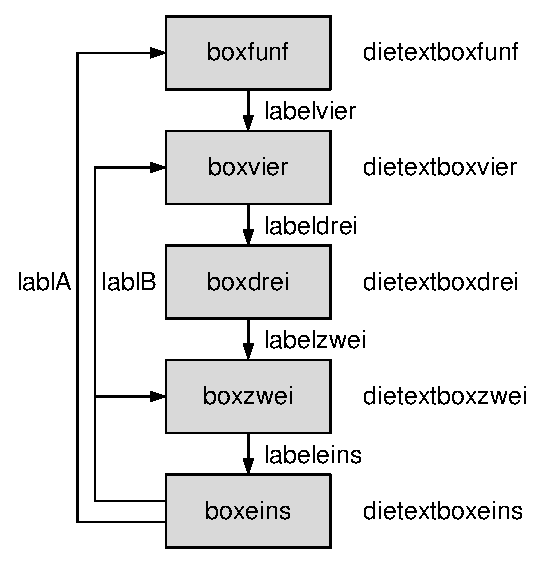
\includegraphics[width=.7 \linewidth,trim = 0cm 0cm 0cm 0cm]{3_Pfadfolgeregelung_Ablauf.eps}
    %\caption{Aufbau der asymptotischen Pfadfolgeregelung}
    %\label{fig:PfAblauf}
%\end{figure}


\subsection{Implementierung und Evaluation im Realversuch}\label{sec:eval_trailer}
%\subsubsection{Prototypische Umsetzung}
Der Funktionsnachweis erfolgt auf einem BMW 5er der sechsten Generation, %, s.\ Abb.\,\ref{fig:foto}, 
welcher zur Messung des Knickwinkels mit einer modifizierten Anhängerkupplung ausgestattet ist. Die Regelungsalgorithmen sind in Simulink/Embedded Matlab umgesetzt und laufen mit einer Zykluszeit von $\unit[10]{ms}$ auf einer dSpace Autobox.
% , s.\ Abb.\,\ref{fig:kupplung}. 
%\begin{figure}[ht]
	%\centering
  %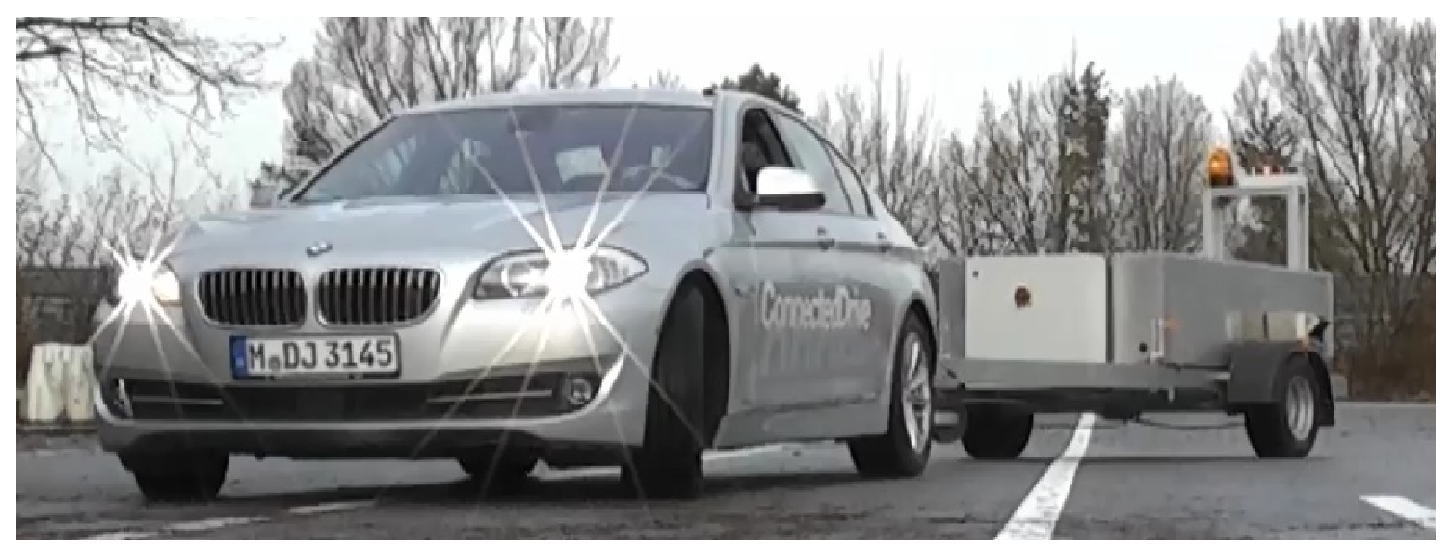
\includegraphics[width=0.8 \linewidth,trim = 0cm 0cm 0cm 0cm]{3_GespannFoto.eps}	
    %\caption{Versuchsfahrzeug mit Anhänger}
    %\label{fig:foto}
%\end{figure}

%Die Ansteuerung der elektrischen Serienservolenkung erfolgt über eine Modifikation der Steuergerätesoftware. Darüber hinaus wird zur Eigenlokalisierung der serienmäßige Gierraten- und Geschwindigkeitssensor unter Annahme verschwindend kleiner Schräglaufwinkel der Hinterachse aufintegriert (s.\ \zB \cite{borenstein1997}). 
%Ferner erfolgt bei der Pfadstabilisierung die zur Bestimmung von $s_p$ erforderliche Projektion über den in \cite{irle2009zwei} beschriebenen Bi-Kurven-Ansatz. Die Regelungsalgorithmen selbst sind in Simulink/Embedded Matlab umgesetzt und laufen mit einer Zykluszeit von $\unit[10]{ms}$ auf einer dSpace Autobox.

Vier Instantanaufnahmen des Gespanns aus der Vogelperspektive sind in Abb.\,\ref{fig:Auswertung_Kruemmung_Fahrversuch_draufsicht} abgebildet, welchen die in Abschn.\,\ref{sec:koppelnavi} auf S.\,\pageref{sec:koppelnavi} beschriebenen Eigenlokalisierung zugrunde liegt. Zur Verdeutlichung der Gespannbewegung zieht der Anhängerachsmittelpunkt eine schwarze Spur und sowohl die Soll- (grau) als auch die Ist-Krümmung (schwarz) wird als gestricheltes Kreissegment dargestellt. In Abb.\,\ref{fig:Auswertung_Kruemmung_Fahrversuch}  befinden sich dazu die wichtigsten Zeitsignalverläufe, wobei die zu den vier Instantanaufnahmen zugehörigen Zeitpunkte durch senkrechte graue Striche markiert sind.


%\subsubsection{Ergebnisse der Krümmungsstabilisierung} \label{sec:eval_kruemmungsstab}
%
\begin{figure}[ht]
	\centering
	% Generated using matlabfrag
% Version: v0.6.16
% Version Date: 04-Apr-2010
% Author: Zebb Prime
%
%% <text>
%
\providecommand\matlabtextA{\color[rgb]{0.000,0.000,0.000}\fontsize{10}{10}\selectfont\strut}%
\psfrag{000}[bc][bc]{\matlabtextA $t=37\unit{s}$}%
\psfrag{001}[bc][bc]{\matlabtextA $t=25\unit{s}$}%
\psfrag{002}[bc][bc]{\matlabtextA $t=15\unit{s}$}%
\psfrag{003}[bc][bc]{\matlabtextA $t=2\unit{s}$}%
%
%% </text>
	\renewcommand{\matlabtextA}{\scriptsize}
	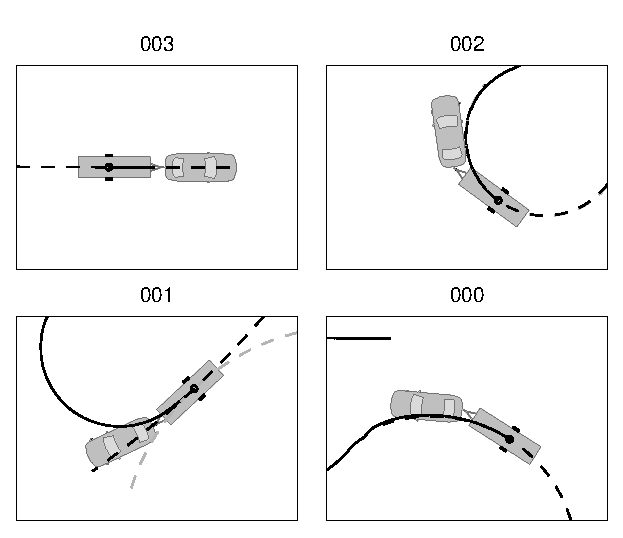
\includegraphics[width=.9 \linewidth,trim = 0cm 0cm 0cm 0cm]{3_Auswertung_Kruemmung_Fahrversuch_Paper_birdview.eps}		
	\def\xlabel{$t$ in \unit{s}}
    \caption[Draufsichten des Fahrversuchs mit Krümmungsregler]{Draufsichten des Fahrversuchs mit Krümmungsregler \citeltex{werling2014anhaenger}}
    \label{fig:Auswertung_Kruemmung_Fahrversuch_draufsicht}
	\end{figure}
	


Der Fahrversuch beginnt mit dem Einlegen des Rückwärtsgangs, was automatisch die Sollkrümmung mit dem aktuellen Lenk- und Knickwinkel (beide ungefähr Null, s.\ $\delta$- und $\Delta\psi$-Signal in Abb.\,\ref{fig:Auswertung_Kruemmung_Fahrversuch}) abgleicht und damit die Krümmungsstabilisierung ruckfrei aktiviert. Anschließend beschleunigt der Fahrer auf $v_v\approx \unitfrac[-2]{m}{s}$, ohne dabei die Hände am Steuer zu haben, sodass der Regler die Sollkrümmung frei stabilisieren kann (s.\ Aufnahme oben links). Bei $t\approx \unit[5]{s}$ "`lenkt"' der Fahrer durch gleichmäßiges Rotieren eines Drehknopfes den Anhänger in eine Linkskurve (s.\ Aufnahme oben rechts). Während der Realisierung des hierfür erforderlichen stetigen Krümmungsübergangs ist das typische Ein- und Gegenlenken im $\delta$-Signal erkennbar. Ab $t\approx \unit[10]{s}$ bewegt sich das Fahrzeuggespann für $\unit[10]{s}$ auf einer Kreisbahn mit konstantem Radius -- ohne dass die Sättigung der manuellen Krümmungsvorgabe an der stationären Maximalkrümmung (s. dunkelgrauer Bereich) aktiv wird. Daraufhin wird die Sollkrümmung (graue Linie im zweiten Signalverlauf von oben) durch Gegenrotation des Drehknopfes zügig erhöht, was zur Folge hat, dass jetzt die instantane Krümmungssättigung aktiv wird (s.\ hellgrauer Bereich ober- und unterhalb von $\kappa_t$), welche verhindert, dass die Lenkung ihre Regelreserve aufbraucht (s. Lenkwinkelverlauf). Der Sachverhalt wird auch in der Draufsicht unten links für $t=\unit[25]{s}$ durch das merkliche Abweichen der tatsächlichen (schwarz gestrichelten) von der manuell vorgegebenen Krümmung (grau gestrichelt) verdeutlicht.

	\begin{figure}[ht]
	\centering
	% Generated using matlabfrag
% Version: v0.6.16
% Version Date: 04-Apr-2010
% Author: Zebb Prime
%
%% <text>
%
\providecommand\matlabtextA{\color[rgb]{0.000,0.000,0.000}\fontsize{10}{10}\selectfont\strut}%
\psfrag{000}[bc][bc]{\matlabtextA $t=37\unit{s}$}%
\psfrag{001}[bc][bc]{\matlabtextA $t=25\unit{s}$}%
\psfrag{002}[bc][bc]{\matlabtextA $t=15\unit{s}$}%
\psfrag{003}[bc][bc]{\matlabtextA $t=2\unit{s}$}%
%
%% </text>
	\renewcommand{\matlabtextA}{\scriptsize}
  %  \subfigure{\includegraphics[width=0.96\columnwidth]{Auswertung_Kruemmung_Fahrversuch_Paper_birdview}}			
	%\\[2ex]
	%\subfigure{\includegraphics[width=0.96\columnwidth]{Auswertung_Kruemmung_Fahrversuch_Paper_birdview}}		
	\def\xlabel{$t$ in \unit{s}}
	\def\ylabelA{$\delta$ in \unit{rad}}	
	\def\ylabelB{$v_v$ in \unitfrac{m}{s}}	
	\def\ylabelC{$\Delta\psi$ in \unit{rad}}		
	\def\ylabelD{$\kappa_t$ in \unit{m$^{-1}$}}	
	\def\ylabelE{$e_\kappa$ in \unit{m$^{-1}$}}		
	\input{../bilder/3_Auswertung_Kruemmung_Fahrversuch_Paper_signals.tex}
	\renewcommand{\matlabtextA}{\scriptsize}
  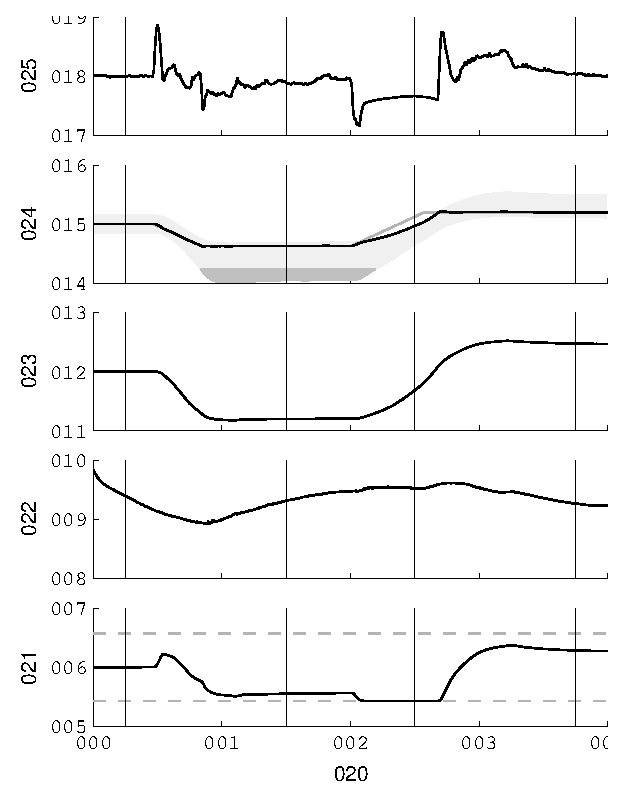
\includegraphics[width=.7 \linewidth,trim = 0cm 0cm 0cm 0cm]{3_Auswertung_Kruemmung_Fahrversuch_Paper_signals.eps}
    \caption[Signalverläufe des Fahrversuchs mit Krümmungsregler] {Signalverläufe des Fahrversuchs mit Krümmungsregler \citeltex{werling2014anhaenger}}
    \label{fig:Auswertung_Kruemmung_Fahrversuch}
	\end{figure}
%	

Nach kurzer Zeit liegt die Sollkrümmung wieder innerhalb der sich dynamisch ändernden instantanen Krümmungssättigung, sodass die mittlerweile konstante Sollkrümmung (dunkelgrau) umgesetzt wird und eine Unterscheidung der Ist- und Sollkrümmung in der Draufsicht bereits nicht mehr möglich ist.

%Zum Funktionsnachweis und zur Demonstration der Einsatzmöglichkeit des Pfadfolgereglers durchfährt zunächst der Fahrzeugführer manuell einen S-förmigen Straßenabschnitt. Dabei werden bereits die Koordinaten des Anhängerachsmittelpunkts als Pfad (graue Linie in den Draufsichten in Abb.\,\ref{fig:Auswertung_Pfad_Fahrversuch_draufsicht}) aufgezeichnet. Anschließend legt er den Rückwärtsgang ein, lässt das Lenkrad los und gibt manuell Gas. Hierdurch beschleunigt das Fahrzeug rückwärts auf bis zu $v_v\approx -\unitfrac[2]{m}{s}$, während die Pfadfolgeregelung den Anhänger entsprechend des abgespeicherten Pfads und damit entlang der Straße stabilisiert. Da bei der Vorwärtsfahrt der Lenkwinkel nicht voll ausgeschöpft wurde, treten bei der Rückwärtsfahrt keine Stellgrößenbeschränkungen auf (s.\ $\kappa$-Signal innerhalb des zulässigen Bereichs in grau). Bei $t\approx \unit[37]{s}$ reduziert der Fahrer die Rückwärtsgeschwindigkeit und das Gespann kommt ca. $\unit[3]{s}$ später zum Stillstand.
%\subsubsection{Ergebnisse der Pfadfolgeregelung}
%\begin{figure}
	%\centering
	%\input{../bilder/3_Auswertung_Pfad_Fahrversuch_Paper_birdview}
	%\renewcommand{\matlabtextA}{\scriptsize}
  %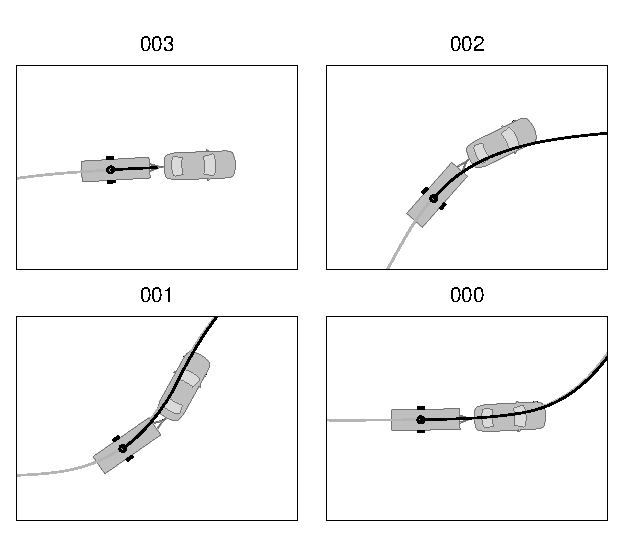
\includegraphics[width=.9 \linewidth,trim = 0cm 0cm 0cm 0cm]{3_Auswertung_Pfad_Fahrversuch_Paper_birdview.eps}
    %\caption{Draufsichten des Fahrversuchs mit Pfadstabilisierung}
    %\label{fig:Auswertung_Pfad_Fahrversuch_draufsicht}
%\end{figure}
%
%\begin{figure}
	%\centering
	%\def\xlabel{$t$ in $\unit{s}$}
	%\def\ylabelA{$\delta$ in $\unit{rad}$}	
	%\def\ylabelB{$v_v$ in $\unitfrac{m}{s}$}	
	%\def\ylabelC{$\Delta\psi$ in $\unit{rad}$}		
	%\def\ylabelD{$\kappa_t$ in $\unit{m^{-1}}$}	
	%\def\ylabelE{$d$ in $\unit{m}$}	
	%\input{../bilder/3_Auswertung_Pfad_Fahrversuch_Paper_signals}
	%\renewcommand{\matlabtextA}{\scriptsize}
  %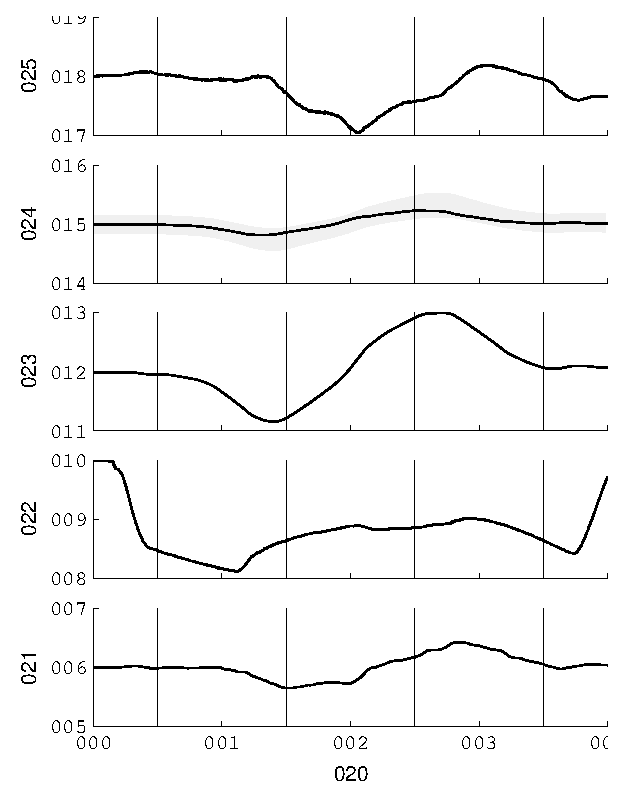
\includegraphics[width=.63 \linewidth,trim = 0cm 0cm 0cm 0cm]{3_Auswertung_Pfad_Fahrversuch_Paper_signals.eps}
  %\caption{Signalverläufe des Fahrversuchs mit Pfadstabilisierung}
  %\label{fig:Auswertung_Pfad_Fahrversuch}
%\end{figure}

%\subsubsection{Diskussion}
%Die Bedienung über Drehknopf gibt auch dem ungeübten Fahrer eine intuitive Möglichkeit, über automatisch eingeregelte Krümmungssollvorgaben den Anhänger zu manövrieren, welcher dann das Fahrzeug "`hinter sich herzieht"'.
%Dabei kann der Sättigung des Stellglieds und dem irreversiblen Abknicken des Anhängers effektiv entgegengewirkt werden, indem die Sollkrümmung vor Weitergabe an den Regler sowohl an den instantanen als auch an den stationären Grenzen gesättigt wird. Die Regelgenauigkeit (s.\ $e_\kappa$-Signal in Abb.\,\ref{fig:Auswertung_Kruemmung_Fahrversuch}) ist trotz ruhigen Lenkverhaltens auffallend hoch. Lediglich in Bereichen der Sollkrümmungsknicke treten geringfügige Abweichungen auf, welche dem beschränkten Lenkmoment der Aktorik geschuldet sind und durch geringfügiges Tiefpassfiltern der Sollkrümmung reduziert werden können.

%Die Aufzeichnung der Koppelposition der Vorwärtsbewegung ermöglicht in vielen Situationen wie dem Befahren von Einfahrten die kurzzeitige Querstabilisierung des zurücksetzenden Gespanns.
%Während der Fahrt muss hierbei der entlastete Fahrer das Verkehrsgeschehen auf dynamische Hindernisse überwachen und ggf.\ darauf durch Anpassung der Längsgeschwindigkeit reagieren bzw.\ im schlimmsten Fall auf den Modus der Krümmungsstabilisierung zurückgreifen. Aufgrund der Verfügbarkeit von genauen Raddrehzahl- und Gierratensensoren ist die Eigenlokalisierung für eine Strecke im für die Praxis wichtigen Bereich von $50-\unit[100]{m}$ hinreichend genau; die Stabilisierung des Gespanns über längere Strecken erfordert allerdings die Fusion mit einer absoluten Positionsreferenz. \\
%Die Regelgenauigkeit der Pfadstabilisierung liegt mit unter $\unit[20]{cm}$ im tolerierbaren Bereich. Sie erfordert aber hierfür im Unterschied zur Krümmungsstabilisierung höhere Lenkaktivitäten (s. $\delta$-Signale), insbesondere bei Knickwinkelmessfehlern aufgrund von Bodenunebenheiten, was auf die gestiegene Anzahl der zu stabilisierenden Zustände zurückzuführen ist.


%\subsection{Zusammenfassung}\label{sec:zusammenfassung_trailer}
Insgesamt kann festgehalten werden, dass die Bedienung über den Drehknopf auch dem ungeübten Fahrer eine intuitive Möglichkeit verschafft, über automatisch eingeregelte Krümmungssollvorgaben den Anhänger zu manövrieren, welcher dann das Fahrzeug "`hinter sich herzieht"'.
Dabei kann der Sättigung des Stellglieds und dem irreversiblen Abknicken des Anhängers effektiv entgegengewirkt werden, indem die Sollkrümmung vor Weitergabe an den Regler sowohl an den instantanen als auch an den stationären Grenzen gesättigt wird. Die Regelgenauigkeit (s.\ $e_\kappa$-Signal in Abb.\,\ref{fig:Auswertung_Kruemmung_Fahrversuch}) ist trotz ruhigen Lenkverhaltens auffallend hoch. Lediglich in Bereichen der Sollkrümmungsknicke treten kleine Abweichungen auf, welche dem beschränkten Lenkmoment der Aktorik geschuldet sind und durch geringfügiges Tiefpassfiltern der Sollkrümmung reduziert werden können.

%In der vorliegenden Arbeit werden zwei Ausprägungen einer Assistenz für das Rückwärtsfahren von Pkw-Gespannen vorgestellt. \\
%Die erste Ausprägung ermöglicht dem Fahrer, während der Rückwärtsfahrt den Anhänger direkt über einen Drehknopf zu lenken. Das Fahrzeug vollführt dann die hierfür notwendigen Lenkbewegungen selbständig. Regelungstechnisch wird hierbei der Drehknopfwert als Soll-Kurskrümmung des Anhängers interpretiert, die ggf.\ zur Vermeidung der Lenkwinkelsättigungen und eines irreversiblen Abknickens dynamisch korrigiert wird. Das Ergebnis dient als Referenzsignal für eine auf Basis der exakten Ein-/Ausgangslinearisierung entworfene Folgeregelung, welche unter Berücksichtigung des gemessenen Differenzwinkels zwischen Fahrzeug und Anhänger das Lenkrad ansteuert. \\
%In der zweiten Ausprägung überlässt der Fahrer beim Rückwärtsfahren die komplette Querführung dem Assistenzsystem, das nun gegebenen Sollkurven, etwa die zuvor vorwärts zurückgelegte abgespeicherte Wegstrecke, mittels Lenkeingriffen eigenständig folgt. Der hierzu erforderliche Pfadfolgeregler wurde ebenfalls mittels exakter Ein-/Ausgangslinearisierung entworfen und stabilisiert neben der Krümmung auch die Position und Ausrichtung des Anhängers entsprechend des Sollpfadverlaufs.


Der Regler ist grundsätzlich dazu geeignet, einer modellprädiktiven Pfadoptimierung unterlagert  zu werden, sodass automatische Einparkmanöver mit Anhänger darstellbar sind. %Aufgrund der gegenüber dem alleinigen Fahrzeug gesteigerten Systemordnung und der variablen Anhängergeometrie erscheint eine Parametrierung von Standardmanövern über die Anfangsbedingungen, wie sie aktuell in Serienfahrzeugen eingesetzt wird, schwierig. 
In unstrukturierter Umgebung wie Parkplätzen eignen sich hierfür vor allem die im nächsten Kapitel vorgestellten Planungsmethoden. Die Planung in den flachen Koordinaten \cite{rouchon1993flatness1} kann aufgrund der algebraischen Beziehung zwischen Positions- und Ausrichtungsverlauf von Anhänger und Fahrzeug den Schlüssel zu einer schnellen Kollisionsüberprüfung \cite{zieglerfastcollision2010} darstellen.
%[Zukünftig Integration in bestehendes Sensorsystem von herkömmlichen Einparkassistenten, und damit die Fahrsicherheit mit Anhänger erhöht.]
%Ausblick Planen auf flachen Ausgang
 
%\cite{altafini2001feedback} %Erweiterung auf Zweiachsigen Hänger

%	\section{Neuer Algorithmus zur robusten Stabilisierung des Grenzbereichs}
%	\zitat{Gute Fahrer haben die Fliegenreste \\
%	auf den Seitenscheiben.}{Walter Röhrl}
	
	%Sliding mode Regelung passend als Beispiel, da Abs auch schaltend.
\section{Bewertung} % Einsatz/Anwendungsgebiete
Bei ausgedehnten Fahreingriffen ist es unabdingbar, die jeweils aktuell verfügbaren Umfeldinformationen in der Manöverberechnung zu berücksichtigen. Schließlich verbietet das Fahrzeugumfeld eine perfekte Situationsprädiktion, sodass das dynamische Optimierungsproblem in jedem Schritt entsprechend anzupassen ist. Hierbei gilt: Je häufiger die Optimierung durchgeführt wird, desto schneller reagiert das Fahrzeug auf unvorhergesehene Ereignisse. \\
Insbesondere bei sicherheitskritischen Fahrmanövern ist der dynamischen Optimierung die Fahrzeugdynamik zugrunde zu legen, da andernfalls physikalische Gegebenheiten unberücksichtigt bleiben. Hierdurch entsteht das eingangs definierte Optimalsteuerungsproblem, das bei geeigneter Formulierung mit den in den anschließenden Kapiteln vorgestellten Optimierungsmethoden gelöst werden kann. Für den Optimierungsprozess ist es dabei unerheblich, ob von dem aktuellen Istzustand (gemessenen bzw.\ beobachteten) oder von dem Sollzustand des vorherigen Optimierungsschritts aus als Anfangszustand optimiert wird. Damit ergibt sich ein Freiheitsgrad, der wohlüberlegt im Sinne des Gesamtsystems ausgelegt werden muss. Zwei Extreme existieren in der Praxis: Wird ausschließlich der optimierte Sollzustand des vorherigen Schritts rückgekoppelt, so ist typischerweise von Trajektorienplanung die Rede. Die Stabilisierung des realen Systems erfolgt dann durch eine nachgeschaltete Folgeregelung. Werden hingegen die Istgrößen als Anfangszustand der Optimierung zugrunde gelegt, so berechnet die Optimierung direkt die optimale Systemstellgröße und es entsteht ein optimaler Regelkreis.  \\
Einen Unterschied zwischen den beiden Rückführungsmethoden tritt erst in Anwesenheit von Störungen und Modellfehlern in Erscheinung. Die Trajektorienplanung mit nachgelagerter Stabilisierung ist \iA robust gegen permanente Störungen und Modellfehler (hängende Fahrbahn, Wind), reagiert aber nervös auf impulsförmige Störungen (Schlagloch). Im Vergleich dazu zeigt sich der optimale Regelkreis unbeeindruckt von impulsförmigen Störungen, da sie sich lediglich in den Anfangszuständen der Optimierung widerspiegeln und im nächsten Zeitschritt optimal berücksichtigt werden können. Permanente Störungen und Modellfehler hingegen passen nicht in das Konzept, wenn dadurch das interne Optimierungsmodell maßgeblich von der Realität abweicht. \\
Aus Optimierungssicht ist es ebenfalls unerheblich, ob es sich bei der zu optimierenden Stellgröße tatsächlich um den Streckeneingang handelt oder aber um das Referenzsignal einer unterlagerten Regelung.
 Aus dem Grund ist auch eine Mischform zwischen Trajektorienplanung und optimaler Regelung zulässig, also ein kaskadierter Regelkreis. Die Stabilisierung eingangsnaher Zustände kann beispielsweise ein klassischer Regler übernehmen, während die restlichen Zustände über die Optimierung rückgekoppelt werden. Auch hierbei gilt: Je häufiger optimiert wird, desto schneller kann auf Impulsstörungen und Fahrereingriffe reagiert werden. Ebenso steigt die Menge der über die Optimierung stabilisierbaren Zustände, was sich vollauf mit dem in Abschn.\,\ref{sec:drei-ebenen-modell} erweiterten Drei-Ebenen-Modell deckt. \\
Neben der Auflistung weiterer mit einer kombinierten Stabilisierung verbundenen Vorteile erfolgt im vorliegenden Kapitel eine systematische Darlegung der keinesfalls trivialen Wechselwirkungen. \\
Hieraus erwächst die erste einzuschlagende Entwicklungsrichtung: Wie lässt sich selbst ein feinfühliger Fahrzeugführer optimal unterstützen, und wie können die gemessenen Handmomente und Pedalkräfte dazu verwendet werden, den Fahrer von anderen Störungen zu unterscheiden? Etwas technischer ausgedrückt ist das Ziel, die aus der Robotik bekannten Impedanz- bzw.\ Admittanz-Regelungsansätze \cite{vanderborght2013variable} durch Störgrößenbeobachter und Integratorerweiterungen idealerweise so zu kombinieren, dass sich der optimierungsbasierte Gesamtregelkreis trotz Störungen und Modellfehler stationär genau\footnote{Stationär genau bedeutet hier beispielsweise, dass das Fahrzeug trotz hängender Fahrbahn und Gegenwind in der Fahrbahnmitte mit Sollgeschwindigkeit fährt.} und robust darstellt und gleichzeitig auf menschliche Fahreingriffe gutmütig reagiert. Darüber hinaus muss es das Ziel sein, sich in kritischen Fahrsituationen den kompletten Stellgrößenumfang mit Einzelradbremsungen und ggf.\ Hinterradlenkung zunutze zu machen (s.\ auch \cite{dang2012steering}).

Des Weiteren wird im vorliegenden Kapitel aufgeführt, dass sich aufgrund der limitierten Rechenleistung eine numerische Optimierung auf einen endlichen Optimierungshorizont beschränken muss.
Als Folge einer verkürzten Vorausschau können jedoch, wie anhand des modellprädiktiven ACC-Reglers erläutert wird, Instabilitäten und Lösbarkeitsprobleme auftreten, unabhängig davon, und das sei ergänzend bemerkt, ob die Soll- oder Istgrößen in der Optimierung rückgeführt werden. \\
Damit ergibt sich die zweite einzuschlagende Entwicklungsrichtung: Stabilitätsgarantien aus der Theorie der modellprädiktiven Regelungen lassen sich nur für einfache Beispiele auf die Fahrerassistenz und das automatisierte Fahren übertragen. Die Berechnung (konservativer) invarianter Mengen für zeitvariante Systeme mit Störungen, s.\ auch \citeltex{Althoff2012, althoff2012line} und \cite{lawitzkyinteractive, Lawitzky2014ICRA}, ist jedoch der praktische Weg zu Stabilitäts- und Sicherheitsgarantien, der auf theoretischer Ebene noch nicht hinreichend geebnet ist. 

\cleardoublepage

% Ableitung von Invarianten Mengen aus der StVO

%%\cite{keller2011active,% TITS Daimler, Polynome 7. Ordnung
%%isermann2008anticollision}, % sigmoiden
%%), 
%in jedem Zeitschritt der aktuelle Systemzustand in der Planung berücksichtigt, sodass aufgrund dieser Rückführung ein Regelkreis entsteht. \\

% Kontinulierliche Führung, verträgt sich gut mit der gemeinschaftlichen Fahrzeugführung, Forschungsbedarf im Bereich Admittanz-Regelung

%Unterlagerte Regelungen (DSC) muss besser mit Führungsebene verbunden werden: DSC muss geplante Trajektorien kennen, Querregelung müss FAhreingriffe berücksichtigen.

% Regeln für HAF: invariante Menge
% s. auch ACC-DIN

% Stabilitätsbetrachtung spielt bisher untergeordnete Bedeutung!

%Basierend darauf kann schließlich für die technische Realisierung von Assistenzsystemen die Erfordernis abgeleitet werden, im Einklang mit dem modifizierten Drei-Ebenen-Modell, einen modellprädiktiven Regelkreiseses mit einer unterlagerten Stabilisierung zu kombinieren, was mit immanenten impulsförmige und permanente Störungen sowie Modellunsicherheiten begründet wird. 

		%Bretthauer: 
		% - Was sollten andere machen?
		% - Vergleich in Tabelle, 2 Seiten
		% Unterlagerte Regelungen (DSC) muss besser mit Führungsebene verbunden werden: DSC muss geplante Trajektorien kennen, Querregelung müss FAhreingriffe berücksichtigen.


		
		%Fahrzeug- und Fahrdynamikregelung 
%-	Fahrzeugmodelle
%-	Reifenmodelle
%-	DSC, ABS
%-	Querregelung
%o	Niedergeschwindigkeitsbereich (Berücksichtigung der Lenk-Nichtlinearität)
%o	Hochgeschwindigkeitsbereich (Ü ungefähr konstant)
%-	Pfad- / Trajektorienplanung
% Zeit vs. Pfad [Statische/dynamische Optimierung]}
% Koordinatenwahl [XY, Frenet (Linearisierung um Traj.)]}
% Anfahrtshilfe
% Tempomat mit Abstandsregelung (ACC)}
